\documentclass[twoside]{book}

% Packages required by doxygen
\usepackage{fixltx2e}
\usepackage{calc}
\usepackage{doxygen}
\usepackage[export]{adjustbox} % also loads graphicx
\usepackage{graphicx}
\usepackage[utf8]{inputenc}
\usepackage{makeidx}
\usepackage{multicol}
\usepackage{multirow}
\PassOptionsToPackage{warn}{textcomp}
\usepackage{textcomp}
\usepackage[nointegrals]{wasysym}
\usepackage[table]{xcolor}

% Font selection
\usepackage[T1]{fontenc}
\usepackage[scaled=.90]{helvet}
\usepackage{courier}
\usepackage{amssymb}
\usepackage{sectsty}
\renewcommand{\familydefault}{\sfdefault}
\allsectionsfont{%
  \fontseries{bc}\selectfont%
  \color{darkgray}%
}
\renewcommand{\DoxyLabelFont}{%
  \fontseries{bc}\selectfont%
  \color{darkgray}%
}
\newcommand{\+}{\discretionary{\mbox{\scriptsize$\hookleftarrow$}}{}{}}

% Page & text layout
\usepackage{geometry}
\geometry{%
  a4paper,%
  top=2.5cm,%
  bottom=2.5cm,%
  left=2.5cm,%
  right=2.5cm%
}
\tolerance=750
\hfuzz=15pt
\hbadness=750
\setlength{\emergencystretch}{15pt}
\setlength{\parindent}{0cm}
\setlength{\parskip}{3ex plus 2ex minus 2ex}
\makeatletter
\renewcommand{\paragraph}{%
  \@startsection{paragraph}{4}{0ex}{-1.0ex}{1.0ex}{%
    \normalfont\normalsize\bfseries\SS@parafont%
  }%
}
\renewcommand{\subparagraph}{%
  \@startsection{subparagraph}{5}{0ex}{-1.0ex}{1.0ex}{%
    \normalfont\normalsize\bfseries\SS@subparafont%
  }%
}
\makeatother

% Headers & footers
\usepackage{fancyhdr}
\pagestyle{fancyplain}
\fancyhead[LE]{\fancyplain{}{\bfseries\thepage}}
\fancyhead[CE]{\fancyplain{}{}}
\fancyhead[RE]{\fancyplain{}{\bfseries\leftmark}}
\fancyhead[LO]{\fancyplain{}{\bfseries\rightmark}}
\fancyhead[CO]{\fancyplain{}{}}
\fancyhead[RO]{\fancyplain{}{\bfseries\thepage}}
\fancyfoot[LE]{\fancyplain{}{}}
\fancyfoot[CE]{\fancyplain{}{}}
\fancyfoot[RE]{\fancyplain{}{\bfseries\scriptsize Generated by Doxygen }}
\fancyfoot[LO]{\fancyplain{}{\bfseries\scriptsize Generated by Doxygen }}
\fancyfoot[CO]{\fancyplain{}{}}
\fancyfoot[RO]{\fancyplain{}{}}
\renewcommand{\footrulewidth}{0.4pt}
\renewcommand{\chaptermark}[1]{%
  \markboth{#1}{}%
}
\renewcommand{\sectionmark}[1]{%
  \markright{\thesection\ #1}%
}

% Indices & bibliography
\usepackage{natbib}
\usepackage[titles]{tocloft}
\setcounter{tocdepth}{3}
\setcounter{secnumdepth}{5}
\makeindex

% Hyperlinks (required, but should be loaded last)
\usepackage{ifpdf}
\ifpdf
  \usepackage[pdftex,pagebackref=true]{hyperref}
\else
  \usepackage[ps2pdf,pagebackref=true]{hyperref}
\fi
\hypersetup{%
  colorlinks=true,%
  linkcolor=blue,%
  citecolor=blue,%
  unicode%
}

% Custom commands
\newcommand{\clearemptydoublepage}{%
  \newpage{\pagestyle{empty}\cleardoublepage}%
}

\usepackage{caption}
\captionsetup{labelsep=space,justification=centering,font={bf},singlelinecheck=off,skip=4pt,position=top}

%===== C O N T E N T S =====

\begin{document}

% Titlepage & ToC
\hypersetup{pageanchor=false,
             bookmarksnumbered=true,
             pdfencoding=unicode
            }
\pagenumbering{alph}
\begin{titlepage}
\vspace*{7cm}
\begin{center}%
{\Large Automata \\[1ex]\large 1.\+0 }\\
\vspace*{1cm}
{\large Generated by Doxygen 1.8.14}\\
\end{center}
\end{titlepage}
\clearemptydoublepage
\pagenumbering{roman}
\tableofcontents
\clearemptydoublepage
\pagenumbering{arabic}
\hypersetup{pageanchor=true}

%--- Begin generated contents ---
\chapter{Namespace Index}
\section{Packages}
Here are the packages with brief descriptions (if available)\+:\begin{DoxyCompactList}
\item\contentsline{section}{\mbox{\hyperlink{namespace_system}{System}} }{\pageref{namespace_system}}{}
\item\contentsline{section}{\mbox{\hyperlink{namespace_system_1_1_automata}{System.\+Automata}} }{\pageref{namespace_system_1_1_automata}}{}
\end{DoxyCompactList}

\chapter{Hierarchical Index}
\section{Class Hierarchy}
This inheritance list is sorted roughly, but not completely, alphabetically\+:\begin{DoxyCompactList}
\item \contentsline{section}{System.\+Automata.\+Automaton}{\pageref{class_system_1_1_automata_1_1_automaton}}{}
\begin{DoxyCompactList}
\item \contentsline{section}{System.\+Automata.\+Finite\+Automaton}{\pageref{class_system_1_1_automata_1_1_finite_automaton}}{}
\begin{DoxyCompactList}
\item \contentsline{section}{System.\+Automata.\+Nondeterministic\+Finite\+Automaton}{\pageref{class_system_1_1_automata_1_1_nondeterministic_finite_automaton}}{}
\end{DoxyCompactList}
\item \contentsline{section}{System.\+Automata.\+Pushdown\+Automaton}{\pageref{class_system_1_1_automata_1_1_pushdown_automaton}}{}
\item \contentsline{section}{System.\+Automata.\+Turing\+Machine}{\pageref{class_system_1_1_automata_1_1_turing_machine}}{}
\begin{DoxyCompactList}
\item \contentsline{section}{System.\+Automata.\+Multitape\+Turing\+Machine}{\pageref{class_system_1_1_automata_1_1_multitape_turing_machine}}{}
\end{DoxyCompactList}
\end{DoxyCompactList}
\item I\+Enumerable\begin{DoxyCompactList}
\item \contentsline{section}{System.\+Automata.\+Alphabet}{\pageref{class_system_1_1_automata_1_1_alphabet}}{}
\begin{DoxyCompactList}
\item \contentsline{section}{System.\+Automata.\+Stack\+Alphabet}{\pageref{class_system_1_1_automata_1_1_stack_alphabet}}{}
\item \contentsline{section}{System.\+Automata.\+Tape\+Alphabet}{\pageref{class_system_1_1_automata_1_1_tape_alphabet}}{}
\end{DoxyCompactList}
\item \contentsline{section}{System.\+Automata.\+Multitape\+Turing\+Transition\+Function}{\pageref{class_system_1_1_automata_1_1_multitape_turing_transition_function}}{}
\item \contentsline{section}{System.\+Automata.\+Pushdown\+Transition\+Function}{\pageref{class_system_1_1_automata_1_1_pushdown_transition_function}}{}
\item \contentsline{section}{System.\+Automata.\+States}{\pageref{class_system_1_1_automata_1_1_states}}{}
\begin{DoxyCompactList}
\item \contentsline{section}{System.\+Automata.\+Accepting\+States}{\pageref{class_system_1_1_automata_1_1_accepting_states}}{}
\end{DoxyCompactList}
\item \contentsline{section}{System.\+Automata.\+Transition\+Function}{\pageref{class_system_1_1_automata_1_1_transition_function}}{}
\begin{DoxyCompactList}
\item \contentsline{section}{System.\+Automata.\+Nondeterministic\+Transition\+Function}{\pageref{class_system_1_1_automata_1_1_nondeterministic_transition_function}}{}
\end{DoxyCompactList}
\item \contentsline{section}{System.\+Automata.\+Turing\+Transition\+Function}{\pageref{class_system_1_1_automata_1_1_turing_transition_function}}{}
\end{DoxyCompactList}
\item \contentsline{section}{System.\+Automata.\+State}{\pageref{class_system_1_1_automata_1_1_state}}{}
\item \contentsline{section}{System.\+Automata.\+Transition}{\pageref{class_system_1_1_automata_1_1_transition}}{}
\begin{DoxyCompactList}
\item \contentsline{section}{System.\+Automata.\+Multitape\+Turing\+Transition}{\pageref{class_system_1_1_automata_1_1_multitape_turing_transition}}{}
\item \contentsline{section}{System.\+Automata.\+Pushdown\+Transition}{\pageref{class_system_1_1_automata_1_1_pushdown_transition}}{}
\item \contentsline{section}{System.\+Automata.\+Turing\+Transition}{\pageref{class_system_1_1_automata_1_1_turing_transition}}{}
\end{DoxyCompactList}
\end{DoxyCompactList}

\chapter{Class Index}
\section{Class List}
Here are the classes, structs, unions and interfaces with brief descriptions\+:\begin{DoxyCompactList}
\item\contentsline{section}{\mbox{\hyperlink{class_system_1_1_automata_1_1_accepting_states}{System.\+Automata.\+Accepting\+States}} \\*The set of all accepting states. }{\pageref{class_system_1_1_automata_1_1_accepting_states}}{}
\item\contentsline{section}{\mbox{\hyperlink{class_system_1_1_automata_1_1_alphabet}{System.\+Automata.\+Alphabet}} \\*A automaton alphabet }{\pageref{class_system_1_1_automata_1_1_alphabet}}{}
\item\contentsline{section}{\mbox{\hyperlink{class_system_1_1_automata_1_1_automaton}{System.\+Automata.\+Automaton}} }{\pageref{class_system_1_1_automata_1_1_automaton}}{}
\item\contentsline{section}{\mbox{\hyperlink{class_system_1_1_automata_1_1_finite_automaton}{System.\+Automata.\+Finite\+Automaton}} \\*A deterministic Finite \mbox{\hyperlink{class_system_1_1_automata_1_1_automaton}{Automaton}} }{\pageref{class_system_1_1_automata_1_1_finite_automaton}}{}
\item\contentsline{section}{\mbox{\hyperlink{class_system_1_1_automata_1_1_multitape_turing_machine}{System.\+Automata.\+Multitape\+Turing\+Machine}} }{\pageref{class_system_1_1_automata_1_1_multitape_turing_machine}}{}
\item\contentsline{section}{\mbox{\hyperlink{class_system_1_1_automata_1_1_multitape_turing_transition}{System.\+Automata.\+Multitape\+Turing\+Transition}} \\*A transition for a Turing machine with multiple tapes. }{\pageref{class_system_1_1_automata_1_1_multitape_turing_transition}}{}
\item\contentsline{section}{\mbox{\hyperlink{class_system_1_1_automata_1_1_multitape_turing_transition_function}{System.\+Automata.\+Multitape\+Turing\+Transition\+Function}} }{\pageref{class_system_1_1_automata_1_1_multitape_turing_transition_function}}{}
\item\contentsline{section}{\mbox{\hyperlink{class_system_1_1_automata_1_1_nondeterministic_finite_automaton}{System.\+Automata.\+Nondeterministic\+Finite\+Automaton}} \\*A nondeterministic Finite \mbox{\hyperlink{class_system_1_1_automata_1_1_automaton}{Automaton}} }{\pageref{class_system_1_1_automata_1_1_nondeterministic_finite_automaton}}{}
\item\contentsline{section}{\mbox{\hyperlink{class_system_1_1_automata_1_1_nondeterministic_transition_function}{System.\+Automata.\+Nondeterministic\+Transition\+Function}} \\*A nondeterministic collection of state transition mappings. }{\pageref{class_system_1_1_automata_1_1_nondeterministic_transition_function}}{}
\item\contentsline{section}{\mbox{\hyperlink{class_system_1_1_automata_1_1_pushdown_automaton}{System.\+Automata.\+Pushdown\+Automaton}} \\*A deterministic pushdown automaton utilizing a stack. }{\pageref{class_system_1_1_automata_1_1_pushdown_automaton}}{}
\item\contentsline{section}{\mbox{\hyperlink{class_system_1_1_automata_1_1_pushdown_transition}{System.\+Automata.\+Pushdown\+Transition}} }{\pageref{class_system_1_1_automata_1_1_pushdown_transition}}{}
\item\contentsline{section}{\mbox{\hyperlink{class_system_1_1_automata_1_1_pushdown_transition_function}{System.\+Automata.\+Pushdown\+Transition\+Function}} \\*A collection of state transition mappings for P\+D\+As }{\pageref{class_system_1_1_automata_1_1_pushdown_transition_function}}{}
\item\contentsline{section}{\mbox{\hyperlink{class_system_1_1_automata_1_1_stack_alphabet}{System.\+Automata.\+Stack\+Alphabet}} \\*An alphabet for use with a pushdown stack }{\pageref{class_system_1_1_automata_1_1_stack_alphabet}}{}
\item\contentsline{section}{\mbox{\hyperlink{class_system_1_1_automata_1_1_state}{System.\+Automata.\+State}} \\*A automaton state. }{\pageref{class_system_1_1_automata_1_1_state}}{}
\item\contentsline{section}{\mbox{\hyperlink{class_system_1_1_automata_1_1_states}{System.\+Automata.\+States}} \\*The set of all states }{\pageref{class_system_1_1_automata_1_1_states}}{}
\item\contentsline{section}{\mbox{\hyperlink{class_system_1_1_automata_1_1_tape_alphabet}{System.\+Automata.\+Tape\+Alphabet}} \\*An alphabet for use with a Turing tape }{\pageref{class_system_1_1_automata_1_1_tape_alphabet}}{}
\item\contentsline{section}{\mbox{\hyperlink{class_system_1_1_automata_1_1_transition}{System.\+Automata.\+Transition}} \\*A state transition }{\pageref{class_system_1_1_automata_1_1_transition}}{}
\item\contentsline{section}{\mbox{\hyperlink{class_system_1_1_automata_1_1_transition_function}{System.\+Automata.\+Transition\+Function}} \\*A deterministic collection of state transition mappings. }{\pageref{class_system_1_1_automata_1_1_transition_function}}{}
\item\contentsline{section}{\mbox{\hyperlink{class_system_1_1_automata_1_1_turing_machine}{System.\+Automata.\+Turing\+Machine}} \\*A nondeterministic Turing machine }{\pageref{class_system_1_1_automata_1_1_turing_machine}}{}
\item\contentsline{section}{\mbox{\hyperlink{class_system_1_1_automata_1_1_turing_transition}{System.\+Automata.\+Turing\+Transition}} \\*A transition for a Turing machine }{\pageref{class_system_1_1_automata_1_1_turing_transition}}{}
\item\contentsline{section}{\mbox{\hyperlink{class_system_1_1_automata_1_1_turing_transition_function}{System.\+Automata.\+Turing\+Transition\+Function}} \\*A collection of state transition mappings for P\+D\+As }{\pageref{class_system_1_1_automata_1_1_turing_transition_function}}{}
\end{DoxyCompactList}

\chapter{Namespace Documentation}
\hypertarget{namespace_system}{}\section{System Namespace Reference}
\label{namespace_system}\index{System@{System}}
\subsection*{Namespaces}
\begin{DoxyCompactItemize}
\end{DoxyCompactItemize}

\hypertarget{namespace_system_1_1_automata}{}\section{System.\+Automata Namespace Reference}
\label{namespace_system_1_1_automata}\index{System.\+Automata@{System.\+Automata}}
\subsection*{Classes}
\begin{DoxyCompactItemize}
\item 
class \mbox{\hyperlink{class_system_1_1_automata_1_1_accepting_states}{Accepting\+States}}
\begin{DoxyCompactList}\small\item\em The set of all accepting states. \end{DoxyCompactList}\item 
class \mbox{\hyperlink{class_system_1_1_automata_1_1_alphabet}{Alphabet}}
\begin{DoxyCompactList}\small\item\em A automaton alphabet \end{DoxyCompactList}\item 
class \mbox{\hyperlink{class_system_1_1_automata_1_1_automaton}{Automaton}}
\item 
class \mbox{\hyperlink{class_system_1_1_automata_1_1_finite_automaton}{Finite\+Automaton}}
\begin{DoxyCompactList}\small\item\em A deterministic Finite \mbox{\hyperlink{class_system_1_1_automata_1_1_automaton}{Automaton}} \end{DoxyCompactList}\item 
class \mbox{\hyperlink{class_system_1_1_automata_1_1_multitape_turing_machine}{Multitape\+Turing\+Machine}}
\item 
class \mbox{\hyperlink{class_system_1_1_automata_1_1_multitape_turing_transition}{Multitape\+Turing\+Transition}}
\begin{DoxyCompactList}\small\item\em A transition for a Turing machine with multiple tapes. \end{DoxyCompactList}\item 
class \mbox{\hyperlink{class_system_1_1_automata_1_1_multitape_turing_transition_function}{Multitape\+Turing\+Transition\+Function}}
\item 
class \mbox{\hyperlink{class_system_1_1_automata_1_1_nondeterministic_finite_automaton}{Nondeterministic\+Finite\+Automaton}}
\begin{DoxyCompactList}\small\item\em A nondeterministic Finite \mbox{\hyperlink{class_system_1_1_automata_1_1_automaton}{Automaton}} \end{DoxyCompactList}\item 
class \mbox{\hyperlink{class_system_1_1_automata_1_1_nondeterministic_transition_function}{Nondeterministic\+Transition\+Function}}
\begin{DoxyCompactList}\small\item\em A nondeterministic collection of state transition mappings. \end{DoxyCompactList}\item 
class \mbox{\hyperlink{class_system_1_1_automata_1_1_pushdown_automaton}{Pushdown\+Automaton}}
\begin{DoxyCompactList}\small\item\em A deterministic pushdown automaton utilizing a stack. \end{DoxyCompactList}\item 
class \mbox{\hyperlink{class_system_1_1_automata_1_1_pushdown_transition}{Pushdown\+Transition}}
\item 
class \mbox{\hyperlink{class_system_1_1_automata_1_1_pushdown_transition_function}{Pushdown\+Transition\+Function}}
\begin{DoxyCompactList}\small\item\em A collection of state transition mappings for P\+D\+As \end{DoxyCompactList}\item 
class \mbox{\hyperlink{class_system_1_1_automata_1_1_stack_alphabet}{Stack\+Alphabet}}
\begin{DoxyCompactList}\small\item\em An alphabet for use with a pushdown stack \end{DoxyCompactList}\item 
class \mbox{\hyperlink{class_system_1_1_automata_1_1_state}{State}}
\begin{DoxyCompactList}\small\item\em A automaton state. \end{DoxyCompactList}\item 
class \mbox{\hyperlink{class_system_1_1_automata_1_1_states}{States}}
\begin{DoxyCompactList}\small\item\em The set of all states \end{DoxyCompactList}\item 
class \mbox{\hyperlink{class_system_1_1_automata_1_1_tape_alphabet}{Tape\+Alphabet}}
\begin{DoxyCompactList}\small\item\em An alphabet for use with a Turing tape \end{DoxyCompactList}\item 
class \mbox{\hyperlink{class_system_1_1_automata_1_1_transition}{Transition}}
\begin{DoxyCompactList}\small\item\em A state transition \end{DoxyCompactList}\item 
class \mbox{\hyperlink{class_system_1_1_automata_1_1_transition_function}{Transition\+Function}}
\begin{DoxyCompactList}\small\item\em A deterministic collection of state transition mappings. \end{DoxyCompactList}\item 
class \mbox{\hyperlink{class_system_1_1_automata_1_1_turing_machine}{Turing\+Machine}}
\begin{DoxyCompactList}\small\item\em A nondeterministic Turing machine \end{DoxyCompactList}\item 
class \mbox{\hyperlink{class_system_1_1_automata_1_1_turing_transition}{Turing\+Transition}}
\begin{DoxyCompactList}\small\item\em A transition for a Turing machine \end{DoxyCompactList}\item 
class \mbox{\hyperlink{class_system_1_1_automata_1_1_turing_transition_function}{Turing\+Transition\+Function}}
\begin{DoxyCompactList}\small\item\em A collection of state transition mappings for P\+D\+As \end{DoxyCompactList}\end{DoxyCompactItemize}

\chapter{Class Documentation}
\hypertarget{class_system_1_1_automata_1_1_accepting_states}{}\section{System.\+Automata.\+Accepting\+States Class Reference}
\label{class_system_1_1_automata_1_1_accepting_states}\index{System.\+Automata.\+Accepting\+States@{System.\+Automata.\+Accepting\+States}}


The set of all accepting states.  


Inheritance diagram for System.\+Automata.\+Accepting\+States\+:\begin{figure}[H]
\begin{center}
\leavevmode
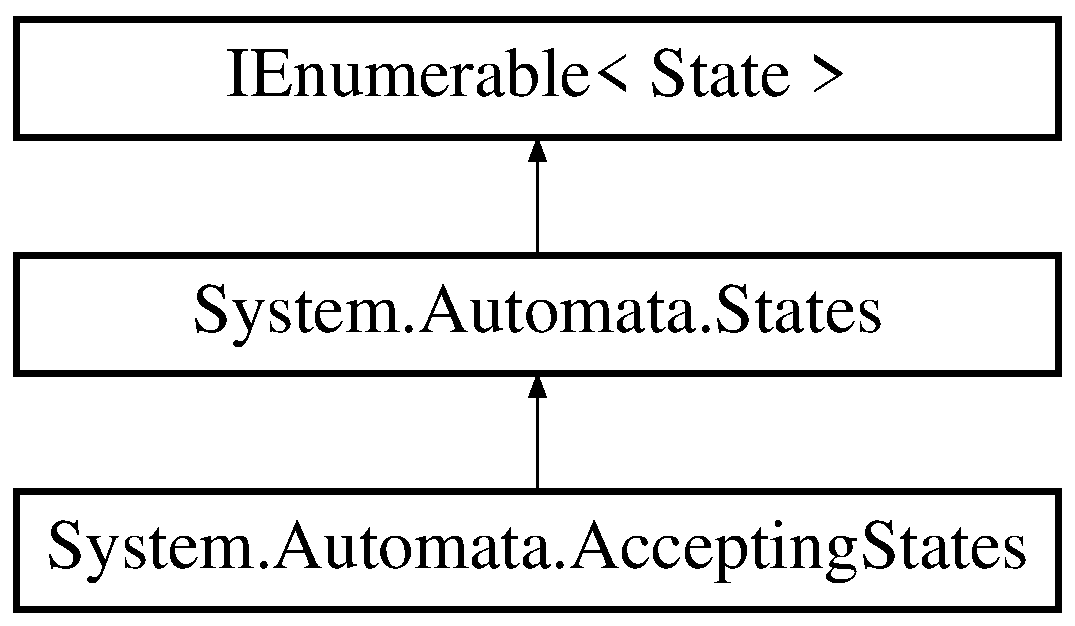
\includegraphics[height=3.000000cm]{class_system_1_1_automata_1_1_accepting_states}
\end{center}
\end{figure}
\subsection*{Public Member Functions}
\begin{DoxyCompactItemize}
\item 
\mbox{\Hypertarget{class_system_1_1_automata_1_1_accepting_states_a1a1e9e2be597a9c235c8940867466f64}\label{class_system_1_1_automata_1_1_accepting_states_a1a1e9e2be597a9c235c8940867466f64}} 
\mbox{\hyperlink{class_system_1_1_automata_1_1_accepting_states_a1a1e9e2be597a9c235c8940867466f64}{Accepting\+States}} (params \mbox{\hyperlink{class_system_1_1_automata_1_1_state}{State}}\mbox{[}$\,$\mbox{]} q)
\end{DoxyCompactItemize}
\subsection*{Additional Inherited Members}


\subsection{Detailed Description}
The set of all accepting states. 

These states should also be in the set of all states.

The documentation for this class was generated from the following file\+:\begin{DoxyCompactItemize}
\item 
System.\+Automata/Accepting\+States.\+cs\end{DoxyCompactItemize}

\hypertarget{class_system_1_1_automata_1_1_alphabet}{}\section{System.\+Automata.\+Alphabet Class Reference}
\label{class_system_1_1_automata_1_1_alphabet}\index{System.\+Automata.\+Alphabet@{System.\+Automata.\+Alphabet}}


A automaton alphabet  


Inheritance diagram for System.\+Automata.\+Alphabet\+:\begin{figure}[H]
\begin{center}
\leavevmode
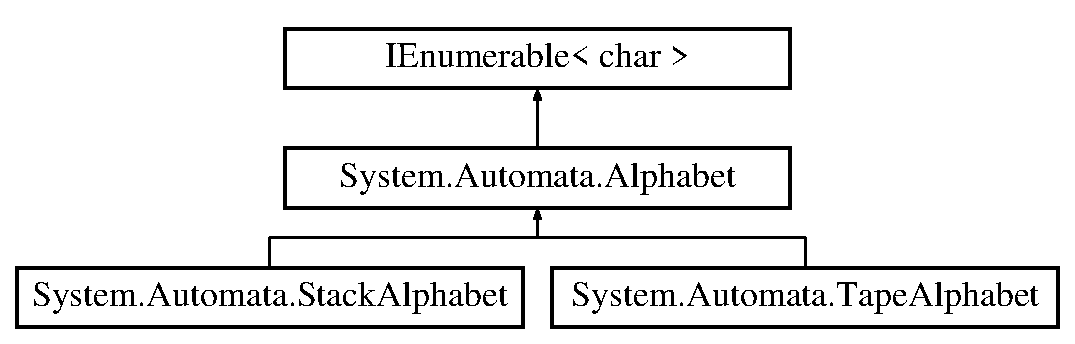
\includegraphics[height=3.000000cm]{class_system_1_1_automata_1_1_alphabet}
\end{center}
\end{figure}
\subsection*{Public Member Functions}
\begin{DoxyCompactItemize}
\item 
\mbox{\hyperlink{class_system_1_1_automata_1_1_alphabet_a890f76aaecd05e71d6ad4518cdb1cbad}{Alphabet}} (params char\mbox{[}$\,$\mbox{]} s)
\begin{DoxyCompactList}\small\item\em Initialize the alphabet with the given symbols. \end{DoxyCompactList}\item 
\mbox{\Hypertarget{class_system_1_1_automata_1_1_alphabet_a47207ac846122554bf2edd534027a4b6}\label{class_system_1_1_automata_1_1_alphabet_a47207ac846122554bf2edd534027a4b6}} 
void {\bfseries Add} (char s)
\item 
\mbox{\Hypertarget{class_system_1_1_automata_1_1_alphabet_a2470bf21c905aa98e1596a9365703d61}\label{class_system_1_1_automata_1_1_alphabet_a2470bf21c905aa98e1596a9365703d61}} 
bool {\bfseries Contains} (char s)
\item 
\mbox{\Hypertarget{class_system_1_1_automata_1_1_alphabet_a03071782ad55452e7981cd00ae2d04e8}\label{class_system_1_1_automata_1_1_alphabet_a03071782ad55452e7981cd00ae2d04e8}} 
I\+Enumerator$<$ char $>$ {\bfseries Get\+Enumerator} ()
\item 
\mbox{\Hypertarget{class_system_1_1_automata_1_1_alphabet_ae17c19674243e1b67cc77590c68ae79e}\label{class_system_1_1_automata_1_1_alphabet_ae17c19674243e1b67cc77590c68ae79e}} 
override string {\bfseries To\+String} ()
\end{DoxyCompactItemize}
\subsection*{Static Public Member Functions}
\begin{DoxyCompactItemize}
\item 
\mbox{\Hypertarget{class_system_1_1_automata_1_1_alphabet_a834a05d940b1f44a2d1d83463a16722a}\label{class_system_1_1_automata_1_1_alphabet_a834a05d940b1f44a2d1d83463a16722a}} 
static \mbox{\hyperlink{class_system_1_1_automata_1_1_alphabet}{Alphabet}} {\bfseries operator+} (\mbox{\hyperlink{class_system_1_1_automata_1_1_alphabet}{Alphabet}} a, \mbox{\hyperlink{class_system_1_1_automata_1_1_alphabet}{Alphabet}} b)
\item 
\mbox{\Hypertarget{class_system_1_1_automata_1_1_alphabet_a8cb990121ba3d7888ce8ba20782ef8d0}\label{class_system_1_1_automata_1_1_alphabet_a8cb990121ba3d7888ce8ba20782ef8d0}} 
static \mbox{\hyperlink{class_system_1_1_automata_1_1_alphabet}{Alphabet}} {\bfseries operator-\/} (\mbox{\hyperlink{class_system_1_1_automata_1_1_alphabet}{Alphabet}} a, \mbox{\hyperlink{class_system_1_1_automata_1_1_alphabet}{Alphabet}} b)
\end{DoxyCompactItemize}
\subsection*{Public Attributes}
\begin{DoxyCompactItemize}
\item 
const char \mbox{\hyperlink{class_system_1_1_automata_1_1_alphabet_aa3f8c16de4596ed24f2fe0fb77e7493c}{Empty\+String}} = \textquotesingle{}\textbackslash{}0\textquotesingle{}
\begin{DoxyCompactList}\small\item\em Represents a string of length 0 \end{DoxyCompactList}\item 
const char \mbox{\hyperlink{class_system_1_1_automata_1_1_alphabet_a1c103a38506cc7b398a6974baa5ead67}{Z}} = (char)3
\begin{DoxyCompactList}\small\item\em Represents the initial symbol on the stack. \end{DoxyCompactList}\item 
const char \mbox{\hyperlink{class_system_1_1_automata_1_1_alphabet_a16131b03673f7d6389ca4ac943881848}{Blank}} = (char)127
\begin{DoxyCompactList}\small\item\em Represents a blank symbol on a Turing tape. \end{DoxyCompactList}\item 
const char \mbox{\hyperlink{class_system_1_1_automata_1_1_alphabet_a8aa33ab3472191b4ff0234791718af25}{Wildcard}} = (char)26
\begin{DoxyCompactList}\small\item\em Represents a wildcard (?) symbol when replacing stack contents. \end{DoxyCompactList}\item 
\mbox{\Hypertarget{class_system_1_1_automata_1_1_alphabet_aec0745b87eb975303a875b829e8cc412}\label{class_system_1_1_automata_1_1_alphabet_aec0745b87eb975303a875b829e8cc412}} 
int {\bfseries Count} =$>$ Chars.\+Count
\end{DoxyCompactItemize}
\subsection*{Static Public Attributes}
\begin{DoxyCompactItemize}
\item 
static \mbox{\hyperlink{class_system_1_1_automata_1_1_alphabet}{Alphabet}} \mbox{\hyperlink{class_system_1_1_automata_1_1_alphabet_afa68a933ddc9aaa35cbeb8aa42ece58c}{Unary}} =$>$ new \mbox{\hyperlink{class_system_1_1_automata_1_1_alphabet}{Alphabet}}(\textquotesingle{}1\textquotesingle{})
\begin{DoxyCompactList}\small\item\em \{1\} \end{DoxyCompactList}\item 
static \mbox{\hyperlink{class_system_1_1_automata_1_1_alphabet}{Alphabet}} \mbox{\hyperlink{class_system_1_1_automata_1_1_alphabet_a33781b08f0b9a39f1da39ee85fd69fb3}{Binary}} =$>$ new \mbox{\hyperlink{class_system_1_1_automata_1_1_alphabet}{Alphabet}}(\textquotesingle{}0\textquotesingle{}, \textquotesingle{}1\textquotesingle{})
\begin{DoxyCompactList}\small\item\em \{0, 1\} \end{DoxyCompactList}\item 
static \mbox{\hyperlink{class_system_1_1_automata_1_1_alphabet}{Alphabet}} \mbox{\hyperlink{class_system_1_1_automata_1_1_alphabet_a815270890b0afe881cfa7af15b4a4895}{Decimal}} =$>$ new \mbox{\hyperlink{class_system_1_1_automata_1_1_alphabet}{Alphabet}}(Enumerable.\+Range(48, 10).Select(c =$>$ (char)c).To\+Array())
\begin{DoxyCompactList}\small\item\em \{0, 1, ..., 9\} \end{DoxyCompactList}\item 
static \mbox{\hyperlink{class_system_1_1_automata_1_1_alphabet}{Alphabet}} \mbox{\hyperlink{class_system_1_1_automata_1_1_alphabet_a5040c44fbca9ecf1348714c74b848b1d}{Ab}} =$>$ new \mbox{\hyperlink{class_system_1_1_automata_1_1_alphabet}{Alphabet}}(\textquotesingle{}a\textquotesingle{}, \textquotesingle{}b\textquotesingle{})
\begin{DoxyCompactList}\small\item\em \{a, b\} \end{DoxyCompactList}\item 
static \mbox{\hyperlink{class_system_1_1_automata_1_1_alphabet}{Alphabet}} \mbox{\hyperlink{class_system_1_1_automata_1_1_alphabet_a2c79b315618446cdd7ba875a7924d83f}{Abc}} =$>$ new \mbox{\hyperlink{class_system_1_1_automata_1_1_alphabet}{Alphabet}}(\textquotesingle{}a\textquotesingle{}, \textquotesingle{}b\textquotesingle{}, \textquotesingle{}c\textquotesingle{})
\begin{DoxyCompactList}\small\item\em \{a, b, c\} \end{DoxyCompactList}\item 
static \mbox{\hyperlink{class_system_1_1_automata_1_1_alphabet}{Alphabet}} \mbox{\hyperlink{class_system_1_1_automata_1_1_alphabet_a6962b8539b792f5b1c00401f45894b58}{Az\+Lower}} =$>$ new \mbox{\hyperlink{class_system_1_1_automata_1_1_alphabet}{Alphabet}}(Enumerable.\+Range(65, 26).Select(c =$>$ (char)c).To\+Array())
\begin{DoxyCompactList}\small\item\em \{a, b, ..., z\} \end{DoxyCompactList}\item 
static \mbox{\hyperlink{class_system_1_1_automata_1_1_alphabet}{Alphabet}} \mbox{\hyperlink{class_system_1_1_automata_1_1_alphabet_ac1b4eaec3c00e63dab2d176773ec84f1}{Az\+Upper}} =$>$ new \mbox{\hyperlink{class_system_1_1_automata_1_1_alphabet}{Alphabet}}(Enumerable.\+Range(97, 26).Select(c =$>$ (char)c).To\+Array())
\begin{DoxyCompactList}\small\item\em \{A, B, ..., Z\} \end{DoxyCompactList}\item 
static \mbox{\hyperlink{class_system_1_1_automata_1_1_alphabet}{Alphabet}} \mbox{\hyperlink{class_system_1_1_automata_1_1_alphabet_a090b19b9683fc56693e032edf961313f}{Az\+All}} =$>$ new \mbox{\hyperlink{class_system_1_1_automata_1_1_alphabet}{Alphabet}}(Az\+Lower.\+Concat(\mbox{\hyperlink{class_system_1_1_automata_1_1_alphabet_ac1b4eaec3c00e63dab2d176773ec84f1}{Az\+Upper}}).To\+Array())
\begin{DoxyCompactList}\small\item\em \{a, b, ..., Z\} \end{DoxyCompactList}\item 
static \mbox{\hyperlink{class_system_1_1_automata_1_1_alphabet}{Alphabet}} \mbox{\hyperlink{class_system_1_1_automata_1_1_alphabet_a8876c9767b18e483848a0f4bc4de2cef}{Ascii}} =$>$ new \mbox{\hyperlink{class_system_1_1_automata_1_1_alphabet}{Alphabet}}(Enumerable.\+Range(32, 94).Select(c =$>$ (char)c).To\+Array())
\begin{DoxyCompactList}\small\item\em All the printable A\+S\+C\+II characters \end{DoxyCompactList}\end{DoxyCompactItemize}
\subsection*{Protected Attributes}
\begin{DoxyCompactItemize}
\item 
\mbox{\Hypertarget{class_system_1_1_automata_1_1_alphabet_af772a1899e075c880b75bdc12e4fc766}\label{class_system_1_1_automata_1_1_alphabet_af772a1899e075c880b75bdc12e4fc766}} 
List$<$ char $>$ {\bfseries Chars}
\end{DoxyCompactItemize}


\subsection{Detailed Description}
A automaton alphabet 



\subsection{Constructor \& Destructor Documentation}
\mbox{\Hypertarget{class_system_1_1_automata_1_1_alphabet_a890f76aaecd05e71d6ad4518cdb1cbad}\label{class_system_1_1_automata_1_1_alphabet_a890f76aaecd05e71d6ad4518cdb1cbad}} 
\index{System\+::\+Automata\+::\+Alphabet@{System\+::\+Automata\+::\+Alphabet}!Alphabet@{Alphabet}}
\index{Alphabet@{Alphabet}!System\+::\+Automata\+::\+Alphabet@{System\+::\+Automata\+::\+Alphabet}}
\subsubsection{\texorpdfstring{Alphabet()}{Alphabet()}}
{\footnotesize\ttfamily System.\+Automata.\+Alphabet.\+Alphabet (\begin{DoxyParamCaption}\item[{params char \mbox{[}$\,$\mbox{]}}]{s }\end{DoxyParamCaption})}



Initialize the alphabet with the given symbols. 


\begin{DoxyParams}{Parameters}
{\em s} & The symbols to use.\\
\hline
\end{DoxyParams}


\subsection{Member Data Documentation}
\mbox{\Hypertarget{class_system_1_1_automata_1_1_alphabet_a5040c44fbca9ecf1348714c74b848b1d}\label{class_system_1_1_automata_1_1_alphabet_a5040c44fbca9ecf1348714c74b848b1d}} 
\index{System\+::\+Automata\+::\+Alphabet@{System\+::\+Automata\+::\+Alphabet}!Ab@{Ab}}
\index{Ab@{Ab}!System\+::\+Automata\+::\+Alphabet@{System\+::\+Automata\+::\+Alphabet}}
\subsubsection{\texorpdfstring{Ab}{Ab}}
{\footnotesize\ttfamily \mbox{\hyperlink{class_system_1_1_automata_1_1_alphabet}{Alphabet}} System.\+Automata.\+Alphabet.\+Ab =$>$ new \mbox{\hyperlink{class_system_1_1_automata_1_1_alphabet}{Alphabet}}(\textquotesingle{}a\textquotesingle{}, \textquotesingle{}b\textquotesingle{})\hspace{0.3cm}{\ttfamily [static]}}



\{a, b\} 

\mbox{\Hypertarget{class_system_1_1_automata_1_1_alphabet_a2c79b315618446cdd7ba875a7924d83f}\label{class_system_1_1_automata_1_1_alphabet_a2c79b315618446cdd7ba875a7924d83f}} 
\index{System\+::\+Automata\+::\+Alphabet@{System\+::\+Automata\+::\+Alphabet}!Abc@{Abc}}
\index{Abc@{Abc}!System\+::\+Automata\+::\+Alphabet@{System\+::\+Automata\+::\+Alphabet}}
\subsubsection{\texorpdfstring{Abc}{Abc}}
{\footnotesize\ttfamily \mbox{\hyperlink{class_system_1_1_automata_1_1_alphabet}{Alphabet}} System.\+Automata.\+Alphabet.\+Abc =$>$ new \mbox{\hyperlink{class_system_1_1_automata_1_1_alphabet}{Alphabet}}(\textquotesingle{}a\textquotesingle{}, \textquotesingle{}b\textquotesingle{}, \textquotesingle{}c\textquotesingle{})\hspace{0.3cm}{\ttfamily [static]}}



\{a, b, c\} 

\mbox{\Hypertarget{class_system_1_1_automata_1_1_alphabet_a8876c9767b18e483848a0f4bc4de2cef}\label{class_system_1_1_automata_1_1_alphabet_a8876c9767b18e483848a0f4bc4de2cef}} 
\index{System\+::\+Automata\+::\+Alphabet@{System\+::\+Automata\+::\+Alphabet}!Ascii@{Ascii}}
\index{Ascii@{Ascii}!System\+::\+Automata\+::\+Alphabet@{System\+::\+Automata\+::\+Alphabet}}
\subsubsection{\texorpdfstring{Ascii}{Ascii}}
{\footnotesize\ttfamily \mbox{\hyperlink{class_system_1_1_automata_1_1_alphabet}{Alphabet}} System.\+Automata.\+Alphabet.\+Ascii =$>$ new \mbox{\hyperlink{class_system_1_1_automata_1_1_alphabet}{Alphabet}}(Enumerable.\+Range(32, 94).Select(c =$>$ (char)c).To\+Array())\hspace{0.3cm}{\ttfamily [static]}}



All the printable A\+S\+C\+II characters 

\mbox{\Hypertarget{class_system_1_1_automata_1_1_alphabet_a090b19b9683fc56693e032edf961313f}\label{class_system_1_1_automata_1_1_alphabet_a090b19b9683fc56693e032edf961313f}} 
\index{System\+::\+Automata\+::\+Alphabet@{System\+::\+Automata\+::\+Alphabet}!Az\+All@{Az\+All}}
\index{Az\+All@{Az\+All}!System\+::\+Automata\+::\+Alphabet@{System\+::\+Automata\+::\+Alphabet}}
\subsubsection{\texorpdfstring{Az\+All}{AzAll}}
{\footnotesize\ttfamily \mbox{\hyperlink{class_system_1_1_automata_1_1_alphabet}{Alphabet}} System.\+Automata.\+Alphabet.\+Az\+All =$>$ new \mbox{\hyperlink{class_system_1_1_automata_1_1_alphabet}{Alphabet}}(Az\+Lower.\+Concat(\mbox{\hyperlink{class_system_1_1_automata_1_1_alphabet_ac1b4eaec3c00e63dab2d176773ec84f1}{Az\+Upper}}).To\+Array())\hspace{0.3cm}{\ttfamily [static]}}



\{a, b, ..., Z\} 

\mbox{\Hypertarget{class_system_1_1_automata_1_1_alphabet_a6962b8539b792f5b1c00401f45894b58}\label{class_system_1_1_automata_1_1_alphabet_a6962b8539b792f5b1c00401f45894b58}} 
\index{System\+::\+Automata\+::\+Alphabet@{System\+::\+Automata\+::\+Alphabet}!Az\+Lower@{Az\+Lower}}
\index{Az\+Lower@{Az\+Lower}!System\+::\+Automata\+::\+Alphabet@{System\+::\+Automata\+::\+Alphabet}}
\subsubsection{\texorpdfstring{Az\+Lower}{AzLower}}
{\footnotesize\ttfamily \mbox{\hyperlink{class_system_1_1_automata_1_1_alphabet}{Alphabet}} System.\+Automata.\+Alphabet.\+Az\+Lower =$>$ new \mbox{\hyperlink{class_system_1_1_automata_1_1_alphabet}{Alphabet}}(Enumerable.\+Range(65, 26).Select(c =$>$ (char)c).To\+Array())\hspace{0.3cm}{\ttfamily [static]}}



\{a, b, ..., z\} 

\mbox{\Hypertarget{class_system_1_1_automata_1_1_alphabet_ac1b4eaec3c00e63dab2d176773ec84f1}\label{class_system_1_1_automata_1_1_alphabet_ac1b4eaec3c00e63dab2d176773ec84f1}} 
\index{System\+::\+Automata\+::\+Alphabet@{System\+::\+Automata\+::\+Alphabet}!Az\+Upper@{Az\+Upper}}
\index{Az\+Upper@{Az\+Upper}!System\+::\+Automata\+::\+Alphabet@{System\+::\+Automata\+::\+Alphabet}}
\subsubsection{\texorpdfstring{Az\+Upper}{AzUpper}}
{\footnotesize\ttfamily \mbox{\hyperlink{class_system_1_1_automata_1_1_alphabet}{Alphabet}} System.\+Automata.\+Alphabet.\+Az\+Upper =$>$ new \mbox{\hyperlink{class_system_1_1_automata_1_1_alphabet}{Alphabet}}(Enumerable.\+Range(97, 26).Select(c =$>$ (char)c).To\+Array())\hspace{0.3cm}{\ttfamily [static]}}



\{A, B, ..., Z\} 

\mbox{\Hypertarget{class_system_1_1_automata_1_1_alphabet_a33781b08f0b9a39f1da39ee85fd69fb3}\label{class_system_1_1_automata_1_1_alphabet_a33781b08f0b9a39f1da39ee85fd69fb3}} 
\index{System\+::\+Automata\+::\+Alphabet@{System\+::\+Automata\+::\+Alphabet}!Binary@{Binary}}
\index{Binary@{Binary}!System\+::\+Automata\+::\+Alphabet@{System\+::\+Automata\+::\+Alphabet}}
\subsubsection{\texorpdfstring{Binary}{Binary}}
{\footnotesize\ttfamily \mbox{\hyperlink{class_system_1_1_automata_1_1_alphabet}{Alphabet}} System.\+Automata.\+Alphabet.\+Binary =$>$ new \mbox{\hyperlink{class_system_1_1_automata_1_1_alphabet}{Alphabet}}(\textquotesingle{}0\textquotesingle{}, \textquotesingle{}1\textquotesingle{})\hspace{0.3cm}{\ttfamily [static]}}



\{0, 1\} 

\mbox{\Hypertarget{class_system_1_1_automata_1_1_alphabet_a16131b03673f7d6389ca4ac943881848}\label{class_system_1_1_automata_1_1_alphabet_a16131b03673f7d6389ca4ac943881848}} 
\index{System\+::\+Automata\+::\+Alphabet@{System\+::\+Automata\+::\+Alphabet}!Blank@{Blank}}
\index{Blank@{Blank}!System\+::\+Automata\+::\+Alphabet@{System\+::\+Automata\+::\+Alphabet}}
\subsubsection{\texorpdfstring{Blank}{Blank}}
{\footnotesize\ttfamily const char System.\+Automata.\+Alphabet.\+Blank = (char)127}



Represents a blank symbol on a Turing tape. 

\mbox{\Hypertarget{class_system_1_1_automata_1_1_alphabet_a815270890b0afe881cfa7af15b4a4895}\label{class_system_1_1_automata_1_1_alphabet_a815270890b0afe881cfa7af15b4a4895}} 
\index{System\+::\+Automata\+::\+Alphabet@{System\+::\+Automata\+::\+Alphabet}!Decimal@{Decimal}}
\index{Decimal@{Decimal}!System\+::\+Automata\+::\+Alphabet@{System\+::\+Automata\+::\+Alphabet}}
\subsubsection{\texorpdfstring{Decimal}{Decimal}}
{\footnotesize\ttfamily \mbox{\hyperlink{class_system_1_1_automata_1_1_alphabet}{Alphabet}} System.\+Automata.\+Alphabet.\+Decimal =$>$ new \mbox{\hyperlink{class_system_1_1_automata_1_1_alphabet}{Alphabet}}(Enumerable.\+Range(48, 10).Select(c =$>$ (char)c).To\+Array())\hspace{0.3cm}{\ttfamily [static]}}



\{0, 1, ..., 9\} 

\mbox{\Hypertarget{class_system_1_1_automata_1_1_alphabet_aa3f8c16de4596ed24f2fe0fb77e7493c}\label{class_system_1_1_automata_1_1_alphabet_aa3f8c16de4596ed24f2fe0fb77e7493c}} 
\index{System\+::\+Automata\+::\+Alphabet@{System\+::\+Automata\+::\+Alphabet}!Empty\+String@{Empty\+String}}
\index{Empty\+String@{Empty\+String}!System\+::\+Automata\+::\+Alphabet@{System\+::\+Automata\+::\+Alphabet}}
\subsubsection{\texorpdfstring{Empty\+String}{EmptyString}}
{\footnotesize\ttfamily const char System.\+Automata.\+Alphabet.\+Empty\+String = \textquotesingle{}\textbackslash{}0\textquotesingle{}}



Represents a string of length 0 

\mbox{\Hypertarget{class_system_1_1_automata_1_1_alphabet_afa68a933ddc9aaa35cbeb8aa42ece58c}\label{class_system_1_1_automata_1_1_alphabet_afa68a933ddc9aaa35cbeb8aa42ece58c}} 
\index{System\+::\+Automata\+::\+Alphabet@{System\+::\+Automata\+::\+Alphabet}!Unary@{Unary}}
\index{Unary@{Unary}!System\+::\+Automata\+::\+Alphabet@{System\+::\+Automata\+::\+Alphabet}}
\subsubsection{\texorpdfstring{Unary}{Unary}}
{\footnotesize\ttfamily \mbox{\hyperlink{class_system_1_1_automata_1_1_alphabet}{Alphabet}} System.\+Automata.\+Alphabet.\+Unary =$>$ new \mbox{\hyperlink{class_system_1_1_automata_1_1_alphabet}{Alphabet}}(\textquotesingle{}1\textquotesingle{})\hspace{0.3cm}{\ttfamily [static]}}



\{1\} 

\mbox{\Hypertarget{class_system_1_1_automata_1_1_alphabet_a8aa33ab3472191b4ff0234791718af25}\label{class_system_1_1_automata_1_1_alphabet_a8aa33ab3472191b4ff0234791718af25}} 
\index{System\+::\+Automata\+::\+Alphabet@{System\+::\+Automata\+::\+Alphabet}!Wildcard@{Wildcard}}
\index{Wildcard@{Wildcard}!System\+::\+Automata\+::\+Alphabet@{System\+::\+Automata\+::\+Alphabet}}
\subsubsection{\texorpdfstring{Wildcard}{Wildcard}}
{\footnotesize\ttfamily const char System.\+Automata.\+Alphabet.\+Wildcard = (char)26}



Represents a wildcard (?) symbol when replacing stack contents. 

\mbox{\Hypertarget{class_system_1_1_automata_1_1_alphabet_a1c103a38506cc7b398a6974baa5ead67}\label{class_system_1_1_automata_1_1_alphabet_a1c103a38506cc7b398a6974baa5ead67}} 
\index{System\+::\+Automata\+::\+Alphabet@{System\+::\+Automata\+::\+Alphabet}!Z@{Z}}
\index{Z@{Z}!System\+::\+Automata\+::\+Alphabet@{System\+::\+Automata\+::\+Alphabet}}
\subsubsection{\texorpdfstring{Z}{Z}}
{\footnotesize\ttfamily const char System.\+Automata.\+Alphabet.\+Z = (char)3}



Represents the initial symbol on the stack. 



The documentation for this class was generated from the following file\+:\begin{DoxyCompactItemize}
\item 
System.\+Automata/Alphabet.\+cs\end{DoxyCompactItemize}

\hypertarget{class_system_1_1_automata_1_1_automaton}{}\section{System.\+Automata.\+Automaton Class Reference}
\label{class_system_1_1_automata_1_1_automaton}\index{System.\+Automata.\+Automaton@{System.\+Automata.\+Automaton}}
Inheritance diagram for System.\+Automata.\+Automaton\+:\begin{figure}[H]
\begin{center}
\leavevmode
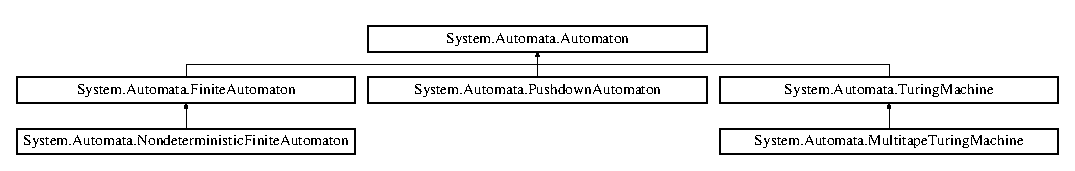
\includegraphics[height=1.848185cm]{class_system_1_1_automata_1_1_automaton}
\end{center}
\end{figure}
\subsection*{Properties}
\begin{DoxyCompactItemize}
\item 
\mbox{\hyperlink{class_system_1_1_automata_1_1_states}{States}} \mbox{\hyperlink{class_system_1_1_automata_1_1_automaton_a21fc2f1e7cf4ee121de2547dc184dedf}{States}}\hspace{0.3cm}{\ttfamily  \mbox{[}get, protected set\mbox{]}}
\begin{DoxyCompactList}\small\item\em The set of states. \end{DoxyCompactList}\item 
\mbox{\hyperlink{class_system_1_1_automata_1_1_accepting_states}{Accepting\+States}} \mbox{\hyperlink{class_system_1_1_automata_1_1_automaton_a393c78f68acc96e815f02a2f8ca34011}{Accepting\+States}}\hspace{0.3cm}{\ttfamily  \mbox{[}get, protected set\mbox{]}}
\begin{DoxyCompactList}\small\item\em The set of accepting states. \end{DoxyCompactList}\item 
\mbox{\hyperlink{class_system_1_1_automata_1_1_alphabet}{Alphabet}} \mbox{\hyperlink{class_system_1_1_automata_1_1_automaton_ac18c40e73b9b787f2d3084e65110929d}{Alphabet}}\hspace{0.3cm}{\ttfamily  \mbox{[}get, protected set\mbox{]}}
\begin{DoxyCompactList}\small\item\em The machine\textquotesingle{}s alphabet. \end{DoxyCompactList}\item 
\mbox{\hyperlink{class_system_1_1_automata_1_1_state}{State}} \mbox{\hyperlink{class_system_1_1_automata_1_1_automaton_a827b16190eb21a97ee14ff46274b0029}{Initial\+State}}\hspace{0.3cm}{\ttfamily  \mbox{[}get, protected set\mbox{]}}
\begin{DoxyCompactList}\small\item\em The initial state. \end{DoxyCompactList}\item 
\mbox{\hyperlink{class_system_1_1_automata_1_1_transition_function}{Transition\+Function}} \mbox{\hyperlink{class_system_1_1_automata_1_1_automaton_ae109aca0f6f80efc50e9553cfe250ce5}{Transitions}}\hspace{0.3cm}{\ttfamily  \mbox{[}get, protected set\mbox{]}}
\begin{DoxyCompactList}\small\item\em The state transition mappings \end{DoxyCompactList}\end{DoxyCompactItemize}


\subsection{Property Documentation}
\mbox{\Hypertarget{class_system_1_1_automata_1_1_automaton_a393c78f68acc96e815f02a2f8ca34011}\label{class_system_1_1_automata_1_1_automaton_a393c78f68acc96e815f02a2f8ca34011}} 
\index{System\+::\+Automata\+::\+Automaton@{System\+::\+Automata\+::\+Automaton}!Accepting\+States@{Accepting\+States}}
\index{Accepting\+States@{Accepting\+States}!System\+::\+Automata\+::\+Automaton@{System\+::\+Automata\+::\+Automaton}}
\subsubsection{\texorpdfstring{Accepting\+States}{AcceptingStates}}
{\footnotesize\ttfamily \mbox{\hyperlink{class_system_1_1_automata_1_1_accepting_states}{Accepting\+States}} System.\+Automata.\+Automaton.\+Accepting\+States\hspace{0.3cm}{\ttfamily [get]}, {\ttfamily [protected set]}}



The set of accepting states. 

\mbox{\Hypertarget{class_system_1_1_automata_1_1_automaton_ac18c40e73b9b787f2d3084e65110929d}\label{class_system_1_1_automata_1_1_automaton_ac18c40e73b9b787f2d3084e65110929d}} 
\index{System\+::\+Automata\+::\+Automaton@{System\+::\+Automata\+::\+Automaton}!Alphabet@{Alphabet}}
\index{Alphabet@{Alphabet}!System\+::\+Automata\+::\+Automaton@{System\+::\+Automata\+::\+Automaton}}
\subsubsection{\texorpdfstring{Alphabet}{Alphabet}}
{\footnotesize\ttfamily \mbox{\hyperlink{class_system_1_1_automata_1_1_alphabet}{Alphabet}} System.\+Automata.\+Automaton.\+Alphabet\hspace{0.3cm}{\ttfamily [get]}, {\ttfamily [protected set]}}



The machine\textquotesingle{}s alphabet. 

\mbox{\Hypertarget{class_system_1_1_automata_1_1_automaton_a827b16190eb21a97ee14ff46274b0029}\label{class_system_1_1_automata_1_1_automaton_a827b16190eb21a97ee14ff46274b0029}} 
\index{System\+::\+Automata\+::\+Automaton@{System\+::\+Automata\+::\+Automaton}!Initial\+State@{Initial\+State}}
\index{Initial\+State@{Initial\+State}!System\+::\+Automata\+::\+Automaton@{System\+::\+Automata\+::\+Automaton}}
\subsubsection{\texorpdfstring{Initial\+State}{InitialState}}
{\footnotesize\ttfamily \mbox{\hyperlink{class_system_1_1_automata_1_1_state}{State}} System.\+Automata.\+Automaton.\+Initial\+State\hspace{0.3cm}{\ttfamily [get]}, {\ttfamily [protected set]}}



The initial state. 

\mbox{\Hypertarget{class_system_1_1_automata_1_1_automaton_a21fc2f1e7cf4ee121de2547dc184dedf}\label{class_system_1_1_automata_1_1_automaton_a21fc2f1e7cf4ee121de2547dc184dedf}} 
\index{System\+::\+Automata\+::\+Automaton@{System\+::\+Automata\+::\+Automaton}!States@{States}}
\index{States@{States}!System\+::\+Automata\+::\+Automaton@{System\+::\+Automata\+::\+Automaton}}
\subsubsection{\texorpdfstring{States}{States}}
{\footnotesize\ttfamily \mbox{\hyperlink{class_system_1_1_automata_1_1_states}{States}} System.\+Automata.\+Automaton.\+States\hspace{0.3cm}{\ttfamily [get]}, {\ttfamily [protected set]}}



The set of states. 

\mbox{\Hypertarget{class_system_1_1_automata_1_1_automaton_ae109aca0f6f80efc50e9553cfe250ce5}\label{class_system_1_1_automata_1_1_automaton_ae109aca0f6f80efc50e9553cfe250ce5}} 
\index{System\+::\+Automata\+::\+Automaton@{System\+::\+Automata\+::\+Automaton}!Transitions@{Transitions}}
\index{Transitions@{Transitions}!System\+::\+Automata\+::\+Automaton@{System\+::\+Automata\+::\+Automaton}}
\subsubsection{\texorpdfstring{Transitions}{Transitions}}
{\footnotesize\ttfamily \mbox{\hyperlink{class_system_1_1_automata_1_1_transition_function}{Transition\+Function}} System.\+Automata.\+Automaton.\+Transitions\hspace{0.3cm}{\ttfamily [get]}, {\ttfamily [protected set]}}



The state transition mappings 



The documentation for this class was generated from the following file\+:\begin{DoxyCompactItemize}
\item 
System.\+Automata/Automaton.\+cs\end{DoxyCompactItemize}

\hypertarget{class_system_1_1_automata_1_1_finite_automaton}{}\section{System.\+Automata.\+Finite\+Automaton Class Reference}
\label{class_system_1_1_automata_1_1_finite_automaton}\index{System.\+Automata.\+Finite\+Automaton@{System.\+Automata.\+Finite\+Automaton}}


A deterministic Finite \mbox{\hyperlink{class_system_1_1_automata_1_1_automaton}{Automaton}}  


Inheritance diagram for System.\+Automata.\+Finite\+Automaton\+:\begin{figure}[H]
\begin{center}
\leavevmode
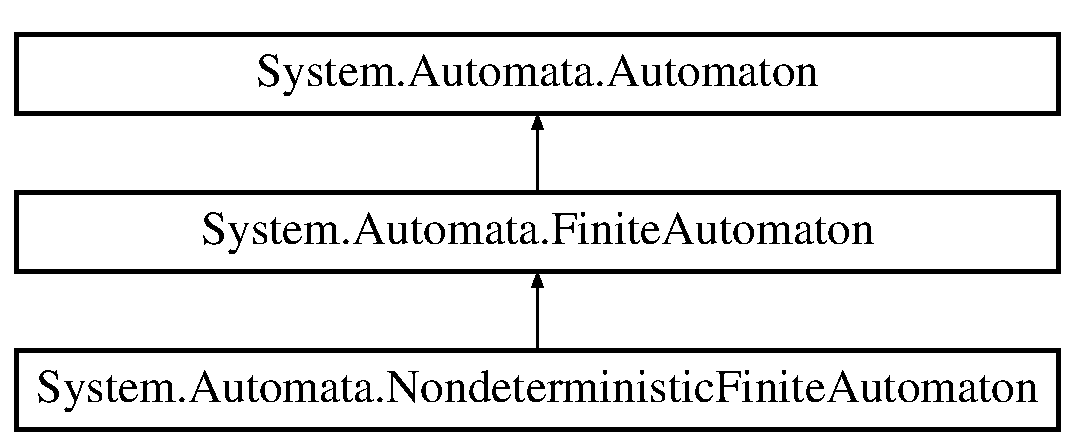
\includegraphics[height=3.000000cm]{class_system_1_1_automata_1_1_finite_automaton}
\end{center}
\end{figure}
\subsection*{Public Member Functions}
\begin{DoxyCompactItemize}
\item 
\mbox{\Hypertarget{class_system_1_1_automata_1_1_finite_automaton_a6ac4737d865c3df8657ed1814b47905d}\label{class_system_1_1_automata_1_1_finite_automaton_a6ac4737d865c3df8657ed1814b47905d}} 
{\bfseries Finite\+Automaton} (\mbox{\hyperlink{class_system_1_1_automata_1_1_states}{States}} q, \mbox{\hyperlink{class_system_1_1_automata_1_1_alphabet}{Alphabet}} a, \mbox{\hyperlink{class_system_1_1_automata_1_1_transition_function}{Transition\+Function}} d, \mbox{\hyperlink{class_system_1_1_automata_1_1_state}{State}} q0, \mbox{\hyperlink{class_system_1_1_automata_1_1_accepting_states}{Accepting\+States}} f)
\item 
bool \mbox{\hyperlink{class_system_1_1_automata_1_1_finite_automaton_a8c6c352f912d13d5a0047583a34247db}{Run}} (char\mbox{[}$\,$\mbox{]} x)
\begin{DoxyCompactList}\small\item\em Run the machine using the given input. \end{DoxyCompactList}\item 
bool \mbox{\hyperlink{class_system_1_1_automata_1_1_finite_automaton_aaa76a2104f685809c00c7adc8ceb240f}{Run}} (string x)
\begin{DoxyCompactList}\small\item\em Run the machine using the given input. \end{DoxyCompactList}\end{DoxyCompactItemize}
\subsection*{Additional Inherited Members}


\subsection{Detailed Description}
A deterministic Finite \mbox{\hyperlink{class_system_1_1_automata_1_1_automaton}{Automaton}} 



\subsection{Member Function Documentation}
\mbox{\Hypertarget{class_system_1_1_automata_1_1_finite_automaton_a8c6c352f912d13d5a0047583a34247db}\label{class_system_1_1_automata_1_1_finite_automaton_a8c6c352f912d13d5a0047583a34247db}} 
\index{System\+::\+Automata\+::\+Finite\+Automaton@{System\+::\+Automata\+::\+Finite\+Automaton}!Run@{Run}}
\index{Run@{Run}!System\+::\+Automata\+::\+Finite\+Automaton@{System\+::\+Automata\+::\+Finite\+Automaton}}
\subsubsection{\texorpdfstring{Run()}{Run()}\hspace{0.1cm}{\footnotesize\ttfamily [1/2]}}
{\footnotesize\ttfamily bool System.\+Automata.\+Finite\+Automaton.\+Run (\begin{DoxyParamCaption}\item[{char \mbox{[}$\,$\mbox{]}}]{x }\end{DoxyParamCaption})}



Run the machine using the given input. 


\begin{DoxyParams}{Parameters}
{\em x} & The input string.\\
\hline
\end{DoxyParams}
\begin{DoxyReturn}{Returns}
True if the machine accepts the input string.
\end{DoxyReturn}
\mbox{\Hypertarget{class_system_1_1_automata_1_1_finite_automaton_aaa76a2104f685809c00c7adc8ceb240f}\label{class_system_1_1_automata_1_1_finite_automaton_aaa76a2104f685809c00c7adc8ceb240f}} 
\index{System\+::\+Automata\+::\+Finite\+Automaton@{System\+::\+Automata\+::\+Finite\+Automaton}!Run@{Run}}
\index{Run@{Run}!System\+::\+Automata\+::\+Finite\+Automaton@{System\+::\+Automata\+::\+Finite\+Automaton}}
\subsubsection{\texorpdfstring{Run()}{Run()}\hspace{0.1cm}{\footnotesize\ttfamily [2/2]}}
{\footnotesize\ttfamily bool System.\+Automata.\+Finite\+Automaton.\+Run (\begin{DoxyParamCaption}\item[{string}]{x }\end{DoxyParamCaption})}



Run the machine using the given input. 


\begin{DoxyParams}{Parameters}
{\em x} & The input string.\\
\hline
\end{DoxyParams}
\begin{DoxyReturn}{Returns}
True if the machine accepts the input string.
\end{DoxyReturn}


The documentation for this class was generated from the following file\+:\begin{DoxyCompactItemize}
\item 
System.\+Automata/Finite\+Automaton.\+cs\end{DoxyCompactItemize}

\hypertarget{class_system_1_1_automata_1_1_multitape_turing_machine}{}\section{System.\+Automata.\+Multitape\+Turing\+Machine Class Reference}
\label{class_system_1_1_automata_1_1_multitape_turing_machine}\index{System.\+Automata.\+Multitape\+Turing\+Machine@{System.\+Automata.\+Multitape\+Turing\+Machine}}
Inheritance diagram for System.\+Automata.\+Multitape\+Turing\+Machine\+:\begin{figure}[H]
\begin{center}
\leavevmode
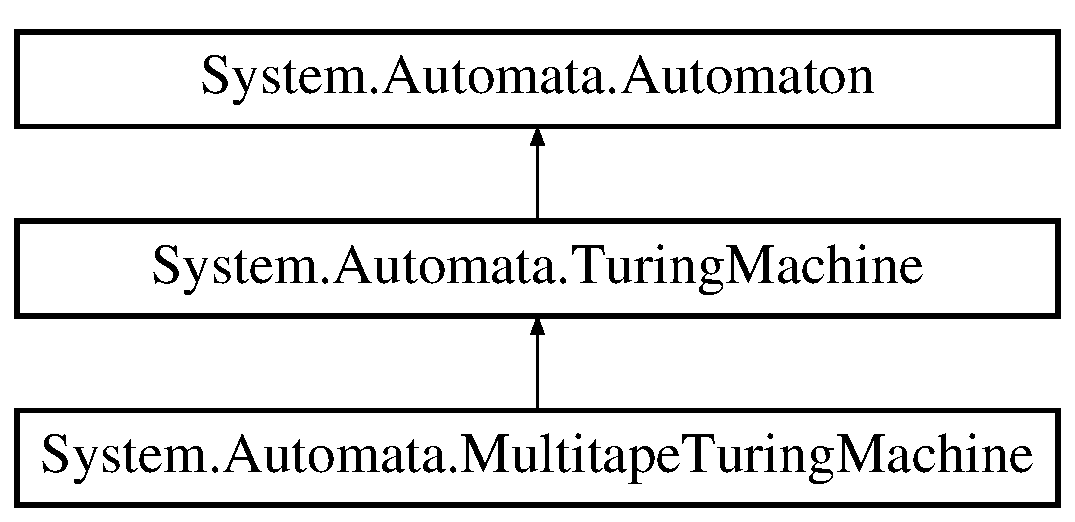
\includegraphics[height=3.000000cm]{class_system_1_1_automata_1_1_multitape_turing_machine}
\end{center}
\end{figure}
\subsection*{Public Member Functions}
\begin{DoxyCompactItemize}
\item 
\mbox{\Hypertarget{class_system_1_1_automata_1_1_multitape_turing_machine_afc461c5047fd4f27545eceae4110791f}\label{class_system_1_1_automata_1_1_multitape_turing_machine_afc461c5047fd4f27545eceae4110791f}} 
{\bfseries Multitape\+Turing\+Machine} (\mbox{\hyperlink{class_system_1_1_automata_1_1_states}{States}} q, \mbox{\hyperlink{class_system_1_1_automata_1_1_alphabet}{Alphabet}} a, \mbox{\hyperlink{class_system_1_1_automata_1_1_tape_alphabet}{Tape\+Alphabet}} g, \mbox{\hyperlink{class_system_1_1_automata_1_1_multitape_turing_transition_function}{Multitape\+Turing\+Transition\+Function}} tf, \mbox{\hyperlink{class_system_1_1_automata_1_1_state}{State}} q0, int k=1)
\item 
\mbox{\Hypertarget{class_system_1_1_automata_1_1_multitape_turing_machine_a39f81dc6eaad76473b0771a75f6cd82c}\label{class_system_1_1_automata_1_1_multitape_turing_machine_a39f81dc6eaad76473b0771a75f6cd82c}} 
new bool {\bfseries Run} (string x)
\item 
\mbox{\Hypertarget{class_system_1_1_automata_1_1_multitape_turing_machine_a426056ee2d8989e27ae31667ec6dfc40}\label{class_system_1_1_automata_1_1_multitape_turing_machine_a426056ee2d8989e27ae31667ec6dfc40}} 
new bool {\bfseries Run} (string x, out char\mbox{[}$\,$\mbox{]} o)
\item 
new bool \mbox{\hyperlink{class_system_1_1_automata_1_1_multitape_turing_machine_abc213e915db06cf43250f4739ade5779}{Run}} (I\+Enumerable$<$ char $>$ x)
\begin{DoxyCompactList}\small\item\em Run the machine \end{DoxyCompactList}\item 
\mbox{\Hypertarget{class_system_1_1_automata_1_1_multitape_turing_machine_a0d62cbc26d821e1200eecd1160eeaecd}\label{class_system_1_1_automata_1_1_multitape_turing_machine_a0d62cbc26d821e1200eecd1160eeaecd}} 
new bool {\bfseries Run} (I\+Enumerable$<$ char $>$ x, out char\mbox{[}$\,$\mbox{]} o)
\end{DoxyCompactItemize}
\subsection*{Properties}
\begin{DoxyCompactItemize}
\item 
new \mbox{\hyperlink{class_system_1_1_automata_1_1_multitape_turing_transition_function}{Multitape\+Turing\+Transition\+Function}} \mbox{\hyperlink{class_system_1_1_automata_1_1_multitape_turing_machine_a89737fb1fa1112b845f1c74fb2b280cd}{Transitions}}\hspace{0.3cm}{\ttfamily  \mbox{[}get\mbox{]}}
\item 
int \mbox{\hyperlink{class_system_1_1_automata_1_1_multitape_turing_machine_a1e2e004b209a91f6d21c09b8fc8481f0}{Tapes}}\hspace{0.3cm}{\ttfamily  \mbox{[}get\mbox{]}}
\begin{DoxyCompactList}\small\item\em The number of tapes \end{DoxyCompactList}\end{DoxyCompactItemize}
\subsection*{Additional Inherited Members}


\subsection{Member Function Documentation}
\mbox{\Hypertarget{class_system_1_1_automata_1_1_multitape_turing_machine_abc213e915db06cf43250f4739ade5779}\label{class_system_1_1_automata_1_1_multitape_turing_machine_abc213e915db06cf43250f4739ade5779}} 
\index{System\+::\+Automata\+::\+Multitape\+Turing\+Machine@{System\+::\+Automata\+::\+Multitape\+Turing\+Machine}!Run@{Run}}
\index{Run@{Run}!System\+::\+Automata\+::\+Multitape\+Turing\+Machine@{System\+::\+Automata\+::\+Multitape\+Turing\+Machine}}
\subsubsection{\texorpdfstring{Run()}{Run()}}
{\footnotesize\ttfamily new bool System.\+Automata.\+Multitape\+Turing\+Machine.\+Run (\begin{DoxyParamCaption}\item[{I\+Enumerable$<$ char $>$}]{x }\end{DoxyParamCaption})}



Run the machine 


\begin{DoxyParams}{Parameters}
{\em x} & The input to run the machine on.\\
\hline
\end{DoxyParams}
\begin{DoxyReturn}{Returns}
True if the machine halts in the accept state.
\end{DoxyReturn}


The first move the machine makes is to fill the first tape (tape 0) with the blank symbol followed by the input.

\subsection{Property Documentation}
\mbox{\Hypertarget{class_system_1_1_automata_1_1_multitape_turing_machine_a1e2e004b209a91f6d21c09b8fc8481f0}\label{class_system_1_1_automata_1_1_multitape_turing_machine_a1e2e004b209a91f6d21c09b8fc8481f0}} 
\index{System\+::\+Automata\+::\+Multitape\+Turing\+Machine@{System\+::\+Automata\+::\+Multitape\+Turing\+Machine}!Tapes@{Tapes}}
\index{Tapes@{Tapes}!System\+::\+Automata\+::\+Multitape\+Turing\+Machine@{System\+::\+Automata\+::\+Multitape\+Turing\+Machine}}
\subsubsection{\texorpdfstring{Tapes}{Tapes}}
{\footnotesize\ttfamily int System.\+Automata.\+Multitape\+Turing\+Machine.\+Tapes\hspace{0.3cm}{\ttfamily [get]}}



The number of tapes 

\mbox{\Hypertarget{class_system_1_1_automata_1_1_multitape_turing_machine_a89737fb1fa1112b845f1c74fb2b280cd}\label{class_system_1_1_automata_1_1_multitape_turing_machine_a89737fb1fa1112b845f1c74fb2b280cd}} 
\index{System\+::\+Automata\+::\+Multitape\+Turing\+Machine@{System\+::\+Automata\+::\+Multitape\+Turing\+Machine}!Transitions@{Transitions}}
\index{Transitions@{Transitions}!System\+::\+Automata\+::\+Multitape\+Turing\+Machine@{System\+::\+Automata\+::\+Multitape\+Turing\+Machine}}
\subsubsection{\texorpdfstring{Transitions}{Transitions}}
{\footnotesize\ttfamily new \mbox{\hyperlink{class_system_1_1_automata_1_1_multitape_turing_transition_function}{Multitape\+Turing\+Transition\+Function}} System.\+Automata.\+Multitape\+Turing\+Machine.\+Transitions\hspace{0.3cm}{\ttfamily [get]}}







The documentation for this class was generated from the following file\+:\begin{DoxyCompactItemize}
\item 
System.\+Automata/Multitape\+Turing\+Machine.\+cs\end{DoxyCompactItemize}

\hypertarget{class_system_1_1_automata_1_1_multitape_turing_transition}{}\section{System.\+Automata.\+Multitape\+Turing\+Transition Class Reference}
\label{class_system_1_1_automata_1_1_multitape_turing_transition}\index{System.\+Automata.\+Multitape\+Turing\+Transition@{System.\+Automata.\+Multitape\+Turing\+Transition}}


A transition for a Turing machine with multiple tapes.  


Inheritance diagram for System.\+Automata.\+Multitape\+Turing\+Transition\+:\begin{figure}[H]
\begin{center}
\leavevmode
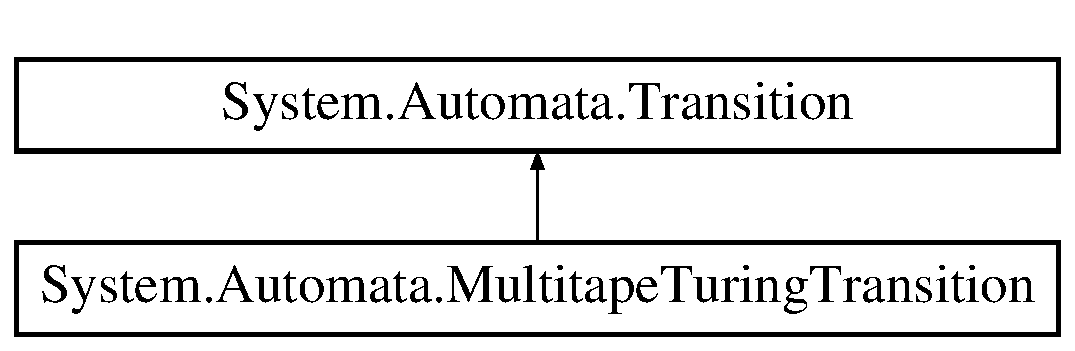
\includegraphics[height=2.000000cm]{class_system_1_1_automata_1_1_multitape_turing_transition}
\end{center}
\end{figure}
\subsection*{Public Member Functions}
\begin{DoxyCompactItemize}
\item 
\mbox{\Hypertarget{class_system_1_1_automata_1_1_multitape_turing_transition_a0f5fb925d5e90421e8e8233fb4cad694}\label{class_system_1_1_automata_1_1_multitape_turing_transition_a0f5fb925d5e90421e8e8233fb4cad694}} 
{\bfseries Multitape\+Turing\+Transition} (\mbox{\hyperlink{class_system_1_1_automata_1_1_state}{State}} p, char\mbox{[}$\,$\mbox{]} x, \mbox{\hyperlink{class_system_1_1_automata_1_1_state}{State}} q, Tuple$<$ char, \mbox{\hyperlink{class_system_1_1_automata_1_1_turing_machine_aa253c3820befa3cfdd3d17b2d8fdd2d9}{Turing\+Machine.\+Direction}} $>$\mbox{[}$\,$\mbox{]} y)
\item 
\mbox{\Hypertarget{class_system_1_1_automata_1_1_multitape_turing_transition_a2b2fdf9244fbe35e2537c56ed745b1d1}\label{class_system_1_1_automata_1_1_multitape_turing_transition_a2b2fdf9244fbe35e2537c56ed745b1d1}} 
override string {\bfseries To\+String} ()
\end{DoxyCompactItemize}
\subsection*{Properties}
\begin{DoxyCompactItemize}
\item 
Read\+Only\+Collection$<$ char $>$ \mbox{\hyperlink{class_system_1_1_automata_1_1_multitape_turing_transition_ac75736919c5dd909eda605dbb2e1a963}{Initial\+Characters}}\hspace{0.3cm}{\ttfamily  \mbox{[}get\mbox{]}}
\begin{DoxyCompactList}\small\item\em The list of current characters on each tape. \end{DoxyCompactList}\item 
Read\+Only\+Collection$<$ Tuple$<$ char, \mbox{\hyperlink{class_system_1_1_automata_1_1_turing_machine_aa253c3820befa3cfdd3d17b2d8fdd2d9}{Turing\+Machine.\+Direction}} $>$ $>$ \mbox{\hyperlink{class_system_1_1_automata_1_1_multitape_turing_transition_a448257e60c734d530225bf3770673732}{Final\+Moves}}\hspace{0.3cm}{\ttfamily  \mbox{[}get\mbox{]}}
\begin{DoxyCompactList}\small\item\em The list of moves for each tape. \end{DoxyCompactList}\end{DoxyCompactItemize}


\subsection{Detailed Description}
A transition for a Turing machine with multiple tapes. 



\subsection{Property Documentation}
\mbox{\Hypertarget{class_system_1_1_automata_1_1_multitape_turing_transition_a448257e60c734d530225bf3770673732}\label{class_system_1_1_automata_1_1_multitape_turing_transition_a448257e60c734d530225bf3770673732}} 
\index{System\+::\+Automata\+::\+Multitape\+Turing\+Transition@{System\+::\+Automata\+::\+Multitape\+Turing\+Transition}!Final\+Moves@{Final\+Moves}}
\index{Final\+Moves@{Final\+Moves}!System\+::\+Automata\+::\+Multitape\+Turing\+Transition@{System\+::\+Automata\+::\+Multitape\+Turing\+Transition}}
\subsubsection{\texorpdfstring{Final\+Moves}{FinalMoves}}
{\footnotesize\ttfamily Read\+Only\+Collection$<$Tuple$<$char, \mbox{\hyperlink{class_system_1_1_automata_1_1_turing_machine_aa253c3820befa3cfdd3d17b2d8fdd2d9}{Turing\+Machine.\+Direction}}$>$ $>$ System.\+Automata.\+Multitape\+Turing\+Transition.\+Final\+Moves\hspace{0.3cm}{\ttfamily [get]}}



The list of moves for each tape. 

\mbox{\Hypertarget{class_system_1_1_automata_1_1_multitape_turing_transition_ac75736919c5dd909eda605dbb2e1a963}\label{class_system_1_1_automata_1_1_multitape_turing_transition_ac75736919c5dd909eda605dbb2e1a963}} 
\index{System\+::\+Automata\+::\+Multitape\+Turing\+Transition@{System\+::\+Automata\+::\+Multitape\+Turing\+Transition}!Initial\+Characters@{Initial\+Characters}}
\index{Initial\+Characters@{Initial\+Characters}!System\+::\+Automata\+::\+Multitape\+Turing\+Transition@{System\+::\+Automata\+::\+Multitape\+Turing\+Transition}}
\subsubsection{\texorpdfstring{Initial\+Characters}{InitialCharacters}}
{\footnotesize\ttfamily Read\+Only\+Collection$<$char$>$ System.\+Automata.\+Multitape\+Turing\+Transition.\+Initial\+Characters\hspace{0.3cm}{\ttfamily [get]}}



The list of current characters on each tape. 



The documentation for this class was generated from the following file\+:\begin{DoxyCompactItemize}
\item 
System.\+Automata/Multitape\+Turing\+Transition.\+cs\end{DoxyCompactItemize}

\hypertarget{class_system_1_1_automata_1_1_multitape_turing_transition_function}{}\section{System.\+Automata.\+Multitape\+Turing\+Transition\+Function Class Reference}
\label{class_system_1_1_automata_1_1_multitape_turing_transition_function}\index{System.\+Automata.\+Multitape\+Turing\+Transition\+Function@{System.\+Automata.\+Multitape\+Turing\+Transition\+Function}}
Inheritance diagram for System.\+Automata.\+Multitape\+Turing\+Transition\+Function\+:\begin{figure}[H]
\begin{center}
\leavevmode
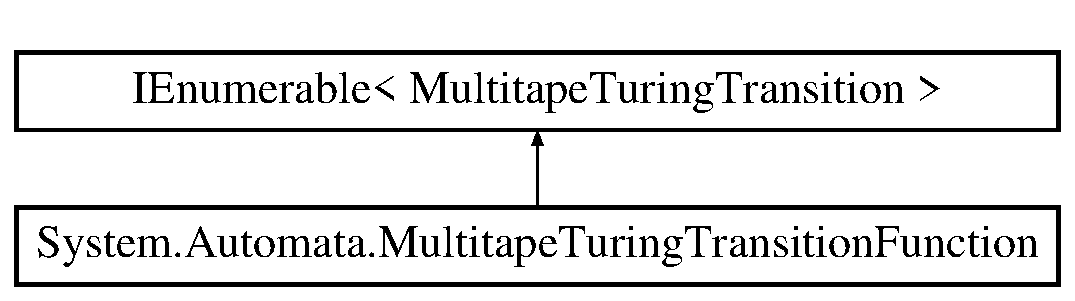
\includegraphics[height=2.000000cm]{class_system_1_1_automata_1_1_multitape_turing_transition_function}
\end{center}
\end{figure}
\subsection*{Public Member Functions}
\begin{DoxyCompactItemize}
\item 
\mbox{\Hypertarget{class_system_1_1_automata_1_1_multitape_turing_transition_function_abc2028b8c1da4d151a94e9661fc4cea3}\label{class_system_1_1_automata_1_1_multitape_turing_transition_function_abc2028b8c1da4d151a94e9661fc4cea3}} 
{\bfseries Multitape\+Turing\+Transition\+Function} (params \mbox{\hyperlink{class_system_1_1_automata_1_1_multitape_turing_transition}{Multitape\+Turing\+Transition}}\mbox{[}$\,$\mbox{]} t)
\item 
\mbox{\Hypertarget{class_system_1_1_automata_1_1_multitape_turing_transition_function_a3a0bac9d6625523730d900a1a8dbb01a}\label{class_system_1_1_automata_1_1_multitape_turing_transition_function_a3a0bac9d6625523730d900a1a8dbb01a}} 
void {\bfseries Add} (\mbox{\hyperlink{class_system_1_1_automata_1_1_multitape_turing_transition}{Multitape\+Turing\+Transition}} t)
\item 
\mbox{\Hypertarget{class_system_1_1_automata_1_1_multitape_turing_transition_function_a6b11b7337cbd5e84f087bfcda1def9b4}\label{class_system_1_1_automata_1_1_multitape_turing_transition_function_a6b11b7337cbd5e84f087bfcda1def9b4}} 
bool {\bfseries Contains} (\mbox{\hyperlink{class_system_1_1_automata_1_1_multitape_turing_transition}{Multitape\+Turing\+Transition}} t)
\item 
\mbox{\Hypertarget{class_system_1_1_automata_1_1_multitape_turing_transition_function_a2aa88815dde298242349e655000e9c91}\label{class_system_1_1_automata_1_1_multitape_turing_transition_function_a2aa88815dde298242349e655000e9c91}} 
bool {\bfseries Exists} (Predicate$<$ \mbox{\hyperlink{class_system_1_1_automata_1_1_multitape_turing_transition}{Multitape\+Turing\+Transition}} $>$ p)
\item 
\mbox{\Hypertarget{class_system_1_1_automata_1_1_multitape_turing_transition_function_a949c8706940c8bd94018b35650c42136}\label{class_system_1_1_automata_1_1_multitape_turing_transition_function_a949c8706940c8bd94018b35650c42136}} 
I\+Enumerator$<$ \mbox{\hyperlink{class_system_1_1_automata_1_1_multitape_turing_transition}{Multitape\+Turing\+Transition}} $>$ {\bfseries Get\+Enumerator} ()
\end{DoxyCompactItemize}
\subsection*{Public Attributes}
\begin{DoxyCompactItemize}
\item 
\mbox{\Hypertarget{class_system_1_1_automata_1_1_multitape_turing_transition_function_a19f2ec1f5277d8f90e9bf762d1acdc30}\label{class_system_1_1_automata_1_1_multitape_turing_transition_function_a19f2ec1f5277d8f90e9bf762d1acdc30}} 
int {\bfseries Count} =$>$ \+\_\+trans.\+Count
\item 
\mbox{\hyperlink{class_system_1_1_automata_1_1_multitape_turing_transition}{Multitape\+Turing\+Transition}} \mbox{[}$\,$\mbox{]} this\mbox{[}\mbox{\hyperlink{class_system_1_1_automata_1_1_state}{State}} p, char\mbox{[}$\,$\mbox{]} {\bfseries a}
\end{DoxyCompactItemize}


\subsection{Member Data Documentation}
\mbox{\Hypertarget{class_system_1_1_automata_1_1_multitape_turing_transition_function_a9cfbfb52eb78895705fa0b46908e55c6}\label{class_system_1_1_automata_1_1_multitape_turing_transition_function_a9cfbfb52eb78895705fa0b46908e55c6}} 
\index{System\+::\+Automata\+::\+Multitape\+Turing\+Transition\+Function@{System\+::\+Automata\+::\+Multitape\+Turing\+Transition\+Function}!a@{a}}
\index{a@{a}!System\+::\+Automata\+::\+Multitape\+Turing\+Transition\+Function@{System\+::\+Automata\+::\+Multitape\+Turing\+Transition\+Function}}
\subsubsection{\texorpdfstring{a}{a}}
{\footnotesize\ttfamily \mbox{\hyperlink{class_system_1_1_automata_1_1_multitape_turing_transition}{Multitape\+Turing\+Transition}} \mbox{[}$\,$\mbox{]} this\mbox{[}\mbox{\hyperlink{class_system_1_1_automata_1_1_state}{State}} p, char\mbox{[}$\,$\mbox{]} System.\+Automata.\+Multitape\+Turing\+Transition\+Function.\+a}

{\bfseries Initial value\+:}
\begin{DoxyCode}
=>
            \_trans.Where(x => x.P.Equals(p) && x.InitialCharacters.Count == a.Length && x.
      \mbox{\hyperlink{class_system_1_1_automata_1_1_multitape_turing_transition_ac75736919c5dd909eda605dbb2e1a963}{InitialCharacters}}.SequenceEqual(a))
                .ToArray()
\end{DoxyCode}


The documentation for this class was generated from the following file\+:\begin{DoxyCompactItemize}
\item 
System.\+Automata/Multitape\+Turing\+Transition\+Function.\+cs\end{DoxyCompactItemize}

\hypertarget{class_system_1_1_automata_1_1_nondeterministic_finite_automaton}{}\section{System.\+Automata.\+Nondeterministic\+Finite\+Automaton Class Reference}
\label{class_system_1_1_automata_1_1_nondeterministic_finite_automaton}\index{System.\+Automata.\+Nondeterministic\+Finite\+Automaton@{System.\+Automata.\+Nondeterministic\+Finite\+Automaton}}


A nondeterministic Finite \mbox{\hyperlink{class_system_1_1_automata_1_1_automaton}{Automaton}}  


Inheritance diagram for System.\+Automata.\+Nondeterministic\+Finite\+Automaton\+:\begin{figure}[H]
\begin{center}
\leavevmode
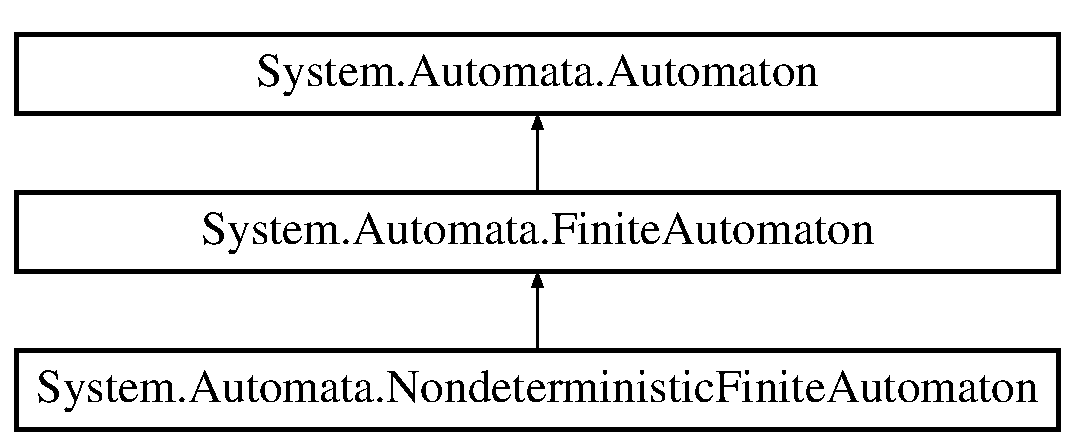
\includegraphics[height=3.000000cm]{class_system_1_1_automata_1_1_nondeterministic_finite_automaton}
\end{center}
\end{figure}
\subsection*{Public Member Functions}
\begin{DoxyCompactItemize}
\item 
\mbox{\Hypertarget{class_system_1_1_automata_1_1_nondeterministic_finite_automaton_a47356ccfa442fa648fc954a728d8af6b}\label{class_system_1_1_automata_1_1_nondeterministic_finite_automaton_a47356ccfa442fa648fc954a728d8af6b}} 
{\bfseries Nondeterministic\+Finite\+Automaton} (\mbox{\hyperlink{class_system_1_1_automata_1_1_states}{States}} q, \mbox{\hyperlink{class_system_1_1_automata_1_1_alphabet}{Alphabet}} a, \mbox{\hyperlink{class_system_1_1_automata_1_1_nondeterministic_transition_function}{Nondeterministic\+Transition\+Function}} d, \mbox{\hyperlink{class_system_1_1_automata_1_1_state}{State}} q0, \mbox{\hyperlink{class_system_1_1_automata_1_1_accepting_states}{Accepting\+States}} f)
\item 
\mbox{\Hypertarget{class_system_1_1_automata_1_1_nondeterministic_finite_automaton_a07db23e6e2c3a6e8f8268baa219a053f}\label{class_system_1_1_automata_1_1_nondeterministic_finite_automaton_a07db23e6e2c3a6e8f8268baa219a053f}} 
new bool {\bfseries Run} (char\mbox{[}$\,$\mbox{]} x)
\item 
\mbox{\Hypertarget{class_system_1_1_automata_1_1_nondeterministic_finite_automaton_a75de5d0315312f16f00c5dfd825de735}\label{class_system_1_1_automata_1_1_nondeterministic_finite_automaton_a75de5d0315312f16f00c5dfd825de735}} 
new bool {\bfseries Run} (string x)
\end{DoxyCompactItemize}
\subsection*{Properties}
\begin{DoxyCompactItemize}
\item 
new \mbox{\hyperlink{class_system_1_1_automata_1_1_nondeterministic_transition_function}{Nondeterministic\+Transition\+Function}} \mbox{\hyperlink{class_system_1_1_automata_1_1_nondeterministic_finite_automaton_ab34f2411b1591e0eb87cfde9671f4c4a}{Transitions}}\hspace{0.3cm}{\ttfamily  \mbox{[}get\mbox{]}}
\begin{DoxyCompactList}\small\item\em \mbox{\hyperlink{class_system_1_1_automata_1_1_state}{State}} transition mappings \end{DoxyCompactList}\end{DoxyCompactItemize}


\subsection{Detailed Description}
A nondeterministic Finite \mbox{\hyperlink{class_system_1_1_automata_1_1_automaton}{Automaton}} 



\subsection{Property Documentation}
\mbox{\Hypertarget{class_system_1_1_automata_1_1_nondeterministic_finite_automaton_ab34f2411b1591e0eb87cfde9671f4c4a}\label{class_system_1_1_automata_1_1_nondeterministic_finite_automaton_ab34f2411b1591e0eb87cfde9671f4c4a}} 
\index{System\+::\+Automata\+::\+Nondeterministic\+Finite\+Automaton@{System\+::\+Automata\+::\+Nondeterministic\+Finite\+Automaton}!Transitions@{Transitions}}
\index{Transitions@{Transitions}!System\+::\+Automata\+::\+Nondeterministic\+Finite\+Automaton@{System\+::\+Automata\+::\+Nondeterministic\+Finite\+Automaton}}
\subsubsection{\texorpdfstring{Transitions}{Transitions}}
{\footnotesize\ttfamily new \mbox{\hyperlink{class_system_1_1_automata_1_1_nondeterministic_transition_function}{Nondeterministic\+Transition\+Function}} System.\+Automata.\+Nondeterministic\+Finite\+Automaton.\+Transitions\hspace{0.3cm}{\ttfamily [get]}}



\mbox{\hyperlink{class_system_1_1_automata_1_1_state}{State}} transition mappings 



The documentation for this class was generated from the following file\+:\begin{DoxyCompactItemize}
\item 
System.\+Automata/Nondeterministic\+Finite\+Automaton.\+cs\end{DoxyCompactItemize}

\hypertarget{class_system_1_1_automata_1_1_nondeterministic_transition_function}{}\section{System.\+Automata.\+Nondeterministic\+Transition\+Function Class Reference}
\label{class_system_1_1_automata_1_1_nondeterministic_transition_function}\index{System.\+Automata.\+Nondeterministic\+Transition\+Function@{System.\+Automata.\+Nondeterministic\+Transition\+Function}}


A nondeterministic collection of state transition mappings.  


Inheritance diagram for System.\+Automata.\+Nondeterministic\+Transition\+Function\+:\begin{figure}[H]
\begin{center}
\leavevmode
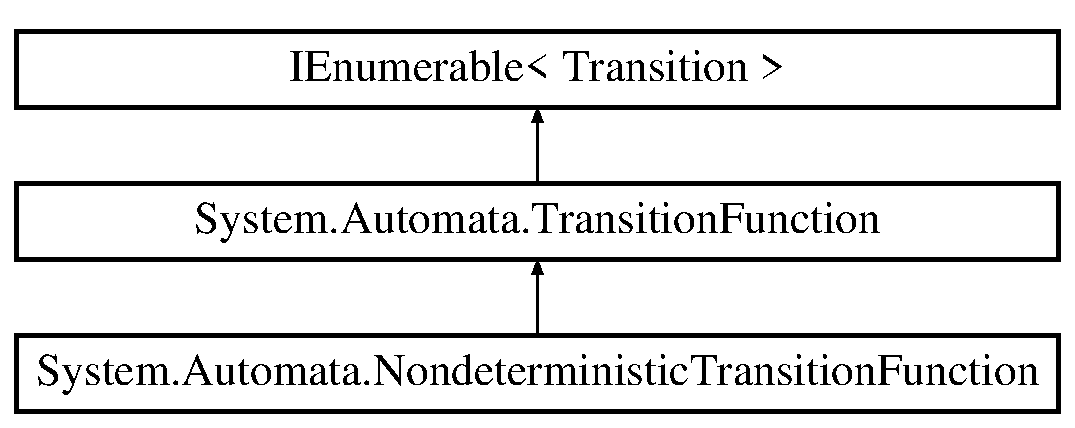
\includegraphics[height=3.000000cm]{class_system_1_1_automata_1_1_nondeterministic_transition_function}
\end{center}
\end{figure}
\subsection*{Public Member Functions}
\begin{DoxyCompactItemize}
\item 
\mbox{\Hypertarget{class_system_1_1_automata_1_1_nondeterministic_transition_function_a0099045f999ab2035909872f4e3e9594}\label{class_system_1_1_automata_1_1_nondeterministic_transition_function_a0099045f999ab2035909872f4e3e9594}} 
{\bfseries Nondeterministic\+Transition\+Function} (params \mbox{\hyperlink{class_system_1_1_automata_1_1_transition}{Transition}}\mbox{[}$\,$\mbox{]} t)
\item 
\mbox{\Hypertarget{class_system_1_1_automata_1_1_nondeterministic_transition_function_a57a2565385a005f0900b37c1b2085bfe}\label{class_system_1_1_automata_1_1_nondeterministic_transition_function_a57a2565385a005f0900b37c1b2085bfe}} 
new void {\bfseries Add} (\mbox{\hyperlink{class_system_1_1_automata_1_1_transition}{Transition}} t)
\end{DoxyCompactItemize}
\subsection*{Public Attributes}
\begin{DoxyCompactItemize}
\item 
\mbox{\Hypertarget{class_system_1_1_automata_1_1_nondeterministic_transition_function_aac5e108e3c807915075806a0788f2c97}\label{class_system_1_1_automata_1_1_nondeterministic_transition_function_aac5e108e3c807915075806a0788f2c97}} 
new \mbox{\hyperlink{class_system_1_1_automata_1_1_transition}{Transition}} \mbox{[}$\,$\mbox{]} {\bfseries this\mbox{[}\+State p, char s\mbox{]}} =$>$ Get(p, s)
\end{DoxyCompactItemize}
\subsection*{Additional Inherited Members}


\subsection{Detailed Description}
A nondeterministic collection of state transition mappings. 



The documentation for this class was generated from the following file\+:\begin{DoxyCompactItemize}
\item 
System.\+Automata/Nondeterministic\+Transition\+Function.\+cs\end{DoxyCompactItemize}

\hypertarget{class_system_1_1_automata_1_1_pushdown_automaton}{}\section{System.\+Automata.\+Pushdown\+Automaton Class Reference}
\label{class_system_1_1_automata_1_1_pushdown_automaton}\index{System.\+Automata.\+Pushdown\+Automaton@{System.\+Automata.\+Pushdown\+Automaton}}


A deterministic pushdown automaton utilizing a stack.  


Inheritance diagram for System.\+Automata.\+Pushdown\+Automaton\+:\begin{figure}[H]
\begin{center}
\leavevmode
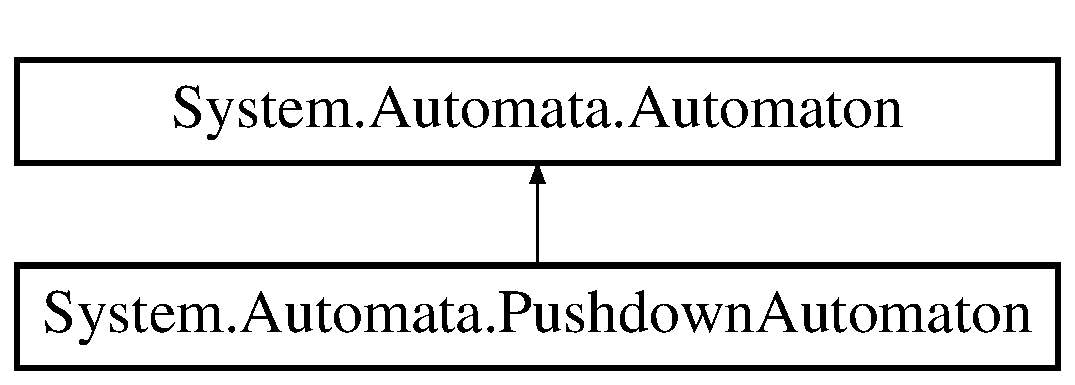
\includegraphics[height=2.000000cm]{class_system_1_1_automata_1_1_pushdown_automaton}
\end{center}
\end{figure}
\subsection*{Public Member Functions}
\begin{DoxyCompactItemize}
\item 
\mbox{\hyperlink{class_system_1_1_automata_1_1_pushdown_automaton_a5cfa8067f1080fe92500ed5eb4edf147}{Pushdown\+Automaton}} (\mbox{\hyperlink{class_system_1_1_automata_1_1_states}{States}} q, \mbox{\hyperlink{class_system_1_1_automata_1_1_alphabet}{Alphabet}} a, \mbox{\hyperlink{class_system_1_1_automata_1_1_stack_alphabet}{Stack\+Alphabet}} g, \mbox{\hyperlink{class_system_1_1_automata_1_1_pushdown_transition_function}{Pushdown\+Transition\+Function}} d, \mbox{\hyperlink{class_system_1_1_automata_1_1_state}{State}} q0, \mbox{\hyperlink{class_system_1_1_automata_1_1_accepting_states}{Accepting\+States}} f)
\item 
\mbox{\Hypertarget{class_system_1_1_automata_1_1_pushdown_automaton_ad54cf243b35b8991faa785678e1f069a}\label{class_system_1_1_automata_1_1_pushdown_automaton_ad54cf243b35b8991faa785678e1f069a}} 
bool {\bfseries Run} (char\mbox{[}$\,$\mbox{]} x)
\item 
\mbox{\Hypertarget{class_system_1_1_automata_1_1_pushdown_automaton_a4d60ea20931e7b80526ce0105d9b667a}\label{class_system_1_1_automata_1_1_pushdown_automaton_a4d60ea20931e7b80526ce0105d9b667a}} 
bool {\bfseries Run} (string x)
\end{DoxyCompactItemize}
\subsection*{Properties}
\begin{DoxyCompactItemize}
\item 
\mbox{\hyperlink{class_system_1_1_automata_1_1_stack_alphabet}{Stack\+Alphabet}} \mbox{\hyperlink{class_system_1_1_automata_1_1_pushdown_automaton_ac6e0b6accb2e2da48f0d6b4179714e15}{Stack\+Alphabet}}\hspace{0.3cm}{\ttfamily  \mbox{[}get\mbox{]}}
\begin{DoxyCompactList}\small\item\em The stack alphabet. \end{DoxyCompactList}\item 
new \mbox{\hyperlink{class_system_1_1_automata_1_1_pushdown_transition_function}{Pushdown\+Transition\+Function}} \mbox{\hyperlink{class_system_1_1_automata_1_1_pushdown_automaton_a2f4b67078bb3b628ff512fc5db396269}{Transitions}}\hspace{0.3cm}{\ttfamily  \mbox{[}get\mbox{]}}
\begin{DoxyCompactList}\small\item\em The transition function \end{DoxyCompactList}\end{DoxyCompactItemize}


\subsection{Detailed Description}
A deterministic pushdown automaton utilizing a stack. 



\subsection{Constructor \& Destructor Documentation}
\mbox{\Hypertarget{class_system_1_1_automata_1_1_pushdown_automaton_a5cfa8067f1080fe92500ed5eb4edf147}\label{class_system_1_1_automata_1_1_pushdown_automaton_a5cfa8067f1080fe92500ed5eb4edf147}} 
\index{System\+::\+Automata\+::\+Pushdown\+Automaton@{System\+::\+Automata\+::\+Pushdown\+Automaton}!Pushdown\+Automaton@{Pushdown\+Automaton}}
\index{Pushdown\+Automaton@{Pushdown\+Automaton}!System\+::\+Automata\+::\+Pushdown\+Automaton@{System\+::\+Automata\+::\+Pushdown\+Automaton}}
\subsubsection{\texorpdfstring{Pushdown\+Automaton()}{PushdownAutomaton()}}
{\footnotesize\ttfamily System.\+Automata.\+Pushdown\+Automaton.\+Pushdown\+Automaton (\begin{DoxyParamCaption}\item[{\mbox{\hyperlink{class_system_1_1_automata_1_1_states}{States}}}]{q,  }\item[{\mbox{\hyperlink{class_system_1_1_automata_1_1_alphabet}{Alphabet}}}]{a,  }\item[{\mbox{\hyperlink{class_system_1_1_automata_1_1_stack_alphabet}{Stack\+Alphabet}}}]{g,  }\item[{\mbox{\hyperlink{class_system_1_1_automata_1_1_pushdown_transition_function}{Pushdown\+Transition\+Function}}}]{d,  }\item[{\mbox{\hyperlink{class_system_1_1_automata_1_1_state}{State}}}]{q0,  }\item[{\mbox{\hyperlink{class_system_1_1_automata_1_1_accepting_states}{Accepting\+States}}}]{f }\end{DoxyParamCaption})}


\begin{DoxyParams}{Parameters}
{\em q} & The set of states\\
\hline
{\em a} & The language alphabet\\
\hline
{\em g} & The stack alphabet\\
\hline
{\em d} & The transition function containing \mbox{\hyperlink{class_system_1_1_automata_1_1_transition}{Transition}} and \mbox{\hyperlink{class_system_1_1_automata_1_1_pushdown_transition}{Pushdown\+Transition}} objects\\
\hline
{\em q0} & The initial state\\
\hline
{\em f} & The set of accepting states\\
\hline
\end{DoxyParams}

\begin{DoxyExceptions}{Exceptions}
{\em Argument\+Exception} & \\
\hline
\end{DoxyExceptions}


\subsection{Property Documentation}
\mbox{\Hypertarget{class_system_1_1_automata_1_1_pushdown_automaton_ac6e0b6accb2e2da48f0d6b4179714e15}\label{class_system_1_1_automata_1_1_pushdown_automaton_ac6e0b6accb2e2da48f0d6b4179714e15}} 
\index{System\+::\+Automata\+::\+Pushdown\+Automaton@{System\+::\+Automata\+::\+Pushdown\+Automaton}!Stack\+Alphabet@{Stack\+Alphabet}}
\index{Stack\+Alphabet@{Stack\+Alphabet}!System\+::\+Automata\+::\+Pushdown\+Automaton@{System\+::\+Automata\+::\+Pushdown\+Automaton}}
\subsubsection{\texorpdfstring{Stack\+Alphabet}{StackAlphabet}}
{\footnotesize\ttfamily \mbox{\hyperlink{class_system_1_1_automata_1_1_stack_alphabet}{Stack\+Alphabet}} System.\+Automata.\+Pushdown\+Automaton.\+Stack\+Alphabet\hspace{0.3cm}{\ttfamily [get]}}



The stack alphabet. 

\mbox{\Hypertarget{class_system_1_1_automata_1_1_pushdown_automaton_a2f4b67078bb3b628ff512fc5db396269}\label{class_system_1_1_automata_1_1_pushdown_automaton_a2f4b67078bb3b628ff512fc5db396269}} 
\index{System\+::\+Automata\+::\+Pushdown\+Automaton@{System\+::\+Automata\+::\+Pushdown\+Automaton}!Transitions@{Transitions}}
\index{Transitions@{Transitions}!System\+::\+Automata\+::\+Pushdown\+Automaton@{System\+::\+Automata\+::\+Pushdown\+Automaton}}
\subsubsection{\texorpdfstring{Transitions}{Transitions}}
{\footnotesize\ttfamily new \mbox{\hyperlink{class_system_1_1_automata_1_1_pushdown_transition_function}{Pushdown\+Transition\+Function}} System.\+Automata.\+Pushdown\+Automaton.\+Transitions\hspace{0.3cm}{\ttfamily [get]}}



The transition function 



The documentation for this class was generated from the following file\+:\begin{DoxyCompactItemize}
\item 
System.\+Automata/Pushdown\+Automaton.\+cs\end{DoxyCompactItemize}

\hypertarget{class_system_1_1_automata_1_1_pushdown_transition}{}\section{System.\+Automata.\+Pushdown\+Transition Class Reference}
\label{class_system_1_1_automata_1_1_pushdown_transition}\index{System.\+Automata.\+Pushdown\+Transition@{System.\+Automata.\+Pushdown\+Transition}}
Inheritance diagram for System.\+Automata.\+Pushdown\+Transition\+:\begin{figure}[H]
\begin{center}
\leavevmode
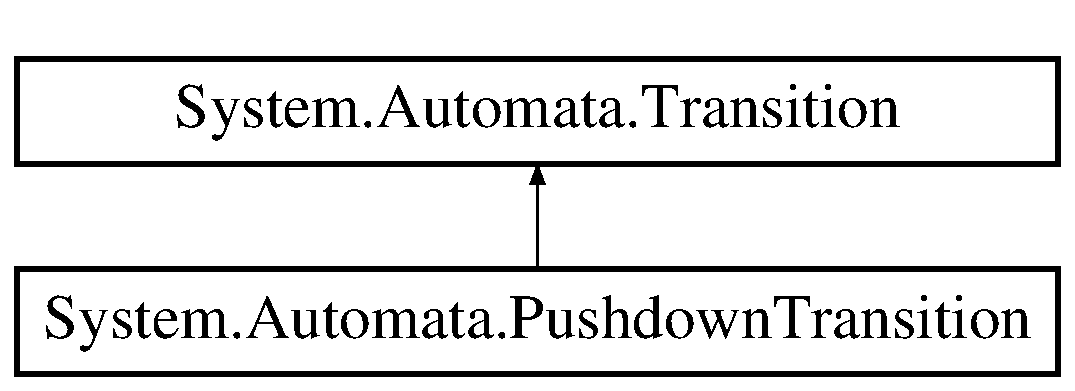
\includegraphics[height=2.000000cm]{class_system_1_1_automata_1_1_pushdown_transition}
\end{center}
\end{figure}
\subsection*{Public Member Functions}
\begin{DoxyCompactItemize}
\item 
\mbox{\Hypertarget{class_system_1_1_automata_1_1_pushdown_transition_afc1ee3b1685d5de0afdd765d0257420a}\label{class_system_1_1_automata_1_1_pushdown_transition_afc1ee3b1685d5de0afdd765d0257420a}} 
{\bfseries Pushdown\+Transition} (\mbox{\hyperlink{class_system_1_1_automata_1_1_state}{State}} p, char a, char s, \mbox{\hyperlink{class_system_1_1_automata_1_1_state}{State}} q, char\mbox{[}$\,$\mbox{]} alpha)
\item 
\mbox{\Hypertarget{class_system_1_1_automata_1_1_pushdown_transition_a093f85093482d2a37a08c87bc01d5c96}\label{class_system_1_1_automata_1_1_pushdown_transition_a093f85093482d2a37a08c87bc01d5c96}} 
{\bfseries Pushdown\+Transition} (\mbox{\hyperlink{class_system_1_1_automata_1_1_state}{State}} p, char a, char s, \mbox{\hyperlink{class_system_1_1_automata_1_1_state}{State}} q, string alpha)
\item 
\mbox{\Hypertarget{class_system_1_1_automata_1_1_pushdown_transition_ac0cf59a17fa2365c0d1755c609af948a}\label{class_system_1_1_automata_1_1_pushdown_transition_ac0cf59a17fa2365c0d1755c609af948a}} 
override string {\bfseries To\+String} ()
\end{DoxyCompactItemize}
\subsection*{Properties}
\begin{DoxyCompactItemize}
\item 
char \mbox{\hyperlink{class_system_1_1_automata_1_1_pushdown_transition_a956fe648291a21855c2d151668fd2411}{Top}}\hspace{0.3cm}{\ttfamily  \mbox{[}get\mbox{]}}
\begin{DoxyCompactList}\small\item\em The top stack character \end{DoxyCompactList}\item 
char \mbox{[}$\,$\mbox{]} \mbox{\hyperlink{class_system_1_1_automata_1_1_pushdown_transition_a8294a0ad226f3594492792271d178e06}{Replace}}\hspace{0.3cm}{\ttfamily  \mbox{[}get\mbox{]}}
\begin{DoxyCompactList}\small\item\em The sequence to replace the top stack character with. Use \mbox{\hyperlink{class_system_1_1_automata_1_1_alphabet_aa3f8c16de4596ed24f2fe0fb77e7493c}{Alphabet.\+Empty\+String}} to delete the top stack character. \end{DoxyCompactList}\end{DoxyCompactItemize}


\subsection{Property Documentation}
\mbox{\Hypertarget{class_system_1_1_automata_1_1_pushdown_transition_a8294a0ad226f3594492792271d178e06}\label{class_system_1_1_automata_1_1_pushdown_transition_a8294a0ad226f3594492792271d178e06}} 
\index{System\+::\+Automata\+::\+Pushdown\+Transition@{System\+::\+Automata\+::\+Pushdown\+Transition}!Replace@{Replace}}
\index{Replace@{Replace}!System\+::\+Automata\+::\+Pushdown\+Transition@{System\+::\+Automata\+::\+Pushdown\+Transition}}
\subsubsection{\texorpdfstring{Replace}{Replace}}
{\footnotesize\ttfamily char \mbox{[}$\,$\mbox{]} System.\+Automata.\+Pushdown\+Transition.\+Replace\hspace{0.3cm}{\ttfamily [get]}}



The sequence to replace the top stack character with. Use \mbox{\hyperlink{class_system_1_1_automata_1_1_alphabet_aa3f8c16de4596ed24f2fe0fb77e7493c}{Alphabet.\+Empty\+String}} to delete the top stack character. 

\mbox{\Hypertarget{class_system_1_1_automata_1_1_pushdown_transition_a956fe648291a21855c2d151668fd2411}\label{class_system_1_1_automata_1_1_pushdown_transition_a956fe648291a21855c2d151668fd2411}} 
\index{System\+::\+Automata\+::\+Pushdown\+Transition@{System\+::\+Automata\+::\+Pushdown\+Transition}!Top@{Top}}
\index{Top@{Top}!System\+::\+Automata\+::\+Pushdown\+Transition@{System\+::\+Automata\+::\+Pushdown\+Transition}}
\subsubsection{\texorpdfstring{Top}{Top}}
{\footnotesize\ttfamily char System.\+Automata.\+Pushdown\+Transition.\+Top\hspace{0.3cm}{\ttfamily [get]}}



The top stack character 



The documentation for this class was generated from the following file\+:\begin{DoxyCompactItemize}
\item 
System.\+Automata/Pushdown\+Transition.\+cs\end{DoxyCompactItemize}

\hypertarget{class_system_1_1_automata_1_1_pushdown_transition_function}{}\section{System.\+Automata.\+Pushdown\+Transition\+Function Class Reference}
\label{class_system_1_1_automata_1_1_pushdown_transition_function}\index{System.\+Automata.\+Pushdown\+Transition\+Function@{System.\+Automata.\+Pushdown\+Transition\+Function}}


A collection of state transition mappings for P\+D\+As  


Inheritance diagram for System.\+Automata.\+Pushdown\+Transition\+Function\+:\begin{figure}[H]
\begin{center}
\leavevmode
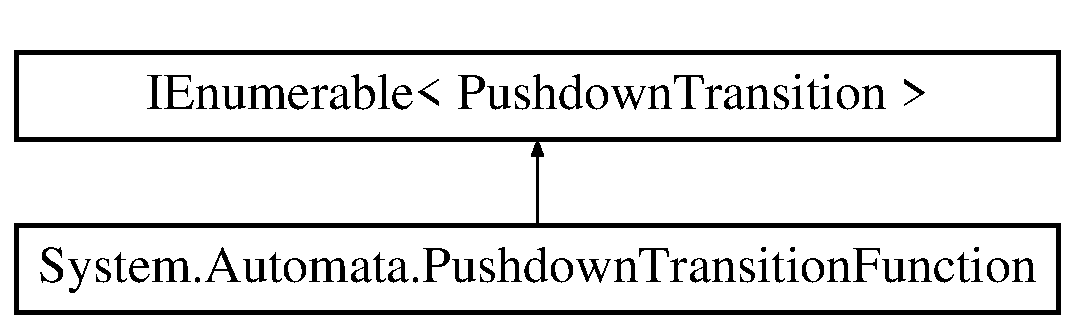
\includegraphics[height=2.000000cm]{class_system_1_1_automata_1_1_pushdown_transition_function}
\end{center}
\end{figure}
\subsection*{Public Member Functions}
\begin{DoxyCompactItemize}
\item 
\mbox{\Hypertarget{class_system_1_1_automata_1_1_pushdown_transition_function_a2f4c35d7442e155bf73aaa70c3bb203e}\label{class_system_1_1_automata_1_1_pushdown_transition_function_a2f4c35d7442e155bf73aaa70c3bb203e}} 
{\bfseries Pushdown\+Transition\+Function} (params \mbox{\hyperlink{class_system_1_1_automata_1_1_pushdown_transition}{Pushdown\+Transition}}\mbox{[}$\,$\mbox{]} t)
\item 
\mbox{\Hypertarget{class_system_1_1_automata_1_1_pushdown_transition_function_a2f391f47af647521368f76797263e999}\label{class_system_1_1_automata_1_1_pushdown_transition_function_a2f391f47af647521368f76797263e999}} 
void {\bfseries Add} (\mbox{\hyperlink{class_system_1_1_automata_1_1_pushdown_transition}{Pushdown\+Transition}} t)
\item 
\mbox{\Hypertarget{class_system_1_1_automata_1_1_pushdown_transition_function_a4e7f49843ec7c016057b020f3cbc4efa}\label{class_system_1_1_automata_1_1_pushdown_transition_function_a4e7f49843ec7c016057b020f3cbc4efa}} 
bool {\bfseries Contains} (\mbox{\hyperlink{class_system_1_1_automata_1_1_pushdown_transition}{Pushdown\+Transition}} t)
\item 
\mbox{\Hypertarget{class_system_1_1_automata_1_1_pushdown_transition_function_ac1d0852a760decb8af403e01c00645d6}\label{class_system_1_1_automata_1_1_pushdown_transition_function_ac1d0852a760decb8af403e01c00645d6}} 
bool {\bfseries Exists} (Predicate$<$ \mbox{\hyperlink{class_system_1_1_automata_1_1_transition}{Transition}} $>$ p)
\item 
\mbox{\Hypertarget{class_system_1_1_automata_1_1_pushdown_transition_function_a517ca0177583fc9438b1b688d26ddacb}\label{class_system_1_1_automata_1_1_pushdown_transition_function_a517ca0177583fc9438b1b688d26ddacb}} 
I\+Enumerator$<$ \mbox{\hyperlink{class_system_1_1_automata_1_1_pushdown_transition}{Pushdown\+Transition}} $>$ {\bfseries Get\+Enumerator} ()
\end{DoxyCompactItemize}
\subsection*{Public Attributes}
\begin{DoxyCompactItemize}
\item 
\mbox{\Hypertarget{class_system_1_1_automata_1_1_pushdown_transition_function_ad889b934b944ce5d2f36afc16a1e28a2}\label{class_system_1_1_automata_1_1_pushdown_transition_function_ad889b934b944ce5d2f36afc16a1e28a2}} 
int {\bfseries Count} =$>$ \+\_\+trans.\+Count
\item 
\mbox{\hyperlink{class_system_1_1_automata_1_1_pushdown_transition}{Pushdown\+Transition}} \mbox{[}$\,$\mbox{]} {\bfseries this\mbox{[}\+State p, char a, char alpha\mbox{]}}
\end{DoxyCompactItemize}


\subsection{Detailed Description}
A collection of state transition mappings for P\+D\+As 



\subsection{Member Data Documentation}
\mbox{\Hypertarget{class_system_1_1_automata_1_1_pushdown_transition_function_ae1c7ef36c2a602d2fdce4ea41573543c}\label{class_system_1_1_automata_1_1_pushdown_transition_function_ae1c7ef36c2a602d2fdce4ea41573543c}} 
\index{System\+::\+Automata\+::\+Pushdown\+Transition\+Function@{System\+::\+Automata\+::\+Pushdown\+Transition\+Function}!this\mbox{[}\+State p, char a, char alpha\mbox{]}@{this[State p, char a, char alpha]}}
\index{this\mbox{[}\+State p, char a, char alpha\mbox{]}@{this[State p, char a, char alpha]}!System\+::\+Automata\+::\+Pushdown\+Transition\+Function@{System\+::\+Automata\+::\+Pushdown\+Transition\+Function}}
\subsubsection{\texorpdfstring{this[State p, char a, char alpha]}{this[State p, char a, char alpha]}}
{\footnotesize\ttfamily \mbox{\hyperlink{class_system_1_1_automata_1_1_pushdown_transition}{Pushdown\+Transition}} \mbox{[}$\,$\mbox{]} System.\+Automata.\+Pushdown\+Transition\+Function.\+this\mbox{[}\mbox{\hyperlink{class_system_1_1_automata_1_1_state}{State}} p, char a, char alpha\mbox{]}}

{\bfseries Initial value\+:}
\begin{DoxyCode}
=>
            \_trans.Where(x => x.P.Equals(p) && x.A == a && (x.Top == alpha || x.Top == Alphabet.Wildcard)).
      ToArray()
\end{DoxyCode}


The documentation for this class was generated from the following file\+:\begin{DoxyCompactItemize}
\item 
System.\+Automata/Pushdown\+Transition\+Function.\+cs\end{DoxyCompactItemize}

\hypertarget{class_system_1_1_automata_1_1_stack_alphabet}{}\section{System.\+Automata.\+Stack\+Alphabet Class Reference}
\label{class_system_1_1_automata_1_1_stack_alphabet}\index{System.\+Automata.\+Stack\+Alphabet@{System.\+Automata.\+Stack\+Alphabet}}


An alphabet for use with a pushdown stack  


Inheritance diagram for System.\+Automata.\+Stack\+Alphabet\+:\begin{figure}[H]
\begin{center}
\leavevmode
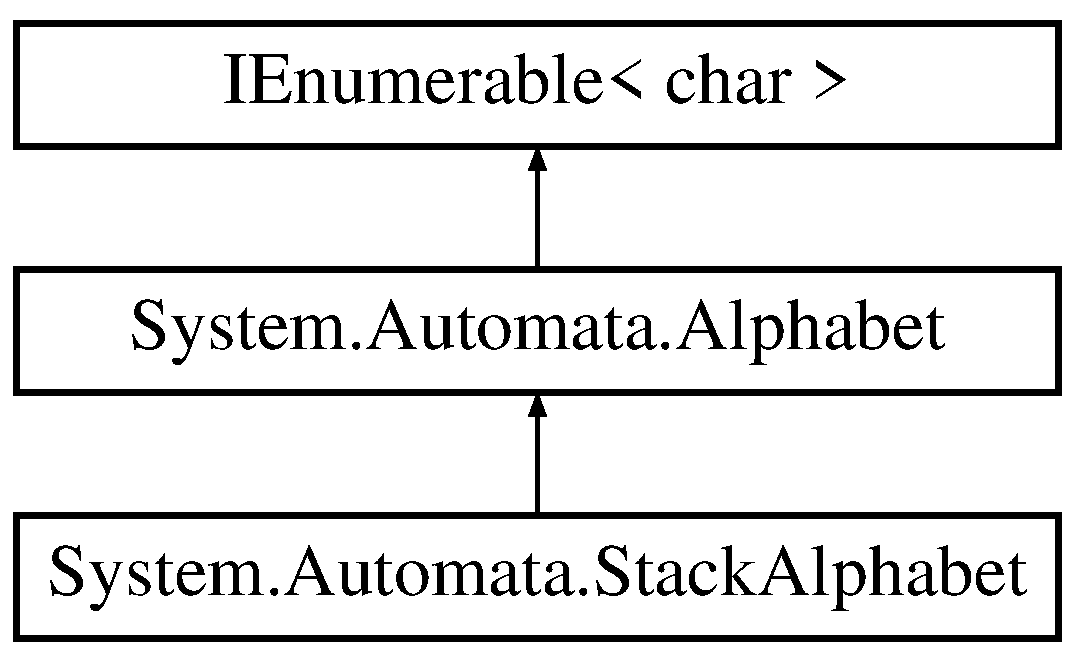
\includegraphics[height=3.000000cm]{class_system_1_1_automata_1_1_stack_alphabet}
\end{center}
\end{figure}
\subsection*{Public Member Functions}
\begin{DoxyCompactItemize}
\item 
\mbox{\Hypertarget{class_system_1_1_automata_1_1_stack_alphabet_a515e787649e8cddad7fbe3d739d313d9}\label{class_system_1_1_automata_1_1_stack_alphabet_a515e787649e8cddad7fbe3d739d313d9}} 
{\bfseries Stack\+Alphabet} (\mbox{\hyperlink{class_system_1_1_automata_1_1_alphabet}{Alphabet}} a, params char\mbox{[}$\,$\mbox{]} c)
\item 
\mbox{\Hypertarget{class_system_1_1_automata_1_1_stack_alphabet_a2cdeffdd37d35c216236ae9e33f5b532}\label{class_system_1_1_automata_1_1_stack_alphabet_a2cdeffdd37d35c216236ae9e33f5b532}} 
{\bfseries Stack\+Alphabet} (params char\mbox{[}$\,$\mbox{]} c)
\end{DoxyCompactItemize}
\subsection*{Static Public Member Functions}
\begin{DoxyCompactItemize}
\item 
\mbox{\Hypertarget{class_system_1_1_automata_1_1_stack_alphabet_a412eab1ea39abe20a9ca04737f0797fa}\label{class_system_1_1_automata_1_1_stack_alphabet_a412eab1ea39abe20a9ca04737f0797fa}} 
static \mbox{\hyperlink{class_system_1_1_automata_1_1_stack_alphabet}{Stack\+Alphabet}} {\bfseries operator+} (\mbox{\hyperlink{class_system_1_1_automata_1_1_stack_alphabet}{Stack\+Alphabet}} a, \mbox{\hyperlink{class_system_1_1_automata_1_1_alphabet}{Alphabet}} b)
\item 
\mbox{\Hypertarget{class_system_1_1_automata_1_1_stack_alphabet_a8d601a55a26b55ebec95923cb1a09b4d}\label{class_system_1_1_automata_1_1_stack_alphabet_a8d601a55a26b55ebec95923cb1a09b4d}} 
static \mbox{\hyperlink{class_system_1_1_automata_1_1_stack_alphabet}{Stack\+Alphabet}} {\bfseries operator+} (\mbox{\hyperlink{class_system_1_1_automata_1_1_alphabet}{Alphabet}} a, \mbox{\hyperlink{class_system_1_1_automata_1_1_stack_alphabet}{Stack\+Alphabet}} b)
\item 
\mbox{\Hypertarget{class_system_1_1_automata_1_1_stack_alphabet_af9c04cb6f1bc03a4116d51809155c6d1}\label{class_system_1_1_automata_1_1_stack_alphabet_af9c04cb6f1bc03a4116d51809155c6d1}} 
static \mbox{\hyperlink{class_system_1_1_automata_1_1_stack_alphabet}{Stack\+Alphabet}} {\bfseries operator+} (\mbox{\hyperlink{class_system_1_1_automata_1_1_stack_alphabet}{Stack\+Alphabet}} a, \mbox{\hyperlink{class_system_1_1_automata_1_1_stack_alphabet}{Stack\+Alphabet}} b)
\item 
\mbox{\Hypertarget{class_system_1_1_automata_1_1_stack_alphabet_afba4784c5a0fff4cffa91e556d4c627d}\label{class_system_1_1_automata_1_1_stack_alphabet_afba4784c5a0fff4cffa91e556d4c627d}} 
static \mbox{\hyperlink{class_system_1_1_automata_1_1_stack_alphabet}{Stack\+Alphabet}} {\bfseries operator-\/} (\mbox{\hyperlink{class_system_1_1_automata_1_1_stack_alphabet}{Stack\+Alphabet}} a, \mbox{\hyperlink{class_system_1_1_automata_1_1_alphabet}{Alphabet}} b)
\item 
\mbox{\Hypertarget{class_system_1_1_automata_1_1_stack_alphabet_a3490921d02545fd58b09db8858615ba1}\label{class_system_1_1_automata_1_1_stack_alphabet_a3490921d02545fd58b09db8858615ba1}} 
static \mbox{\hyperlink{class_system_1_1_automata_1_1_alphabet}{Alphabet}} {\bfseries operator-\/} (\mbox{\hyperlink{class_system_1_1_automata_1_1_alphabet}{Alphabet}} a, \mbox{\hyperlink{class_system_1_1_automata_1_1_stack_alphabet}{Stack\+Alphabet}} b)
\item 
\mbox{\Hypertarget{class_system_1_1_automata_1_1_stack_alphabet_a5b00d97a65b87e31b2b32762289a086f}\label{class_system_1_1_automata_1_1_stack_alphabet_a5b00d97a65b87e31b2b32762289a086f}} 
static \mbox{\hyperlink{class_system_1_1_automata_1_1_stack_alphabet}{Stack\+Alphabet}} {\bfseries operator-\/} (\mbox{\hyperlink{class_system_1_1_automata_1_1_stack_alphabet}{Stack\+Alphabet}} a, \mbox{\hyperlink{class_system_1_1_automata_1_1_stack_alphabet}{Stack\+Alphabet}} b)
\end{DoxyCompactItemize}
\subsection*{Additional Inherited Members}


\subsection{Detailed Description}
An alphabet for use with a pushdown stack 



The documentation for this class was generated from the following file\+:\begin{DoxyCompactItemize}
\item 
System.\+Automata/Stack\+Alphabet.\+cs\end{DoxyCompactItemize}

\hypertarget{class_system_1_1_automata_1_1_state}{}\section{System.\+Automata.\+State Class Reference}
\label{class_system_1_1_automata_1_1_state}\index{System.\+Automata.\+State@{System.\+Automata.\+State}}


A automaton state.  


\subsection*{Public Member Functions}
\begin{DoxyCompactItemize}
\item 
\mbox{\Hypertarget{class_system_1_1_automata_1_1_state_a6e1833f9d456c0badab1ebc2dd3f9025}\label{class_system_1_1_automata_1_1_state_a6e1833f9d456c0badab1ebc2dd3f9025}} 
\mbox{\hyperlink{class_system_1_1_automata_1_1_state_a6e1833f9d456c0badab1ebc2dd3f9025}{State}} (string name)
\begin{DoxyCompactList}\small\item\em 
\begin{DoxyParams}{Parameters}
{\em name} & The name of the state\\
\hline
\end{DoxyParams}
\end{DoxyCompactList}\item 
\mbox{\Hypertarget{class_system_1_1_automata_1_1_state_aea35e79d24a3f3e90dcc1ced6fbd3d01}\label{class_system_1_1_automata_1_1_state_aea35e79d24a3f3e90dcc1ced6fbd3d01}} 
{\bfseries State} (int id)
\item 
\mbox{\Hypertarget{class_system_1_1_automata_1_1_state_a0a0e694af6779817fa041051e696211d}\label{class_system_1_1_automata_1_1_state_a0a0e694af6779817fa041051e696211d}} 
override string {\bfseries To\+String} ()
\item 
\mbox{\Hypertarget{class_system_1_1_automata_1_1_state_afa96677a72c07d002a4a775ed855db41}\label{class_system_1_1_automata_1_1_state_afa96677a72c07d002a4a775ed855db41}} 
override bool {\bfseries Equals} (object obj)
\item 
\mbox{\Hypertarget{class_system_1_1_automata_1_1_state_ad125b073a92a6aa475abdebaf9b84e4b}\label{class_system_1_1_automata_1_1_state_ad125b073a92a6aa475abdebaf9b84e4b}} 
bool {\bfseries Equals} (\mbox{\hyperlink{class_system_1_1_automata_1_1_state}{State}} s)
\item 
\mbox{\Hypertarget{class_system_1_1_automata_1_1_state_a36f73edad3f050e26a4df64d82322587}\label{class_system_1_1_automata_1_1_state_a36f73edad3f050e26a4df64d82322587}} 
override int {\bfseries Get\+Hash\+Code} ()
\end{DoxyCompactItemize}
\subsection*{Static Public Attributes}
\begin{DoxyCompactItemize}
\item 
static readonly \mbox{\hyperlink{class_system_1_1_automata_1_1_state}{State}} \mbox{\hyperlink{class_system_1_1_automata_1_1_state_adb68e0dc49813e402e113d26e7137660}{Hr}} = new \mbox{\hyperlink{class_system_1_1_automata_1_1_state}{State}}(\char`\"{}Hr\char`\"{}) \{ Accepting = true\}
\begin{DoxyCompactList}\small\item\em The Turing halting accept state. \end{DoxyCompactList}\item 
static readonly \mbox{\hyperlink{class_system_1_1_automata_1_1_state}{State}} \mbox{\hyperlink{class_system_1_1_automata_1_1_state_ae6639cebabe973cfa8825fedbc4ae741}{Ha}} = new \mbox{\hyperlink{class_system_1_1_automata_1_1_state}{State}}(\char`\"{}Ha\char`\"{})
\begin{DoxyCompactList}\small\item\em The Turing halting reject state. \end{DoxyCompactList}\end{DoxyCompactItemize}
\subsection*{Properties}
\begin{DoxyCompactItemize}
\item 
string \mbox{\hyperlink{class_system_1_1_automata_1_1_state_aba020a3d9150baf1bfd6dd27c93cf297}{Name}}\hspace{0.3cm}{\ttfamily  \mbox{[}get\mbox{]}}
\begin{DoxyCompactList}\small\item\em The name of the state \end{DoxyCompactList}\item 
bool \mbox{\hyperlink{class_system_1_1_automata_1_1_state_a2a37b025bd8bf30defe28ae26e339e0e}{Accepting}}\hspace{0.3cm}{\ttfamily  \mbox{[}get, set\mbox{]}}
\begin{DoxyCompactList}\small\item\em Is the state an accepting state? \end{DoxyCompactList}\end{DoxyCompactItemize}


\subsection{Detailed Description}
A automaton state. 



\subsection{Member Data Documentation}
\mbox{\Hypertarget{class_system_1_1_automata_1_1_state_ae6639cebabe973cfa8825fedbc4ae741}\label{class_system_1_1_automata_1_1_state_ae6639cebabe973cfa8825fedbc4ae741}} 
\index{System\+::\+Automata\+::\+State@{System\+::\+Automata\+::\+State}!Ha@{Ha}}
\index{Ha@{Ha}!System\+::\+Automata\+::\+State@{System\+::\+Automata\+::\+State}}
\subsubsection{\texorpdfstring{Ha}{Ha}}
{\footnotesize\ttfamily readonly \mbox{\hyperlink{class_system_1_1_automata_1_1_state}{State}} System.\+Automata.\+State.\+Ha = new \mbox{\hyperlink{class_system_1_1_automata_1_1_state}{State}}(\char`\"{}Ha\char`\"{})\hspace{0.3cm}{\ttfamily [static]}}



The Turing halting reject state. 

\mbox{\Hypertarget{class_system_1_1_automata_1_1_state_adb68e0dc49813e402e113d26e7137660}\label{class_system_1_1_automata_1_1_state_adb68e0dc49813e402e113d26e7137660}} 
\index{System\+::\+Automata\+::\+State@{System\+::\+Automata\+::\+State}!Hr@{Hr}}
\index{Hr@{Hr}!System\+::\+Automata\+::\+State@{System\+::\+Automata\+::\+State}}
\subsubsection{\texorpdfstring{Hr}{Hr}}
{\footnotesize\ttfamily readonly \mbox{\hyperlink{class_system_1_1_automata_1_1_state}{State}} System.\+Automata.\+State.\+Hr = new \mbox{\hyperlink{class_system_1_1_automata_1_1_state}{State}}(\char`\"{}Hr\char`\"{}) \{ Accepting = true\}\hspace{0.3cm}{\ttfamily [static]}}



The Turing halting accept state. 



\subsection{Property Documentation}
\mbox{\Hypertarget{class_system_1_1_automata_1_1_state_a2a37b025bd8bf30defe28ae26e339e0e}\label{class_system_1_1_automata_1_1_state_a2a37b025bd8bf30defe28ae26e339e0e}} 
\index{System\+::\+Automata\+::\+State@{System\+::\+Automata\+::\+State}!Accepting@{Accepting}}
\index{Accepting@{Accepting}!System\+::\+Automata\+::\+State@{System\+::\+Automata\+::\+State}}
\subsubsection{\texorpdfstring{Accepting}{Accepting}}
{\footnotesize\ttfamily bool System.\+Automata.\+State.\+Accepting\hspace{0.3cm}{\ttfamily [get]}, {\ttfamily [set]}}



Is the state an accepting state? 

\mbox{\Hypertarget{class_system_1_1_automata_1_1_state_aba020a3d9150baf1bfd6dd27c93cf297}\label{class_system_1_1_automata_1_1_state_aba020a3d9150baf1bfd6dd27c93cf297}} 
\index{System\+::\+Automata\+::\+State@{System\+::\+Automata\+::\+State}!Name@{Name}}
\index{Name@{Name}!System\+::\+Automata\+::\+State@{System\+::\+Automata\+::\+State}}
\subsubsection{\texorpdfstring{Name}{Name}}
{\footnotesize\ttfamily string System.\+Automata.\+State.\+Name\hspace{0.3cm}{\ttfamily [get]}}



The name of the state 



The documentation for this class was generated from the following file\+:\begin{DoxyCompactItemize}
\item 
System.\+Automata/State.\+cs\end{DoxyCompactItemize}

\hypertarget{class_system_1_1_automata_1_1_states}{}\section{System.\+Automata.\+States Class Reference}
\label{class_system_1_1_automata_1_1_states}\index{System.\+Automata.\+States@{System.\+Automata.\+States}}


The set of all states  


Inheritance diagram for System.\+Automata.\+States\+:\begin{figure}[H]
\begin{center}
\leavevmode
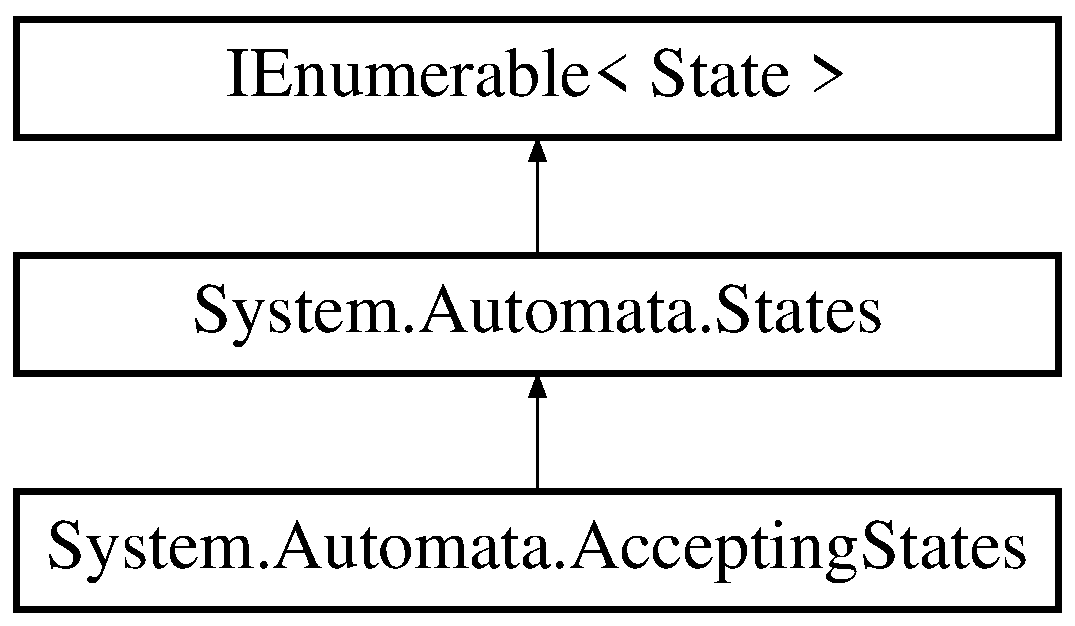
\includegraphics[height=3.000000cm]{class_system_1_1_automata_1_1_states}
\end{center}
\end{figure}
\subsection*{Public Member Functions}
\begin{DoxyCompactItemize}
\item 
\mbox{\hyperlink{class_system_1_1_automata_1_1_states_a850e135e490c7054d909453e6797ffb7}{States}} (int n)
\begin{DoxyCompactList}\small\item\em Initialize the set with n states name qi for each $<$!\mbox{[}C\+D\+A\+TA\mbox{[}i $<$ n\mbox{]}\mbox{]}$>$. \end{DoxyCompactList}\item 
\mbox{\hyperlink{class_system_1_1_automata_1_1_states_ab1df8e7c0afc82245a5b2138656aad4b}{States}} (params \mbox{\hyperlink{class_system_1_1_automata_1_1_state}{State}}\mbox{[}$\,$\mbox{]} q)
\begin{DoxyCompactList}\small\item\em Initialize the set with the given states. \end{DoxyCompactList}\item 
void \mbox{\hyperlink{class_system_1_1_automata_1_1_states_a78c2fd089c3c3c312531d78171fefe4c}{Add}} (\mbox{\hyperlink{class_system_1_1_automata_1_1_state}{State}} q)
\begin{DoxyCompactList}\small\item\em Add a state to the set. \end{DoxyCompactList}\item 
bool \mbox{\hyperlink{class_system_1_1_automata_1_1_states_abf65a1d2a45b018f3f0a8db86a8f8129}{Contains}} (\mbox{\hyperlink{class_system_1_1_automata_1_1_state}{State}} q)
\begin{DoxyCompactList}\small\item\em Check if the state exists in the set \end{DoxyCompactList}\item 
\mbox{\Hypertarget{class_system_1_1_automata_1_1_states_a2fc3cdaae9912d177a36c5210f7072c0}\label{class_system_1_1_automata_1_1_states_a2fc3cdaae9912d177a36c5210f7072c0}} 
I\+Enumerator$<$ \mbox{\hyperlink{class_system_1_1_automata_1_1_state}{State}} $>$ {\bfseries Get\+Enumerator} ()
\item 
\mbox{\Hypertarget{class_system_1_1_automata_1_1_states_a6e0cbc758819e541f9c89e1060881f66}\label{class_system_1_1_automata_1_1_states_a6e0cbc758819e541f9c89e1060881f66}} 
override string {\bfseries To\+String} ()
\end{DoxyCompactItemize}
\subsection*{Public Attributes}
\begin{DoxyCompactItemize}
\item 
\mbox{\Hypertarget{class_system_1_1_automata_1_1_states_a8b3d8156883608ed2835b5ff35f1a1a0}\label{class_system_1_1_automata_1_1_states_a8b3d8156883608ed2835b5ff35f1a1a0}} 
int {\bfseries Count} =$>$ \+\_\+states.\+Count
\item 
\mbox{\Hypertarget{class_system_1_1_automata_1_1_states_a3a94ac37f606b95c5848b803668ce64f}\label{class_system_1_1_automata_1_1_states_a3a94ac37f606b95c5848b803668ce64f}} 
\mbox{\hyperlink{class_system_1_1_automata_1_1_state}{State}} {\bfseries this\mbox{[}int i\mbox{]}} =$>$ \+\_\+states\mbox{[}i\mbox{]}
\end{DoxyCompactItemize}


\subsection{Detailed Description}
The set of all states 



\subsection{Constructor \& Destructor Documentation}
\mbox{\Hypertarget{class_system_1_1_automata_1_1_states_a850e135e490c7054d909453e6797ffb7}\label{class_system_1_1_automata_1_1_states_a850e135e490c7054d909453e6797ffb7}} 
\index{System\+::\+Automata\+::\+States@{System\+::\+Automata\+::\+States}!States@{States}}
\index{States@{States}!System\+::\+Automata\+::\+States@{System\+::\+Automata\+::\+States}}
\subsubsection{\texorpdfstring{States()}{States()}\hspace{0.1cm}{\footnotesize\ttfamily [1/2]}}
{\footnotesize\ttfamily System.\+Automata.\+States.\+States (\begin{DoxyParamCaption}\item[{int}]{n }\end{DoxyParamCaption})}



Initialize the set with n states name qi for each $<$!\mbox{[}C\+D\+A\+TA\mbox{[}i $<$ n\mbox{]}\mbox{]}$>$. 


\begin{DoxyParams}{Parameters}
{\em n} & The number of states\\
\hline
\end{DoxyParams}
\mbox{\Hypertarget{class_system_1_1_automata_1_1_states_ab1df8e7c0afc82245a5b2138656aad4b}\label{class_system_1_1_automata_1_1_states_ab1df8e7c0afc82245a5b2138656aad4b}} 
\index{System\+::\+Automata\+::\+States@{System\+::\+Automata\+::\+States}!States@{States}}
\index{States@{States}!System\+::\+Automata\+::\+States@{System\+::\+Automata\+::\+States}}
\subsubsection{\texorpdfstring{States()}{States()}\hspace{0.1cm}{\footnotesize\ttfamily [2/2]}}
{\footnotesize\ttfamily System.\+Automata.\+States.\+States (\begin{DoxyParamCaption}\item[{params \mbox{\hyperlink{class_system_1_1_automata_1_1_state}{State}} \mbox{[}$\,$\mbox{]}}]{q }\end{DoxyParamCaption})}



Initialize the set with the given states. 


\begin{DoxyParams}{Parameters}
{\em q} & The states to include\\
\hline
\end{DoxyParams}


\subsection{Member Function Documentation}
\mbox{\Hypertarget{class_system_1_1_automata_1_1_states_a78c2fd089c3c3c312531d78171fefe4c}\label{class_system_1_1_automata_1_1_states_a78c2fd089c3c3c312531d78171fefe4c}} 
\index{System\+::\+Automata\+::\+States@{System\+::\+Automata\+::\+States}!Add@{Add}}
\index{Add@{Add}!System\+::\+Automata\+::\+States@{System\+::\+Automata\+::\+States}}
\subsubsection{\texorpdfstring{Add()}{Add()}}
{\footnotesize\ttfamily void System.\+Automata.\+States.\+Add (\begin{DoxyParamCaption}\item[{\mbox{\hyperlink{class_system_1_1_automata_1_1_state}{State}}}]{q }\end{DoxyParamCaption})}



Add a state to the set. 


\begin{DoxyParams}{Parameters}
{\em q} & The state to add\\
\hline
\end{DoxyParams}
\mbox{\Hypertarget{class_system_1_1_automata_1_1_states_abf65a1d2a45b018f3f0a8db86a8f8129}\label{class_system_1_1_automata_1_1_states_abf65a1d2a45b018f3f0a8db86a8f8129}} 
\index{System\+::\+Automata\+::\+States@{System\+::\+Automata\+::\+States}!Contains@{Contains}}
\index{Contains@{Contains}!System\+::\+Automata\+::\+States@{System\+::\+Automata\+::\+States}}
\subsubsection{\texorpdfstring{Contains()}{Contains()}}
{\footnotesize\ttfamily bool System.\+Automata.\+States.\+Contains (\begin{DoxyParamCaption}\item[{\mbox{\hyperlink{class_system_1_1_automata_1_1_state}{State}}}]{q }\end{DoxyParamCaption})}



Check if the state exists in the set 


\begin{DoxyParams}{Parameters}
{\em q} & The state to check\\
\hline
\end{DoxyParams}
\begin{DoxyReturn}{Returns}
True if it exists in the set.
\end{DoxyReturn}


The documentation for this class was generated from the following file\+:\begin{DoxyCompactItemize}
\item 
System.\+Automata/States.\+cs\end{DoxyCompactItemize}

\hypertarget{class_system_1_1_automata_1_1_tape_alphabet}{}\section{System.\+Automata.\+Tape\+Alphabet Class Reference}
\label{class_system_1_1_automata_1_1_tape_alphabet}\index{System.\+Automata.\+Tape\+Alphabet@{System.\+Automata.\+Tape\+Alphabet}}


An alphabet for use with a Turing tape  


Inheritance diagram for System.\+Automata.\+Tape\+Alphabet\+:\begin{figure}[H]
\begin{center}
\leavevmode
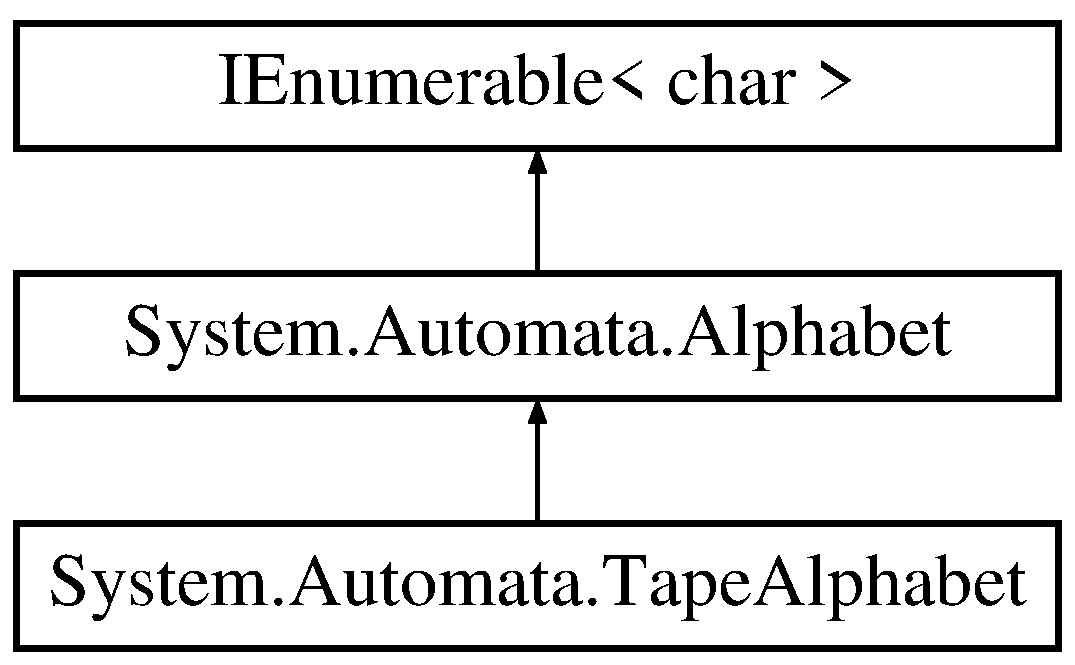
\includegraphics[height=3.000000cm]{class_system_1_1_automata_1_1_tape_alphabet}
\end{center}
\end{figure}
\subsection*{Public Member Functions}
\begin{DoxyCompactItemize}
\item 
\mbox{\Hypertarget{class_system_1_1_automata_1_1_tape_alphabet_ab22c5bbbc8ffa821c4e3dbfadb105b48}\label{class_system_1_1_automata_1_1_tape_alphabet_ab22c5bbbc8ffa821c4e3dbfadb105b48}} 
{\bfseries Tape\+Alphabet} (\mbox{\hyperlink{class_system_1_1_automata_1_1_alphabet}{Alphabet}} a, params char\mbox{[}$\,$\mbox{]} c)
\item 
\mbox{\Hypertarget{class_system_1_1_automata_1_1_tape_alphabet_a527ad315771a4fce4b3f5fd349d4ad6a}\label{class_system_1_1_automata_1_1_tape_alphabet_a527ad315771a4fce4b3f5fd349d4ad6a}} 
{\bfseries Tape\+Alphabet} (params char\mbox{[}$\,$\mbox{]} c)
\end{DoxyCompactItemize}
\subsection*{Static Public Member Functions}
\begin{DoxyCompactItemize}
\item 
\mbox{\Hypertarget{class_system_1_1_automata_1_1_tape_alphabet_ad161b4d2233c16e96c8d978fc7eee0be}\label{class_system_1_1_automata_1_1_tape_alphabet_ad161b4d2233c16e96c8d978fc7eee0be}} 
static \mbox{\hyperlink{class_system_1_1_automata_1_1_tape_alphabet}{Tape\+Alphabet}} {\bfseries operator+} (\mbox{\hyperlink{class_system_1_1_automata_1_1_tape_alphabet}{Tape\+Alphabet}} a, \mbox{\hyperlink{class_system_1_1_automata_1_1_alphabet}{Alphabet}} b)
\item 
\mbox{\Hypertarget{class_system_1_1_automata_1_1_tape_alphabet_a1f6473f626aad4c5bcaff854c82c2540}\label{class_system_1_1_automata_1_1_tape_alphabet_a1f6473f626aad4c5bcaff854c82c2540}} 
static \mbox{\hyperlink{class_system_1_1_automata_1_1_tape_alphabet}{Tape\+Alphabet}} {\bfseries operator+} (\mbox{\hyperlink{class_system_1_1_automata_1_1_alphabet}{Alphabet}} a, \mbox{\hyperlink{class_system_1_1_automata_1_1_tape_alphabet}{Tape\+Alphabet}} b)
\item 
\mbox{\Hypertarget{class_system_1_1_automata_1_1_tape_alphabet_a55a4b334be27c9236802ac1d3701d90a}\label{class_system_1_1_automata_1_1_tape_alphabet_a55a4b334be27c9236802ac1d3701d90a}} 
static \mbox{\hyperlink{class_system_1_1_automata_1_1_tape_alphabet}{Tape\+Alphabet}} {\bfseries operator+} (\mbox{\hyperlink{class_system_1_1_automata_1_1_tape_alphabet}{Tape\+Alphabet}} a, \mbox{\hyperlink{class_system_1_1_automata_1_1_tape_alphabet}{Tape\+Alphabet}} b)
\item 
\mbox{\Hypertarget{class_system_1_1_automata_1_1_tape_alphabet_a028150cbb9bf3f5bdbef1cd81b9df3fa}\label{class_system_1_1_automata_1_1_tape_alphabet_a028150cbb9bf3f5bdbef1cd81b9df3fa}} 
static \mbox{\hyperlink{class_system_1_1_automata_1_1_tape_alphabet}{Tape\+Alphabet}} {\bfseries operator-\/} (\mbox{\hyperlink{class_system_1_1_automata_1_1_tape_alphabet}{Tape\+Alphabet}} a, \mbox{\hyperlink{class_system_1_1_automata_1_1_alphabet}{Alphabet}} b)
\item 
\mbox{\Hypertarget{class_system_1_1_automata_1_1_tape_alphabet_a1b250cb143390b4a150ba32d9d5534e4}\label{class_system_1_1_automata_1_1_tape_alphabet_a1b250cb143390b4a150ba32d9d5534e4}} 
static \mbox{\hyperlink{class_system_1_1_automata_1_1_alphabet}{Alphabet}} {\bfseries operator-\/} (\mbox{\hyperlink{class_system_1_1_automata_1_1_alphabet}{Alphabet}} a, \mbox{\hyperlink{class_system_1_1_automata_1_1_tape_alphabet}{Tape\+Alphabet}} b)
\item 
\mbox{\Hypertarget{class_system_1_1_automata_1_1_tape_alphabet_a1126b4bcca9994dfbe34e0eaf79c9bc6}\label{class_system_1_1_automata_1_1_tape_alphabet_a1126b4bcca9994dfbe34e0eaf79c9bc6}} 
static \mbox{\hyperlink{class_system_1_1_automata_1_1_tape_alphabet}{Tape\+Alphabet}} {\bfseries operator-\/} (\mbox{\hyperlink{class_system_1_1_automata_1_1_tape_alphabet}{Tape\+Alphabet}} a, \mbox{\hyperlink{class_system_1_1_automata_1_1_tape_alphabet}{Tape\+Alphabet}} b)
\end{DoxyCompactItemize}
\subsection*{Additional Inherited Members}


\subsection{Detailed Description}
An alphabet for use with a Turing tape 



The documentation for this class was generated from the following file\+:\begin{DoxyCompactItemize}
\item 
System.\+Automata/Tape\+Alphabet.\+cs\end{DoxyCompactItemize}

\hypertarget{class_system_1_1_automata_1_1_transition}{}\section{System.\+Automata.\+Transition Class Reference}
\label{class_system_1_1_automata_1_1_transition}\index{System.\+Automata.\+Transition@{System.\+Automata.\+Transition}}


A state transition  


Inheritance diagram for System.\+Automata.\+Transition\+:\begin{figure}[H]
\begin{center}
\leavevmode
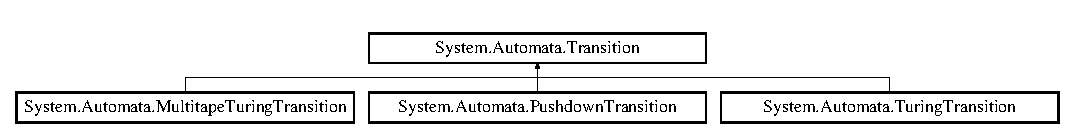
\includegraphics[height=1.424936cm]{class_system_1_1_automata_1_1_transition}
\end{center}
\end{figure}
\subsection*{Public Member Functions}
\begin{DoxyCompactItemize}
\item 
\mbox{\hyperlink{class_system_1_1_automata_1_1_transition_a15b9c85b9017f971a4d919975ed0d8d5}{Transition}} (\mbox{\hyperlink{class_system_1_1_automata_1_1_state}{State}} p, char c, \mbox{\hyperlink{class_system_1_1_automata_1_1_state}{State}} q)
\item 
\mbox{\Hypertarget{class_system_1_1_automata_1_1_transition_abdcef086901adb0c629d9c6507dc6697}\label{class_system_1_1_automata_1_1_transition_abdcef086901adb0c629d9c6507dc6697}} 
override string {\bfseries To\+String} ()
\end{DoxyCompactItemize}
\subsection*{Properties}
\begin{DoxyCompactItemize}
\item 
\mbox{\hyperlink{class_system_1_1_automata_1_1_state}{State}} \mbox{\hyperlink{class_system_1_1_automata_1_1_transition_adbb06230aadfde954396097f721ba575}{P}}\hspace{0.3cm}{\ttfamily  \mbox{[}get\mbox{]}}
\begin{DoxyCompactList}\small\item\em The current state. \end{DoxyCompactList}\item 
\mbox{\hyperlink{class_system_1_1_automata_1_1_state}{State}} \mbox{\hyperlink{class_system_1_1_automata_1_1_transition_a41e49dbbe374855b54fe12112c317dc4}{Q}}\hspace{0.3cm}{\ttfamily  \mbox{[}get\mbox{]}}
\begin{DoxyCompactList}\small\item\em The next state. \end{DoxyCompactList}\item 
char \mbox{\hyperlink{class_system_1_1_automata_1_1_transition_a692777c086d9aab84c1c3cce3a769473}{A}}\hspace{0.3cm}{\ttfamily  \mbox{[}get\mbox{]}}
\begin{DoxyCompactList}\small\item\em The symbol to transition on \end{DoxyCompactList}\end{DoxyCompactItemize}


\subsection{Detailed Description}
A state transition 



\subsection{Constructor \& Destructor Documentation}
\mbox{\Hypertarget{class_system_1_1_automata_1_1_transition_a15b9c85b9017f971a4d919975ed0d8d5}\label{class_system_1_1_automata_1_1_transition_a15b9c85b9017f971a4d919975ed0d8d5}} 
\index{System\+::\+Automata\+::\+Transition@{System\+::\+Automata\+::\+Transition}!Transition@{Transition}}
\index{Transition@{Transition}!System\+::\+Automata\+::\+Transition@{System\+::\+Automata\+::\+Transition}}
\subsubsection{\texorpdfstring{Transition()}{Transition()}}
{\footnotesize\ttfamily System.\+Automata.\+Transition.\+Transition (\begin{DoxyParamCaption}\item[{\mbox{\hyperlink{class_system_1_1_automata_1_1_state}{State}}}]{p,  }\item[{char}]{c,  }\item[{\mbox{\hyperlink{class_system_1_1_automata_1_1_state}{State}}}]{q }\end{DoxyParamCaption})}


\begin{DoxyParams}{Parameters}
{\em p} & The current state\\
\hline
{\em c} & The current input symbol\\
\hline
{\em q} & The next state\\
\hline
\end{DoxyParams}


For a epsilon-\/transition, use \mbox{\hyperlink{class_system_1_1_automata_1_1_alphabet}{Alphabet}}.\mbox{\hyperlink{class_system_1_1_automata_1_1_alphabet_aa3f8c16de4596ed24f2fe0fb77e7493c}{Alphabet.\+Empty\+String}}

\subsection{Property Documentation}
\mbox{\Hypertarget{class_system_1_1_automata_1_1_transition_a692777c086d9aab84c1c3cce3a769473}\label{class_system_1_1_automata_1_1_transition_a692777c086d9aab84c1c3cce3a769473}} 
\index{System\+::\+Automata\+::\+Transition@{System\+::\+Automata\+::\+Transition}!A@{A}}
\index{A@{A}!System\+::\+Automata\+::\+Transition@{System\+::\+Automata\+::\+Transition}}
\subsubsection{\texorpdfstring{A}{A}}
{\footnotesize\ttfamily char System.\+Automata.\+Transition.\+A\hspace{0.3cm}{\ttfamily [get]}}



The symbol to transition on 

\mbox{\Hypertarget{class_system_1_1_automata_1_1_transition_adbb06230aadfde954396097f721ba575}\label{class_system_1_1_automata_1_1_transition_adbb06230aadfde954396097f721ba575}} 
\index{System\+::\+Automata\+::\+Transition@{System\+::\+Automata\+::\+Transition}!P@{P}}
\index{P@{P}!System\+::\+Automata\+::\+Transition@{System\+::\+Automata\+::\+Transition}}
\subsubsection{\texorpdfstring{P}{P}}
{\footnotesize\ttfamily \mbox{\hyperlink{class_system_1_1_automata_1_1_state}{State}} System.\+Automata.\+Transition.\+P\hspace{0.3cm}{\ttfamily [get]}}



The current state. 

\mbox{\Hypertarget{class_system_1_1_automata_1_1_transition_a41e49dbbe374855b54fe12112c317dc4}\label{class_system_1_1_automata_1_1_transition_a41e49dbbe374855b54fe12112c317dc4}} 
\index{System\+::\+Automata\+::\+Transition@{System\+::\+Automata\+::\+Transition}!Q@{Q}}
\index{Q@{Q}!System\+::\+Automata\+::\+Transition@{System\+::\+Automata\+::\+Transition}}
\subsubsection{\texorpdfstring{Q}{Q}}
{\footnotesize\ttfamily \mbox{\hyperlink{class_system_1_1_automata_1_1_state}{State}} System.\+Automata.\+Transition.\+Q\hspace{0.3cm}{\ttfamily [get]}}



The next state. 



The documentation for this class was generated from the following file\+:\begin{DoxyCompactItemize}
\item 
System.\+Automata/Transition.\+cs\end{DoxyCompactItemize}

\hypertarget{class_system_1_1_automata_1_1_transition_function}{}\section{System.\+Automata.\+Transition\+Function Class Reference}
\label{class_system_1_1_automata_1_1_transition_function}\index{System.\+Automata.\+Transition\+Function@{System.\+Automata.\+Transition\+Function}}


A deterministic collection of state transition mappings.  


Inheritance diagram for System.\+Automata.\+Transition\+Function\+:\begin{figure}[H]
\begin{center}
\leavevmode
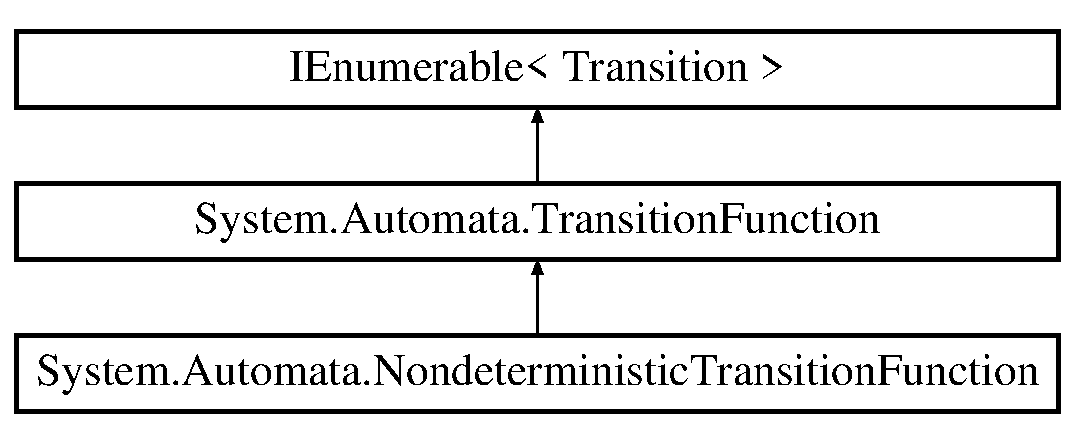
\includegraphics[height=3.000000cm]{class_system_1_1_automata_1_1_transition_function}
\end{center}
\end{figure}
\subsection*{Public Member Functions}
\begin{DoxyCompactItemize}
\item 
\mbox{\Hypertarget{class_system_1_1_automata_1_1_transition_function_a2eb826c0a54140e72ccd5e7f092ec7a4}\label{class_system_1_1_automata_1_1_transition_function_a2eb826c0a54140e72ccd5e7f092ec7a4}} 
{\bfseries Transition\+Function} (params \mbox{\hyperlink{class_system_1_1_automata_1_1_transition}{Transition}}\mbox{[}$\,$\mbox{]} t)
\item 
void \mbox{\hyperlink{class_system_1_1_automata_1_1_transition_function_a14ad89fa854a2d313381f986d348be88}{Add}} (\mbox{\hyperlink{class_system_1_1_automata_1_1_transition}{Transition}} t)
\begin{DoxyCompactList}\small\item\em Add a transition to the function \end{DoxyCompactList}\item 
\mbox{\Hypertarget{class_system_1_1_automata_1_1_transition_function_a73aeeac22367c08bf2dac0068c726a60}\label{class_system_1_1_automata_1_1_transition_function_a73aeeac22367c08bf2dac0068c726a60}} 
bool {\bfseries Contains} (\mbox{\hyperlink{class_system_1_1_automata_1_1_transition}{Transition}} t)
\item 
\mbox{\Hypertarget{class_system_1_1_automata_1_1_transition_function_a397318c941b1f3b0b349c945f7b71109}\label{class_system_1_1_automata_1_1_transition_function_a397318c941b1f3b0b349c945f7b71109}} 
bool {\bfseries Exists} (Predicate$<$ \mbox{\hyperlink{class_system_1_1_automata_1_1_transition}{Transition}} $>$ p)
\item 
\mbox{\Hypertarget{class_system_1_1_automata_1_1_transition_function_a5ef277ec52104ed77a05056dc6fa1895}\label{class_system_1_1_automata_1_1_transition_function_a5ef277ec52104ed77a05056dc6fa1895}} 
I\+Enumerator$<$ \mbox{\hyperlink{class_system_1_1_automata_1_1_transition}{Transition}} $>$ {\bfseries Get\+Enumerator} ()
\end{DoxyCompactItemize}
\subsection*{Public Attributes}
\begin{DoxyCompactItemize}
\item 
\mbox{\Hypertarget{class_system_1_1_automata_1_1_transition_function_abcc64a0e83783e95e29985d157d74f6b}\label{class_system_1_1_automata_1_1_transition_function_abcc64a0e83783e95e29985d157d74f6b}} 
int {\bfseries Count} =$>$ Trans.\+Count
\item 
\mbox{\hyperlink{class_system_1_1_automata_1_1_transition}{Transition}} \mbox{\hyperlink{class_system_1_1_automata_1_1_transition_function_a887174305e7741235859aceff5556bbd}{this\mbox{[}\+State p, char s\mbox{]}}} =$>$ Get(p, s)
\begin{DoxyCompactList}\small\item\em Get the next state \mbox{\hyperlink{class_system_1_1_automata_1_1_transition}{Transition}} \end{DoxyCompactList}\end{DoxyCompactItemize}
\subsection*{Protected Attributes}
\begin{DoxyCompactItemize}
\item 
\mbox{\Hypertarget{class_system_1_1_automata_1_1_transition_function_a565d701a23b82c6546ce8d5c8fbc7862}\label{class_system_1_1_automata_1_1_transition_function_a565d701a23b82c6546ce8d5c8fbc7862}} 
List$<$ \mbox{\hyperlink{class_system_1_1_automata_1_1_transition}{Transition}} $>$ {\bfseries Trans}
\end{DoxyCompactItemize}


\subsection{Detailed Description}
A deterministic collection of state transition mappings. 



\subsection{Member Function Documentation}
\mbox{\Hypertarget{class_system_1_1_automata_1_1_transition_function_a14ad89fa854a2d313381f986d348be88}\label{class_system_1_1_automata_1_1_transition_function_a14ad89fa854a2d313381f986d348be88}} 
\index{System\+::\+Automata\+::\+Transition\+Function@{System\+::\+Automata\+::\+Transition\+Function}!Add@{Add}}
\index{Add@{Add}!System\+::\+Automata\+::\+Transition\+Function@{System\+::\+Automata\+::\+Transition\+Function}}
\subsubsection{\texorpdfstring{Add()}{Add()}}
{\footnotesize\ttfamily void System.\+Automata.\+Transition\+Function.\+Add (\begin{DoxyParamCaption}\item[{\mbox{\hyperlink{class_system_1_1_automata_1_1_transition}{Transition}}}]{t }\end{DoxyParamCaption})}



Add a transition to the function 


\begin{DoxyParams}{Parameters}
{\em t} & The transition to add\\
\hline
\end{DoxyParams}

\begin{DoxyExceptions}{Exceptions}
{\em Null\+Reference\+Exception} & If a transition has a null state\\
\hline
{\em Argument\+Exception} & If a null transition (using Empty\+String) was added\\
\hline
\end{DoxyExceptions}


Not thread safe! Do not use after adding the function to an automaton.

\subsection{Member Data Documentation}
\mbox{\Hypertarget{class_system_1_1_automata_1_1_transition_function_a887174305e7741235859aceff5556bbd}\label{class_system_1_1_automata_1_1_transition_function_a887174305e7741235859aceff5556bbd}} 
\index{System\+::\+Automata\+::\+Transition\+Function@{System\+::\+Automata\+::\+Transition\+Function}!this\mbox{[}\+State p, char s\mbox{]}@{this[State p, char s]}}
\index{this\mbox{[}\+State p, char s\mbox{]}@{this[State p, char s]}!System\+::\+Automata\+::\+Transition\+Function@{System\+::\+Automata\+::\+Transition\+Function}}
\subsubsection{\texorpdfstring{this[State p, char s]}{this[State p, char s]}}
{\footnotesize\ttfamily \mbox{\hyperlink{class_system_1_1_automata_1_1_transition}{Transition}} System.\+Automata.\+Transition\+Function.\+this\mbox{[}\mbox{\hyperlink{class_system_1_1_automata_1_1_state}{State}} p, char s\mbox{]} =$>$ Get(p, s)}



Get the next state \mbox{\hyperlink{class_system_1_1_automata_1_1_transition}{Transition}} 


\begin{DoxyParams}{Parameters}
{\em p} & The current state\\
\hline
{\em s} & The current input character\\
\hline
\end{DoxyParams}


The documentation for this class was generated from the following file\+:\begin{DoxyCompactItemize}
\item 
System.\+Automata/Transition\+Function.\+cs\end{DoxyCompactItemize}

\hypertarget{class_system_1_1_automata_1_1_turing_machine}{}\section{System.\+Automata.\+Turing\+Machine Class Reference}
\label{class_system_1_1_automata_1_1_turing_machine}\index{System.\+Automata.\+Turing\+Machine@{System.\+Automata.\+Turing\+Machine}}


A nondeterministic Turing machine  


Inheritance diagram for System.\+Automata.\+Turing\+Machine\+:\begin{figure}[H]
\begin{center}
\leavevmode
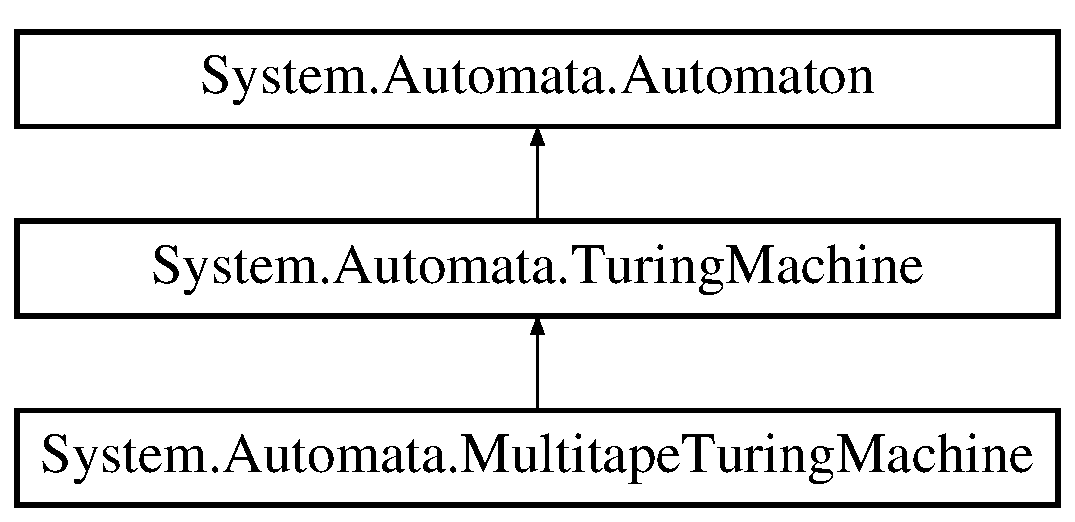
\includegraphics[height=3.000000cm]{class_system_1_1_automata_1_1_turing_machine}
\end{center}
\end{figure}
\subsection*{Public Types}
\begin{DoxyCompactItemize}
\item 
enum \mbox{\hyperlink{class_system_1_1_automata_1_1_turing_machine_aa253c3820befa3cfdd3d17b2d8fdd2d9}{Direction}} \{ \mbox{\hyperlink{class_system_1_1_automata_1_1_turing_machine_aa253c3820befa3cfdd3d17b2d8fdd2d9ad20caec3b48a1eef164cb4ca81ba2587}{Direction.\+L}}, 
\mbox{\hyperlink{class_system_1_1_automata_1_1_turing_machine_aa253c3820befa3cfdd3d17b2d8fdd2d9ae1e1d3d40573127e9ee0480caf1283d6}{Direction.\+R}}, 
\mbox{\hyperlink{class_system_1_1_automata_1_1_turing_machine_aa253c3820befa3cfdd3d17b2d8fdd2d9a5dbc98dcc983a70728bd082d1a47546e}{Direction.\+S}}
 \}
\begin{DoxyCompactList}\small\item\em The direction to move the tape \end{DoxyCompactList}\end{DoxyCompactItemize}
\subsection*{Public Member Functions}
\begin{DoxyCompactItemize}
\item 
\mbox{\Hypertarget{class_system_1_1_automata_1_1_turing_machine_aaa0a99528675b0d136a68f9e0981d3fa}\label{class_system_1_1_automata_1_1_turing_machine_aaa0a99528675b0d136a68f9e0981d3fa}} 
{\bfseries Turing\+Machine} (\mbox{\hyperlink{class_system_1_1_automata_1_1_states}{States}} q, \mbox{\hyperlink{class_system_1_1_automata_1_1_alphabet}{Alphabet}} a, \mbox{\hyperlink{class_system_1_1_automata_1_1_tape_alphabet}{Tape\+Alphabet}} g, \mbox{\hyperlink{class_system_1_1_automata_1_1_turing_transition_function}{Turing\+Transition\+Function}} tf, \mbox{\hyperlink{class_system_1_1_automata_1_1_state}{State}} q0)
\item 
bool \mbox{\hyperlink{class_system_1_1_automata_1_1_turing_machine_a49d164f2e9784ad4ac23410c702ad1b0}{Run}} (I\+Enumerable$<$ char $>$ x, out char\mbox{[}$\,$\mbox{]} o)
\begin{DoxyCompactList}\small\item\em Run the machine \end{DoxyCompactList}\item 
\mbox{\Hypertarget{class_system_1_1_automata_1_1_turing_machine_a4392d8174f54fb36a8c4ef86161ef6c8}\label{class_system_1_1_automata_1_1_turing_machine_a4392d8174f54fb36a8c4ef86161ef6c8}} 
bool {\bfseries Run} (I\+Enumerable$<$ char $>$ x)
\item 
\mbox{\Hypertarget{class_system_1_1_automata_1_1_turing_machine_a98e84b8b1e0e551cb07ff9408606196c}\label{class_system_1_1_automata_1_1_turing_machine_a98e84b8b1e0e551cb07ff9408606196c}} 
bool {\bfseries Run} (string x, out char\mbox{[}$\,$\mbox{]} o)
\item 
\mbox{\Hypertarget{class_system_1_1_automata_1_1_turing_machine_a765c176211ed3dd0381728b1c90ba36c}\label{class_system_1_1_automata_1_1_turing_machine_a765c176211ed3dd0381728b1c90ba36c}} 
bool {\bfseries Run} (string x)
\end{DoxyCompactItemize}
\subsection*{Static Public Member Functions}
\begin{DoxyCompactItemize}
\item 
static string \mbox{\hyperlink{class_system_1_1_automata_1_1_turing_machine_a91f5ff324232a1377aa280bc7649acb5}{Bin\+Encode}} (int x)
\item 
static string \mbox{\hyperlink{class_system_1_1_automata_1_1_turing_machine_a256b8d185c89a85dc7c27b02e8f61684}{Bin\+Encode}} (char x)
\item 
static string \mbox{\hyperlink{class_system_1_1_automata_1_1_turing_machine_a9f6c774477e3ed6600244bb0ffbe1579}{Bin\+Encode}} (char\mbox{[}$\,$\mbox{]} x)
\item 
static string \mbox{\hyperlink{class_system_1_1_automata_1_1_turing_machine_a559b0d5709eab0bd072c9ae1da449cf4}{Bin\+Encode}} (string x)
\item 
static string \mbox{\hyperlink{class_system_1_1_automata_1_1_turing_machine_ad62c28bec4c48435a98b4eb5edb89487}{Unary\+Encode}} (uint n)
\item 
static string \mbox{\hyperlink{class_system_1_1_automata_1_1_turing_machine_a46274b3df870b1f350b8067e4eda77d9}{Bin\+Encode}} (\mbox{\hyperlink{class_system_1_1_automata_1_1_turing_machine}{Turing\+Machine}} t, char\mbox{[}$\,$\mbox{]} x=null)
\begin{DoxyCompactList}\small\item\em Encode a turing machine \end{DoxyCompactList}\item 
static string \mbox{\hyperlink{class_system_1_1_automata_1_1_turing_machine_ae14f5c2439f706832f06cfc712e27b93}{Bin\+Encode}} (\mbox{\hyperlink{class_system_1_1_automata_1_1_turing_transition}{Turing\+Transition}} t, \mbox{\hyperlink{class_system_1_1_automata_1_1_states}{States}} s)
\begin{DoxyCompactList}\small\item\em Encode a turing machine move \end{DoxyCompactList}\end{DoxyCompactItemize}
\subsection*{Static Public Attributes}
\begin{DoxyCompactItemize}
\item 
\mbox{\Hypertarget{class_system_1_1_automata_1_1_turing_machine_a95b030005a20801b27d0ec17aa017766}\label{class_system_1_1_automata_1_1_turing_machine_a95b030005a20801b27d0ec17aa017766}} 
static new readonly \mbox{\hyperlink{class_system_1_1_automata_1_1_accepting_states}{Accepting\+States}} {\bfseries Accepting\+States} = new \mbox{\hyperlink{class_system_1_1_automata_1_1_accepting_states}{Accepting\+States}}(\mbox{\hyperlink{class_system_1_1_automata_1_1_state_ae6639cebabe973cfa8825fedbc4ae741}{State.\+Ha}})
\end{DoxyCompactItemize}
\subsection*{Protected Member Functions}
\begin{DoxyCompactItemize}
\item 
\mbox{\Hypertarget{class_system_1_1_automata_1_1_turing_machine_ad58e324621c3250dc8b5158c8ead621f}\label{class_system_1_1_automata_1_1_turing_machine_ad58e324621c3250dc8b5158c8ead621f}} 
int {\bfseries Move\+Tape\+Head} (int i, \mbox{\hyperlink{class_system_1_1_automata_1_1_turing_machine_aa253c3820befa3cfdd3d17b2d8fdd2d9}{Direction}} d)
\end{DoxyCompactItemize}
\subsection*{Properties}
\begin{DoxyCompactItemize}
\item 
\mbox{\hyperlink{class_system_1_1_automata_1_1_tape_alphabet}{Tape\+Alphabet}} \mbox{\hyperlink{class_system_1_1_automata_1_1_turing_machine_a6f92addf3d029757073431b5b4758cdb}{Tape\+Alphabet}}\hspace{0.3cm}{\ttfamily  \mbox{[}get, protected set\mbox{]}}
\begin{DoxyCompactList}\small\item\em The tape alphabet. \end{DoxyCompactList}\item 
\mbox{\Hypertarget{class_system_1_1_automata_1_1_turing_machine_a7852b38b2d6a3f734ff2075bb2c3831b}\label{class_system_1_1_automata_1_1_turing_machine_a7852b38b2d6a3f734ff2075bb2c3831b}} 
new \mbox{\hyperlink{class_system_1_1_automata_1_1_turing_transition_function}{Turing\+Transition\+Function}} {\bfseries Transitions}\hspace{0.3cm}{\ttfamily  \mbox{[}get\mbox{]}}
\end{DoxyCompactItemize}


\subsection{Detailed Description}
A nondeterministic Turing machine 



\subsection{Member Enumeration Documentation}
\mbox{\Hypertarget{class_system_1_1_automata_1_1_turing_machine_aa253c3820befa3cfdd3d17b2d8fdd2d9}\label{class_system_1_1_automata_1_1_turing_machine_aa253c3820befa3cfdd3d17b2d8fdd2d9}} 
\index{System\+::\+Automata\+::\+Turing\+Machine@{System\+::\+Automata\+::\+Turing\+Machine}!Direction@{Direction}}
\index{Direction@{Direction}!System\+::\+Automata\+::\+Turing\+Machine@{System\+::\+Automata\+::\+Turing\+Machine}}
\subsubsection{\texorpdfstring{Direction}{Direction}}
{\footnotesize\ttfamily enum \mbox{\hyperlink{class_system_1_1_automata_1_1_turing_machine_aa253c3820befa3cfdd3d17b2d8fdd2d9}{System.\+Automata.\+Turing\+Machine.\+Direction}}\hspace{0.3cm}{\ttfamily [strong]}}



The direction to move the tape 

\begin{DoxyEnumFields}{Enumerator}
\raisebox{\heightof{T}}[0pt][0pt]{\index{L@{L}!System\+::\+Automata\+::\+Turing\+Machine@{System\+::\+Automata\+::\+Turing\+Machine}}\index{System\+::\+Automata\+::\+Turing\+Machine@{System\+::\+Automata\+::\+Turing\+Machine}!L@{L}}}\mbox{\Hypertarget{class_system_1_1_automata_1_1_turing_machine_aa253c3820befa3cfdd3d17b2d8fdd2d9ad20caec3b48a1eef164cb4ca81ba2587}\label{class_system_1_1_automata_1_1_turing_machine_aa253c3820befa3cfdd3d17b2d8fdd2d9ad20caec3b48a1eef164cb4ca81ba2587}} 
L&Move the tape head left one cell. \\
\hline

\raisebox{\heightof{T}}[0pt][0pt]{\index{R@{R}!System\+::\+Automata\+::\+Turing\+Machine@{System\+::\+Automata\+::\+Turing\+Machine}}\index{System\+::\+Automata\+::\+Turing\+Machine@{System\+::\+Automata\+::\+Turing\+Machine}!R@{R}}}\mbox{\Hypertarget{class_system_1_1_automata_1_1_turing_machine_aa253c3820befa3cfdd3d17b2d8fdd2d9ae1e1d3d40573127e9ee0480caf1283d6}\label{class_system_1_1_automata_1_1_turing_machine_aa253c3820befa3cfdd3d17b2d8fdd2d9ae1e1d3d40573127e9ee0480caf1283d6}} 
R&Move the tape head right one cell. \\
\hline

\raisebox{\heightof{T}}[0pt][0pt]{\index{S@{S}!System\+::\+Automata\+::\+Turing\+Machine@{System\+::\+Automata\+::\+Turing\+Machine}}\index{System\+::\+Automata\+::\+Turing\+Machine@{System\+::\+Automata\+::\+Turing\+Machine}!S@{S}}}\mbox{\Hypertarget{class_system_1_1_automata_1_1_turing_machine_aa253c3820befa3cfdd3d17b2d8fdd2d9a5dbc98dcc983a70728bd082d1a47546e}\label{class_system_1_1_automata_1_1_turing_machine_aa253c3820befa3cfdd3d17b2d8fdd2d9a5dbc98dcc983a70728bd082d1a47546e}} 
S&Do not move the tape head. \\
\hline

\end{DoxyEnumFields}


\subsection{Member Function Documentation}
\mbox{\Hypertarget{class_system_1_1_automata_1_1_turing_machine_a91f5ff324232a1377aa280bc7649acb5}\label{class_system_1_1_automata_1_1_turing_machine_a91f5ff324232a1377aa280bc7649acb5}} 
\index{System\+::\+Automata\+::\+Turing\+Machine@{System\+::\+Automata\+::\+Turing\+Machine}!Bin\+Encode@{Bin\+Encode}}
\index{Bin\+Encode@{Bin\+Encode}!System\+::\+Automata\+::\+Turing\+Machine@{System\+::\+Automata\+::\+Turing\+Machine}}
\subsubsection{\texorpdfstring{Bin\+Encode()}{BinEncode()}\hspace{0.1cm}{\footnotesize\ttfamily [1/6]}}
{\footnotesize\ttfamily static string System.\+Automata.\+Turing\+Machine.\+Bin\+Encode (\begin{DoxyParamCaption}\item[{int}]{x }\end{DoxyParamCaption})\hspace{0.3cm}{\ttfamily [static]}}


\begin{DoxyParams}{Parameters}
{\em x} & The number to encode\\
\hline
\end{DoxyParams}
\begin{DoxyReturn}{Returns}
The integer as a binary number
\end{DoxyReturn}


32-\/bits with two\textquotesingle{}s complement for negatives, without leading 0s\mbox{\Hypertarget{class_system_1_1_automata_1_1_turing_machine_a256b8d185c89a85dc7c27b02e8f61684}\label{class_system_1_1_automata_1_1_turing_machine_a256b8d185c89a85dc7c27b02e8f61684}} 
\index{System\+::\+Automata\+::\+Turing\+Machine@{System\+::\+Automata\+::\+Turing\+Machine}!Bin\+Encode@{Bin\+Encode}}
\index{Bin\+Encode@{Bin\+Encode}!System\+::\+Automata\+::\+Turing\+Machine@{System\+::\+Automata\+::\+Turing\+Machine}}
\subsubsection{\texorpdfstring{Bin\+Encode()}{BinEncode()}\hspace{0.1cm}{\footnotesize\ttfamily [2/6]}}
{\footnotesize\ttfamily static string System.\+Automata.\+Turing\+Machine.\+Bin\+Encode (\begin{DoxyParamCaption}\item[{char}]{x }\end{DoxyParamCaption})\hspace{0.3cm}{\ttfamily [static]}}


\begin{DoxyParams}{Parameters}
{\em x} & The character to encode\\
\hline
\end{DoxyParams}
\begin{DoxyReturn}{Returns}
The character as an A\+S\+C\+II binary number without leading 0s
\end{DoxyReturn}
\mbox{\Hypertarget{class_system_1_1_automata_1_1_turing_machine_a9f6c774477e3ed6600244bb0ffbe1579}\label{class_system_1_1_automata_1_1_turing_machine_a9f6c774477e3ed6600244bb0ffbe1579}} 
\index{System\+::\+Automata\+::\+Turing\+Machine@{System\+::\+Automata\+::\+Turing\+Machine}!Bin\+Encode@{Bin\+Encode}}
\index{Bin\+Encode@{Bin\+Encode}!System\+::\+Automata\+::\+Turing\+Machine@{System\+::\+Automata\+::\+Turing\+Machine}}
\subsubsection{\texorpdfstring{Bin\+Encode()}{BinEncode()}\hspace{0.1cm}{\footnotesize\ttfamily [3/6]}}
{\footnotesize\ttfamily static string System.\+Automata.\+Turing\+Machine.\+Bin\+Encode (\begin{DoxyParamCaption}\item[{char \mbox{[}$\,$\mbox{]}}]{x }\end{DoxyParamCaption})\hspace{0.3cm}{\ttfamily [static]}}


\begin{DoxyParams}{Parameters}
{\em x} & The string to encode\\
\hline
\end{DoxyParams}
\begin{DoxyReturn}{Returns}
A string of the form e(x0)Δe(x1)Δ..Δe(xk)Δ where e(xk) is the binary encoding of a single character.
\end{DoxyReturn}
\mbox{\Hypertarget{class_system_1_1_automata_1_1_turing_machine_a559b0d5709eab0bd072c9ae1da449cf4}\label{class_system_1_1_automata_1_1_turing_machine_a559b0d5709eab0bd072c9ae1da449cf4}} 
\index{System\+::\+Automata\+::\+Turing\+Machine@{System\+::\+Automata\+::\+Turing\+Machine}!Bin\+Encode@{Bin\+Encode}}
\index{Bin\+Encode@{Bin\+Encode}!System\+::\+Automata\+::\+Turing\+Machine@{System\+::\+Automata\+::\+Turing\+Machine}}
\subsubsection{\texorpdfstring{Bin\+Encode()}{BinEncode()}\hspace{0.1cm}{\footnotesize\ttfamily [4/6]}}
{\footnotesize\ttfamily static string System.\+Automata.\+Turing\+Machine.\+Bin\+Encode (\begin{DoxyParamCaption}\item[{string}]{x }\end{DoxyParamCaption})\hspace{0.3cm}{\ttfamily [static]}}


\begin{DoxyParams}{Parameters}
{\em x} & The string to encode\\
\hline
\end{DoxyParams}
\begin{DoxyReturn}{Returns}
A string of the form e(x0)Δe(x1)Δ..Δe(xk)Δ where e(xk) is the binary encoding of a single character.
\end{DoxyReturn}
\mbox{\Hypertarget{class_system_1_1_automata_1_1_turing_machine_a46274b3df870b1f350b8067e4eda77d9}\label{class_system_1_1_automata_1_1_turing_machine_a46274b3df870b1f350b8067e4eda77d9}} 
\index{System\+::\+Automata\+::\+Turing\+Machine@{System\+::\+Automata\+::\+Turing\+Machine}!Bin\+Encode@{Bin\+Encode}}
\index{Bin\+Encode@{Bin\+Encode}!System\+::\+Automata\+::\+Turing\+Machine@{System\+::\+Automata\+::\+Turing\+Machine}}
\subsubsection{\texorpdfstring{Bin\+Encode()}{BinEncode()}\hspace{0.1cm}{\footnotesize\ttfamily [5/6]}}
{\footnotesize\ttfamily static string System.\+Automata.\+Turing\+Machine.\+Bin\+Encode (\begin{DoxyParamCaption}\item[{\mbox{\hyperlink{class_system_1_1_automata_1_1_turing_machine}{Turing\+Machine}}}]{t,  }\item[{char \mbox{[}$\,$\mbox{]}}]{x = {\ttfamily null} }\end{DoxyParamCaption})\hspace{0.3cm}{\ttfamily [static]}}



Encode a turing machine 


\begin{DoxyParams}{Parameters}
{\em t} & The turing machine to encode\\
\hline
{\em x} & The input to encode\\
\hline
\end{DoxyParams}
\begin{DoxyReturn}{Returns}
A string ∈ \{0, 1, Δ\}$\ast$ representing a turing machine in the form Δe(m0)Δe(m1)Δ..Δe(mk)Δe(x) Where mk is a transition and e is the binary encoding function. 
\end{DoxyReturn}


See Bin\+Encode(\+Turing\+Transition) and Bin\+Encode(char\mbox{[}$\,$\mbox{]}) for specific encodings.\mbox{\Hypertarget{class_system_1_1_automata_1_1_turing_machine_ae14f5c2439f706832f06cfc712e27b93}\label{class_system_1_1_automata_1_1_turing_machine_ae14f5c2439f706832f06cfc712e27b93}} 
\index{System\+::\+Automata\+::\+Turing\+Machine@{System\+::\+Automata\+::\+Turing\+Machine}!Bin\+Encode@{Bin\+Encode}}
\index{Bin\+Encode@{Bin\+Encode}!System\+::\+Automata\+::\+Turing\+Machine@{System\+::\+Automata\+::\+Turing\+Machine}}
\subsubsection{\texorpdfstring{Bin\+Encode()}{BinEncode()}\hspace{0.1cm}{\footnotesize\ttfamily [6/6]}}
{\footnotesize\ttfamily static string System.\+Automata.\+Turing\+Machine.\+Bin\+Encode (\begin{DoxyParamCaption}\item[{\mbox{\hyperlink{class_system_1_1_automata_1_1_turing_transition}{Turing\+Transition}}}]{t,  }\item[{\mbox{\hyperlink{class_system_1_1_automata_1_1_states}{States}}}]{s }\end{DoxyParamCaption})\hspace{0.3cm}{\ttfamily [static]}}



Encode a turing machine move 


\begin{DoxyParams}{Parameters}
{\em t} & The transition\\
\hline
{\em s} & The set of states\\
\hline
\end{DoxyParams}
\begin{DoxyReturn}{Returns}
A string ∈ \{0, 1, Δ\}$\ast$ representing a turing transition 𝛿(p, σ) = (q, τ, D) where p,q ∈ S, σ,τ ∈ Σ in the form n(indexof(p))Δn(σ)Δn(indexof(q))Δn(τ)Δn(\+D)Δ where n(x) reperesents the binary integer or U\+TF representation of x. n(\+D) = \{ L-\/$>$00, R-\/$>$01, S-\/$>$10, err-\/$>$11 \} 
\end{DoxyReturn}

\begin{DoxyExceptions}{Exceptions}
{\em Argument\+Exception} & If a state referenced is not contained in s\\
\hline
\end{DoxyExceptions}
\mbox{\Hypertarget{class_system_1_1_automata_1_1_turing_machine_a49d164f2e9784ad4ac23410c702ad1b0}\label{class_system_1_1_automata_1_1_turing_machine_a49d164f2e9784ad4ac23410c702ad1b0}} 
\index{System\+::\+Automata\+::\+Turing\+Machine@{System\+::\+Automata\+::\+Turing\+Machine}!Run@{Run}}
\index{Run@{Run}!System\+::\+Automata\+::\+Turing\+Machine@{System\+::\+Automata\+::\+Turing\+Machine}}
\subsubsection{\texorpdfstring{Run()}{Run()}}
{\footnotesize\ttfamily bool System.\+Automata.\+Turing\+Machine.\+Run (\begin{DoxyParamCaption}\item[{I\+Enumerable$<$ char $>$}]{x,  }\item[{out char \mbox{[}$\,$\mbox{]}}]{o }\end{DoxyParamCaption})}



Run the machine 


\begin{DoxyParams}{Parameters}
{\em x} & The input to run the machine on.\\
\hline
{\em o} & The completed tape contents\\
\hline
\end{DoxyParams}
\begin{DoxyReturn}{Returns}
True if the machine halts in the accept state.
\end{DoxyReturn}


The first move the machine makes is to fill the tape with the blank symbol followed by the input.\mbox{\Hypertarget{class_system_1_1_automata_1_1_turing_machine_ad62c28bec4c48435a98b4eb5edb89487}\label{class_system_1_1_automata_1_1_turing_machine_ad62c28bec4c48435a98b4eb5edb89487}} 
\index{System\+::\+Automata\+::\+Turing\+Machine@{System\+::\+Automata\+::\+Turing\+Machine}!Unary\+Encode@{Unary\+Encode}}
\index{Unary\+Encode@{Unary\+Encode}!System\+::\+Automata\+::\+Turing\+Machine@{System\+::\+Automata\+::\+Turing\+Machine}}
\subsubsection{\texorpdfstring{Unary\+Encode()}{UnaryEncode()}}
{\footnotesize\ttfamily static string System.\+Automata.\+Turing\+Machine.\+Unary\+Encode (\begin{DoxyParamCaption}\item[{uint}]{n }\end{DoxyParamCaption})\hspace{0.3cm}{\ttfamily [static]}}


\begin{DoxyParams}{Parameters}
{\em n} & The number to encode\\
\hline
\end{DoxyParams}
\begin{DoxyReturn}{Returns}
The number n returned as the string 1$^\wedge$n
\end{DoxyReturn}


\subsection{Property Documentation}
\mbox{\Hypertarget{class_system_1_1_automata_1_1_turing_machine_a6f92addf3d029757073431b5b4758cdb}\label{class_system_1_1_automata_1_1_turing_machine_a6f92addf3d029757073431b5b4758cdb}} 
\index{System\+::\+Automata\+::\+Turing\+Machine@{System\+::\+Automata\+::\+Turing\+Machine}!Tape\+Alphabet@{Tape\+Alphabet}}
\index{Tape\+Alphabet@{Tape\+Alphabet}!System\+::\+Automata\+::\+Turing\+Machine@{System\+::\+Automata\+::\+Turing\+Machine}}
\subsubsection{\texorpdfstring{Tape\+Alphabet}{TapeAlphabet}}
{\footnotesize\ttfamily \mbox{\hyperlink{class_system_1_1_automata_1_1_tape_alphabet}{Tape\+Alphabet}} System.\+Automata.\+Turing\+Machine.\+Tape\+Alphabet\hspace{0.3cm}{\ttfamily [get]}, {\ttfamily [protected set]}}



The tape alphabet. 



The documentation for this class was generated from the following file\+:\begin{DoxyCompactItemize}
\item 
System.\+Automata/Turing\+Machine.\+cs\end{DoxyCompactItemize}

\hypertarget{class_system_1_1_automata_1_1_turing_transition}{}\section{System.\+Automata.\+Turing\+Transition Class Reference}
\label{class_system_1_1_automata_1_1_turing_transition}\index{System.\+Automata.\+Turing\+Transition@{System.\+Automata.\+Turing\+Transition}}


A transition for a Turing machine  


Inheritance diagram for System.\+Automata.\+Turing\+Transition\+:\begin{figure}[H]
\begin{center}
\leavevmode
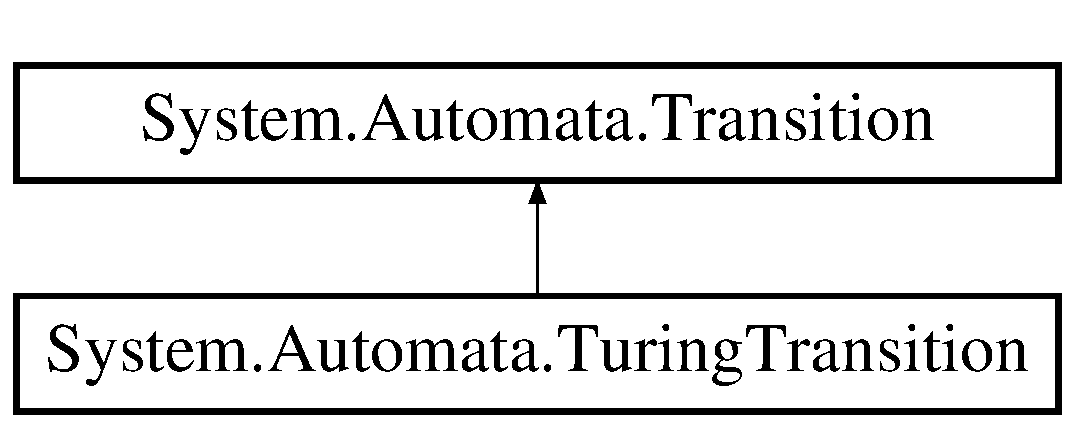
\includegraphics[height=2.000000cm]{class_system_1_1_automata_1_1_turing_transition}
\end{center}
\end{figure}
\subsection*{Public Member Functions}
\begin{DoxyCompactItemize}
\item 
\mbox{\hyperlink{class_system_1_1_automata_1_1_turing_transition_a67564840226244a1f36666913d299469}{Turing\+Transition}} (\mbox{\hyperlink{class_system_1_1_automata_1_1_state}{State}} p, char x, \mbox{\hyperlink{class_system_1_1_automata_1_1_state}{State}} q, char y, \mbox{\hyperlink{class_system_1_1_automata_1_1_turing_machine_aa253c3820befa3cfdd3d17b2d8fdd2d9}{Turing\+Machine.\+Direction}} d)
\item 
\mbox{\Hypertarget{class_system_1_1_automata_1_1_turing_transition_af59b7537f01077c715bc69eaa6b28544}\label{class_system_1_1_automata_1_1_turing_transition_af59b7537f01077c715bc69eaa6b28544}} 
override string {\bfseries To\+String} ()
\end{DoxyCompactItemize}
\subsection*{Properties}
\begin{DoxyCompactItemize}
\item 
char \mbox{\hyperlink{class_system_1_1_automata_1_1_turing_transition_a1837a0ade7ba5eae701f731ec5fb6dc7}{B}}\hspace{0.3cm}{\ttfamily  \mbox{[}get\mbox{]}}
\begin{DoxyCompactList}\small\item\em The character to replace the current tape cell with. \end{DoxyCompactList}\item 
\mbox{\hyperlink{class_system_1_1_automata_1_1_turing_machine_aa253c3820befa3cfdd3d17b2d8fdd2d9}{Turing\+Machine.\+Direction}} \mbox{\hyperlink{class_system_1_1_automata_1_1_turing_transition_af02531641bd2e8805ad322c253a34660}{Direction}}\hspace{0.3cm}{\ttfamily  \mbox{[}get\mbox{]}}
\begin{DoxyCompactList}\small\item\em The direction to move the tape head in. \end{DoxyCompactList}\end{DoxyCompactItemize}


\subsection{Detailed Description}
A transition for a Turing machine 



\subsection{Constructor \& Destructor Documentation}
\mbox{\Hypertarget{class_system_1_1_automata_1_1_turing_transition_a67564840226244a1f36666913d299469}\label{class_system_1_1_automata_1_1_turing_transition_a67564840226244a1f36666913d299469}} 
\index{System\+::\+Automata\+::\+Turing\+Transition@{System\+::\+Automata\+::\+Turing\+Transition}!Turing\+Transition@{Turing\+Transition}}
\index{Turing\+Transition@{Turing\+Transition}!System\+::\+Automata\+::\+Turing\+Transition@{System\+::\+Automata\+::\+Turing\+Transition}}
\subsubsection{\texorpdfstring{Turing\+Transition()}{TuringTransition()}}
{\footnotesize\ttfamily System.\+Automata.\+Turing\+Transition.\+Turing\+Transition (\begin{DoxyParamCaption}\item[{\mbox{\hyperlink{class_system_1_1_automata_1_1_state}{State}}}]{p,  }\item[{char}]{x,  }\item[{\mbox{\hyperlink{class_system_1_1_automata_1_1_state}{State}}}]{q,  }\item[{char}]{y,  }\item[{\mbox{\hyperlink{class_system_1_1_automata_1_1_turing_machine_aa253c3820befa3cfdd3d17b2d8fdd2d9}{Turing\+Machine.\+Direction}}}]{d }\end{DoxyParamCaption})}


\begin{DoxyParams}{Parameters}
{\em p} & The current state.\\
\hline
{\em x} & The current tape cell contents.\\
\hline
{\em q} & The next state.\\
\hline
{\em y} & The character to replace the tape cell with.\\
\hline
{\em d} & The direction to move the tape head after transitioning.\\
\hline
\end{DoxyParams}


\subsection{Property Documentation}
\mbox{\Hypertarget{class_system_1_1_automata_1_1_turing_transition_a1837a0ade7ba5eae701f731ec5fb6dc7}\label{class_system_1_1_automata_1_1_turing_transition_a1837a0ade7ba5eae701f731ec5fb6dc7}} 
\index{System\+::\+Automata\+::\+Turing\+Transition@{System\+::\+Automata\+::\+Turing\+Transition}!B@{B}}
\index{B@{B}!System\+::\+Automata\+::\+Turing\+Transition@{System\+::\+Automata\+::\+Turing\+Transition}}
\subsubsection{\texorpdfstring{B}{B}}
{\footnotesize\ttfamily char System.\+Automata.\+Turing\+Transition.\+B\hspace{0.3cm}{\ttfamily [get]}}



The character to replace the current tape cell with. 

\mbox{\Hypertarget{class_system_1_1_automata_1_1_turing_transition_af02531641bd2e8805ad322c253a34660}\label{class_system_1_1_automata_1_1_turing_transition_af02531641bd2e8805ad322c253a34660}} 
\index{System\+::\+Automata\+::\+Turing\+Transition@{System\+::\+Automata\+::\+Turing\+Transition}!Direction@{Direction}}
\index{Direction@{Direction}!System\+::\+Automata\+::\+Turing\+Transition@{System\+::\+Automata\+::\+Turing\+Transition}}
\subsubsection{\texorpdfstring{Direction}{Direction}}
{\footnotesize\ttfamily \mbox{\hyperlink{class_system_1_1_automata_1_1_turing_machine_aa253c3820befa3cfdd3d17b2d8fdd2d9}{Turing\+Machine.\+Direction}} System.\+Automata.\+Turing\+Transition.\+Direction\hspace{0.3cm}{\ttfamily [get]}}



The direction to move the tape head in. 



The documentation for this class was generated from the following file\+:\begin{DoxyCompactItemize}
\item 
System.\+Automata/Turing\+Transition.\+cs\end{DoxyCompactItemize}

\hypertarget{class_system_1_1_automata_1_1_turing_transition_function}{}\section{System.\+Automata.\+Turing\+Transition\+Function Class Reference}
\label{class_system_1_1_automata_1_1_turing_transition_function}\index{System.\+Automata.\+Turing\+Transition\+Function@{System.\+Automata.\+Turing\+Transition\+Function}}


A collection of state transition mappings for P\+D\+As  


Inheritance diagram for System.\+Automata.\+Turing\+Transition\+Function\+:\begin{figure}[H]
\begin{center}
\leavevmode
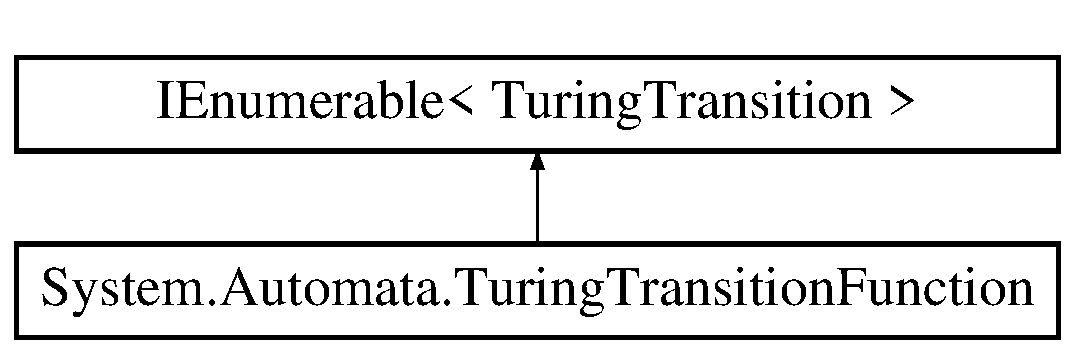
\includegraphics[height=2.000000cm]{class_system_1_1_automata_1_1_turing_transition_function}
\end{center}
\end{figure}
\subsection*{Public Member Functions}
\begin{DoxyCompactItemize}
\item 
\mbox{\Hypertarget{class_system_1_1_automata_1_1_turing_transition_function_aaa2341e389d0d2a4291b5379bc8e110f}\label{class_system_1_1_automata_1_1_turing_transition_function_aaa2341e389d0d2a4291b5379bc8e110f}} 
{\bfseries Turing\+Transition\+Function} (params \mbox{\hyperlink{class_system_1_1_automata_1_1_turing_transition}{Turing\+Transition}}\mbox{[}$\,$\mbox{]} t)
\item 
\mbox{\Hypertarget{class_system_1_1_automata_1_1_turing_transition_function_a3b2a9439a7742e55d003002065746e7e}\label{class_system_1_1_automata_1_1_turing_transition_function_a3b2a9439a7742e55d003002065746e7e}} 
void {\bfseries Add} (\mbox{\hyperlink{class_system_1_1_automata_1_1_turing_transition}{Turing\+Transition}} t)
\item 
\mbox{\Hypertarget{class_system_1_1_automata_1_1_turing_transition_function_a7db6f1271627564f81e7354709248af6}\label{class_system_1_1_automata_1_1_turing_transition_function_a7db6f1271627564f81e7354709248af6}} 
bool {\bfseries Contains} (\mbox{\hyperlink{class_system_1_1_automata_1_1_turing_transition}{Turing\+Transition}} t)
\item 
\mbox{\Hypertarget{class_system_1_1_automata_1_1_turing_transition_function_aa297d69ac197b1887ef5769a27b1a2b9}\label{class_system_1_1_automata_1_1_turing_transition_function_aa297d69ac197b1887ef5769a27b1a2b9}} 
bool {\bfseries Exists} (Predicate$<$ \mbox{\hyperlink{class_system_1_1_automata_1_1_turing_transition}{Turing\+Transition}} $>$ p)
\item 
\mbox{\Hypertarget{class_system_1_1_automata_1_1_turing_transition_function_a7be9f8007ad5e06b2b09e73c15e4bd81}\label{class_system_1_1_automata_1_1_turing_transition_function_a7be9f8007ad5e06b2b09e73c15e4bd81}} 
I\+Enumerator$<$ \mbox{\hyperlink{class_system_1_1_automata_1_1_turing_transition}{Turing\+Transition}} $>$ {\bfseries Get\+Enumerator} ()
\end{DoxyCompactItemize}
\subsection*{Public Attributes}
\begin{DoxyCompactItemize}
\item 
\mbox{\Hypertarget{class_system_1_1_automata_1_1_turing_transition_function_a768db7b6eb2d61eeb49ea912da85ba8f}\label{class_system_1_1_automata_1_1_turing_transition_function_a768db7b6eb2d61eeb49ea912da85ba8f}} 
int {\bfseries Count} =$>$ \+\_\+trans.\+Count
\item 
\mbox{\hyperlink{class_system_1_1_automata_1_1_turing_transition}{Turing\+Transition}} \mbox{[}$\,$\mbox{]} {\bfseries this\mbox{[}\+State p, char a\mbox{]}}
\end{DoxyCompactItemize}


\subsection{Detailed Description}
A collection of state transition mappings for P\+D\+As 



\subsection{Member Data Documentation}
\mbox{\Hypertarget{class_system_1_1_automata_1_1_turing_transition_function_a1f3d2faa8ea2a3b623c2e7cb55c56290}\label{class_system_1_1_automata_1_1_turing_transition_function_a1f3d2faa8ea2a3b623c2e7cb55c56290}} 
\index{System\+::\+Automata\+::\+Turing\+Transition\+Function@{System\+::\+Automata\+::\+Turing\+Transition\+Function}!this\mbox{[}\+State p, char a\mbox{]}@{this[State p, char a]}}
\index{this\mbox{[}\+State p, char a\mbox{]}@{this[State p, char a]}!System\+::\+Automata\+::\+Turing\+Transition\+Function@{System\+::\+Automata\+::\+Turing\+Transition\+Function}}
\subsubsection{\texorpdfstring{this[State p, char a]}{this[State p, char a]}}
{\footnotesize\ttfamily \mbox{\hyperlink{class_system_1_1_automata_1_1_turing_transition}{Turing\+Transition}} \mbox{[}$\,$\mbox{]} System.\+Automata.\+Turing\+Transition\+Function.\+this\mbox{[}\mbox{\hyperlink{class_system_1_1_automata_1_1_state}{State}} p, char a\mbox{]}}

{\bfseries Initial value\+:}
\begin{DoxyCode}
=>
            \_trans.Where(x => x.P.Equals(p) && x.A == a).ToArray()
\end{DoxyCode}


The documentation for this class was generated from the following file\+:\begin{DoxyCompactItemize}
\item 
System.\+Automata/Turing\+Transition\+Function.\+cs\end{DoxyCompactItemize}

%--- End generated contents ---

% Index
\backmatter
\newpage
\phantomsection
\clearemptydoublepage
\addcontentsline{toc}{chapter}{Index}
\printindex

\end{document}
